%*******************************************************************************
%****************************** Appendix E *************************************
%*******************************************************************************
\chapter{Additional results for HHI experiment} \label{appendix:e}

% **************************** Define Graphics Path **************************
\graphicspath{{figs/appendixE/PDF/}}


\section{Time Series} \label{appendix:e:ts}

Time series for twenty participants with a window length size of 500 samples
of horizontal arm movements (Figs. \ref{fig:aH-sg0}, \ref{fig:aH-sg1}, \ref{fig:aH-sg2})
and vertical arm movements (Figs. \ref{fig:aV-sg0}, \ref{fig:aV-sg1}, \ref{fig:aV-sg2}).
For the remained window size lengths of time series data, we refer
the reader to download the data and code at \cite{xochicale2018}.
%%---------------------------------(FIGURE)-------------------------------------
\begin{figure}
\centering
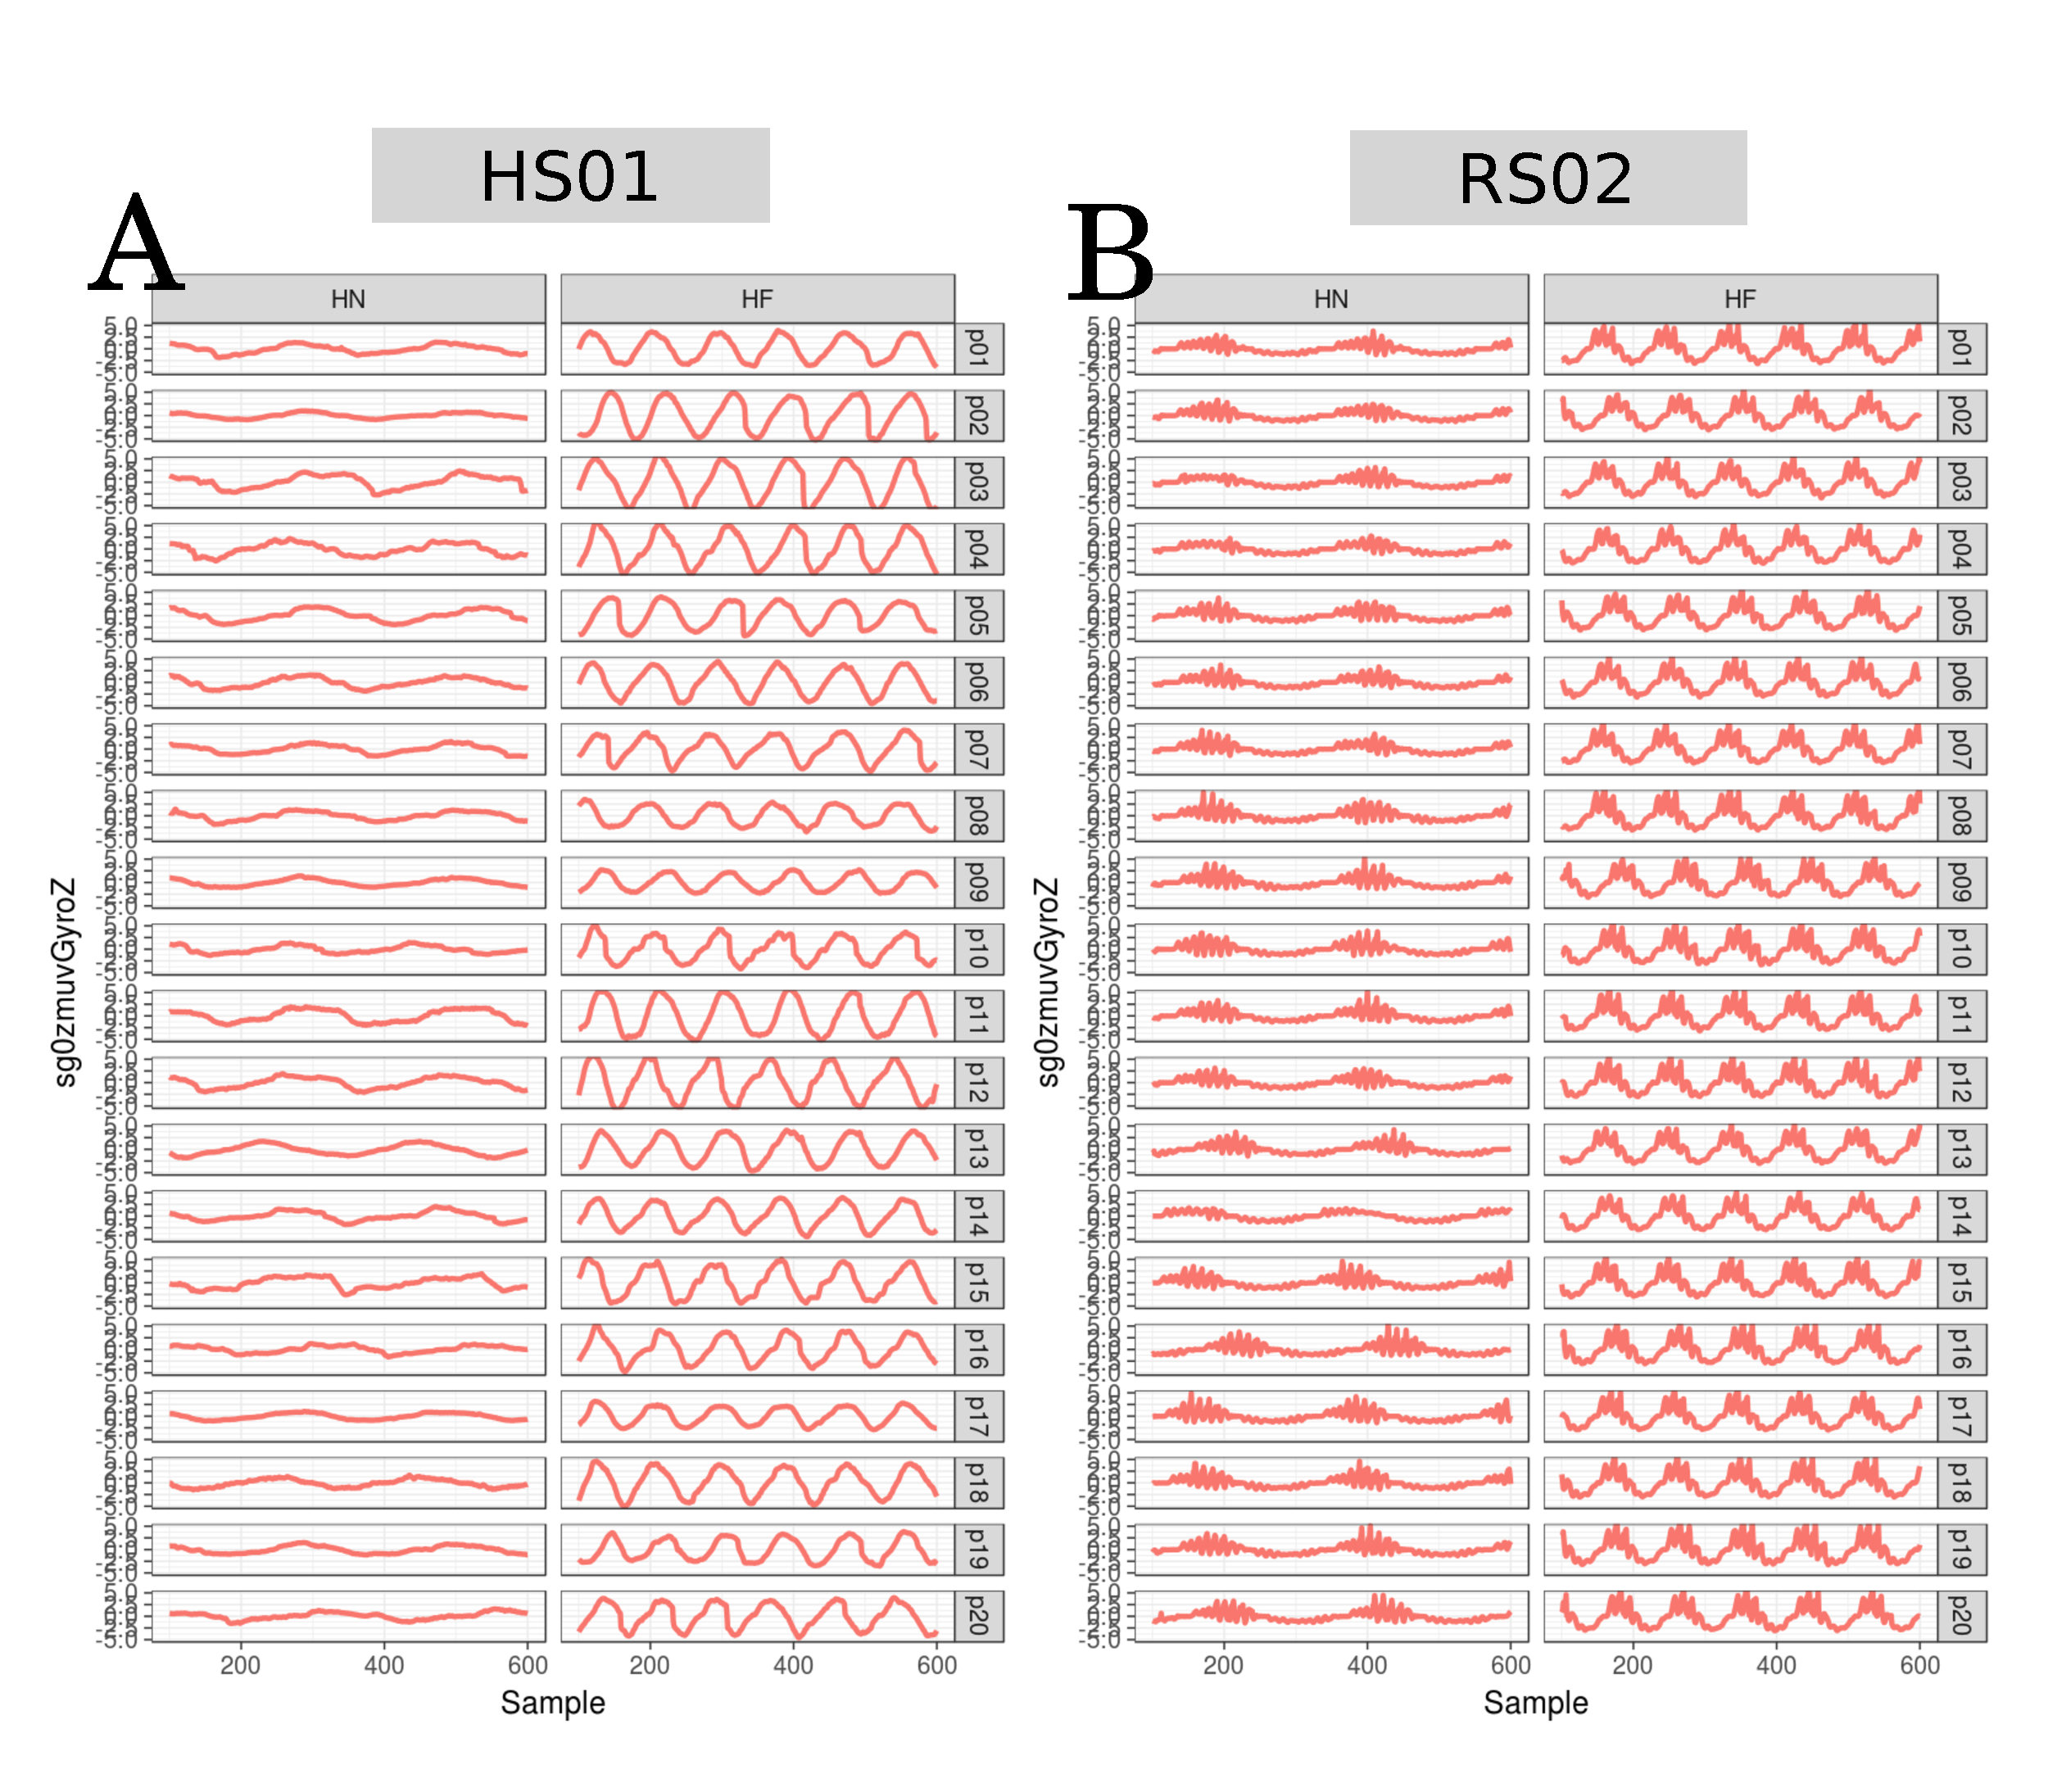
\includegraphics[width=1.0\textwidth]{aH-sg0}
    	\caption
	[Time series for horizontal arm movements (sg0) ]{
	{\bf Time series for horizontal arm movements (sg0)}
		Time series for sg0zmuvGyroZ for twenty participants 
		($p01$ to  $p20$) 
		for horizontal movements in normal (HN) and horizontal faster (HF) 
		velocity with sensors attached to the participant wrist (HS01)
		and to the humanoid wrist (RS02).
	R code to reproduce the figure is available from \cite{xochicale2018}.
        }
    \label{fig:aH-sg0}
\end{figure}
%%---------------------------------(FIGURE)-----------------------------------

%%---------------------------------(FIGURE)-------------------------------------
\begin{figure}
\centering
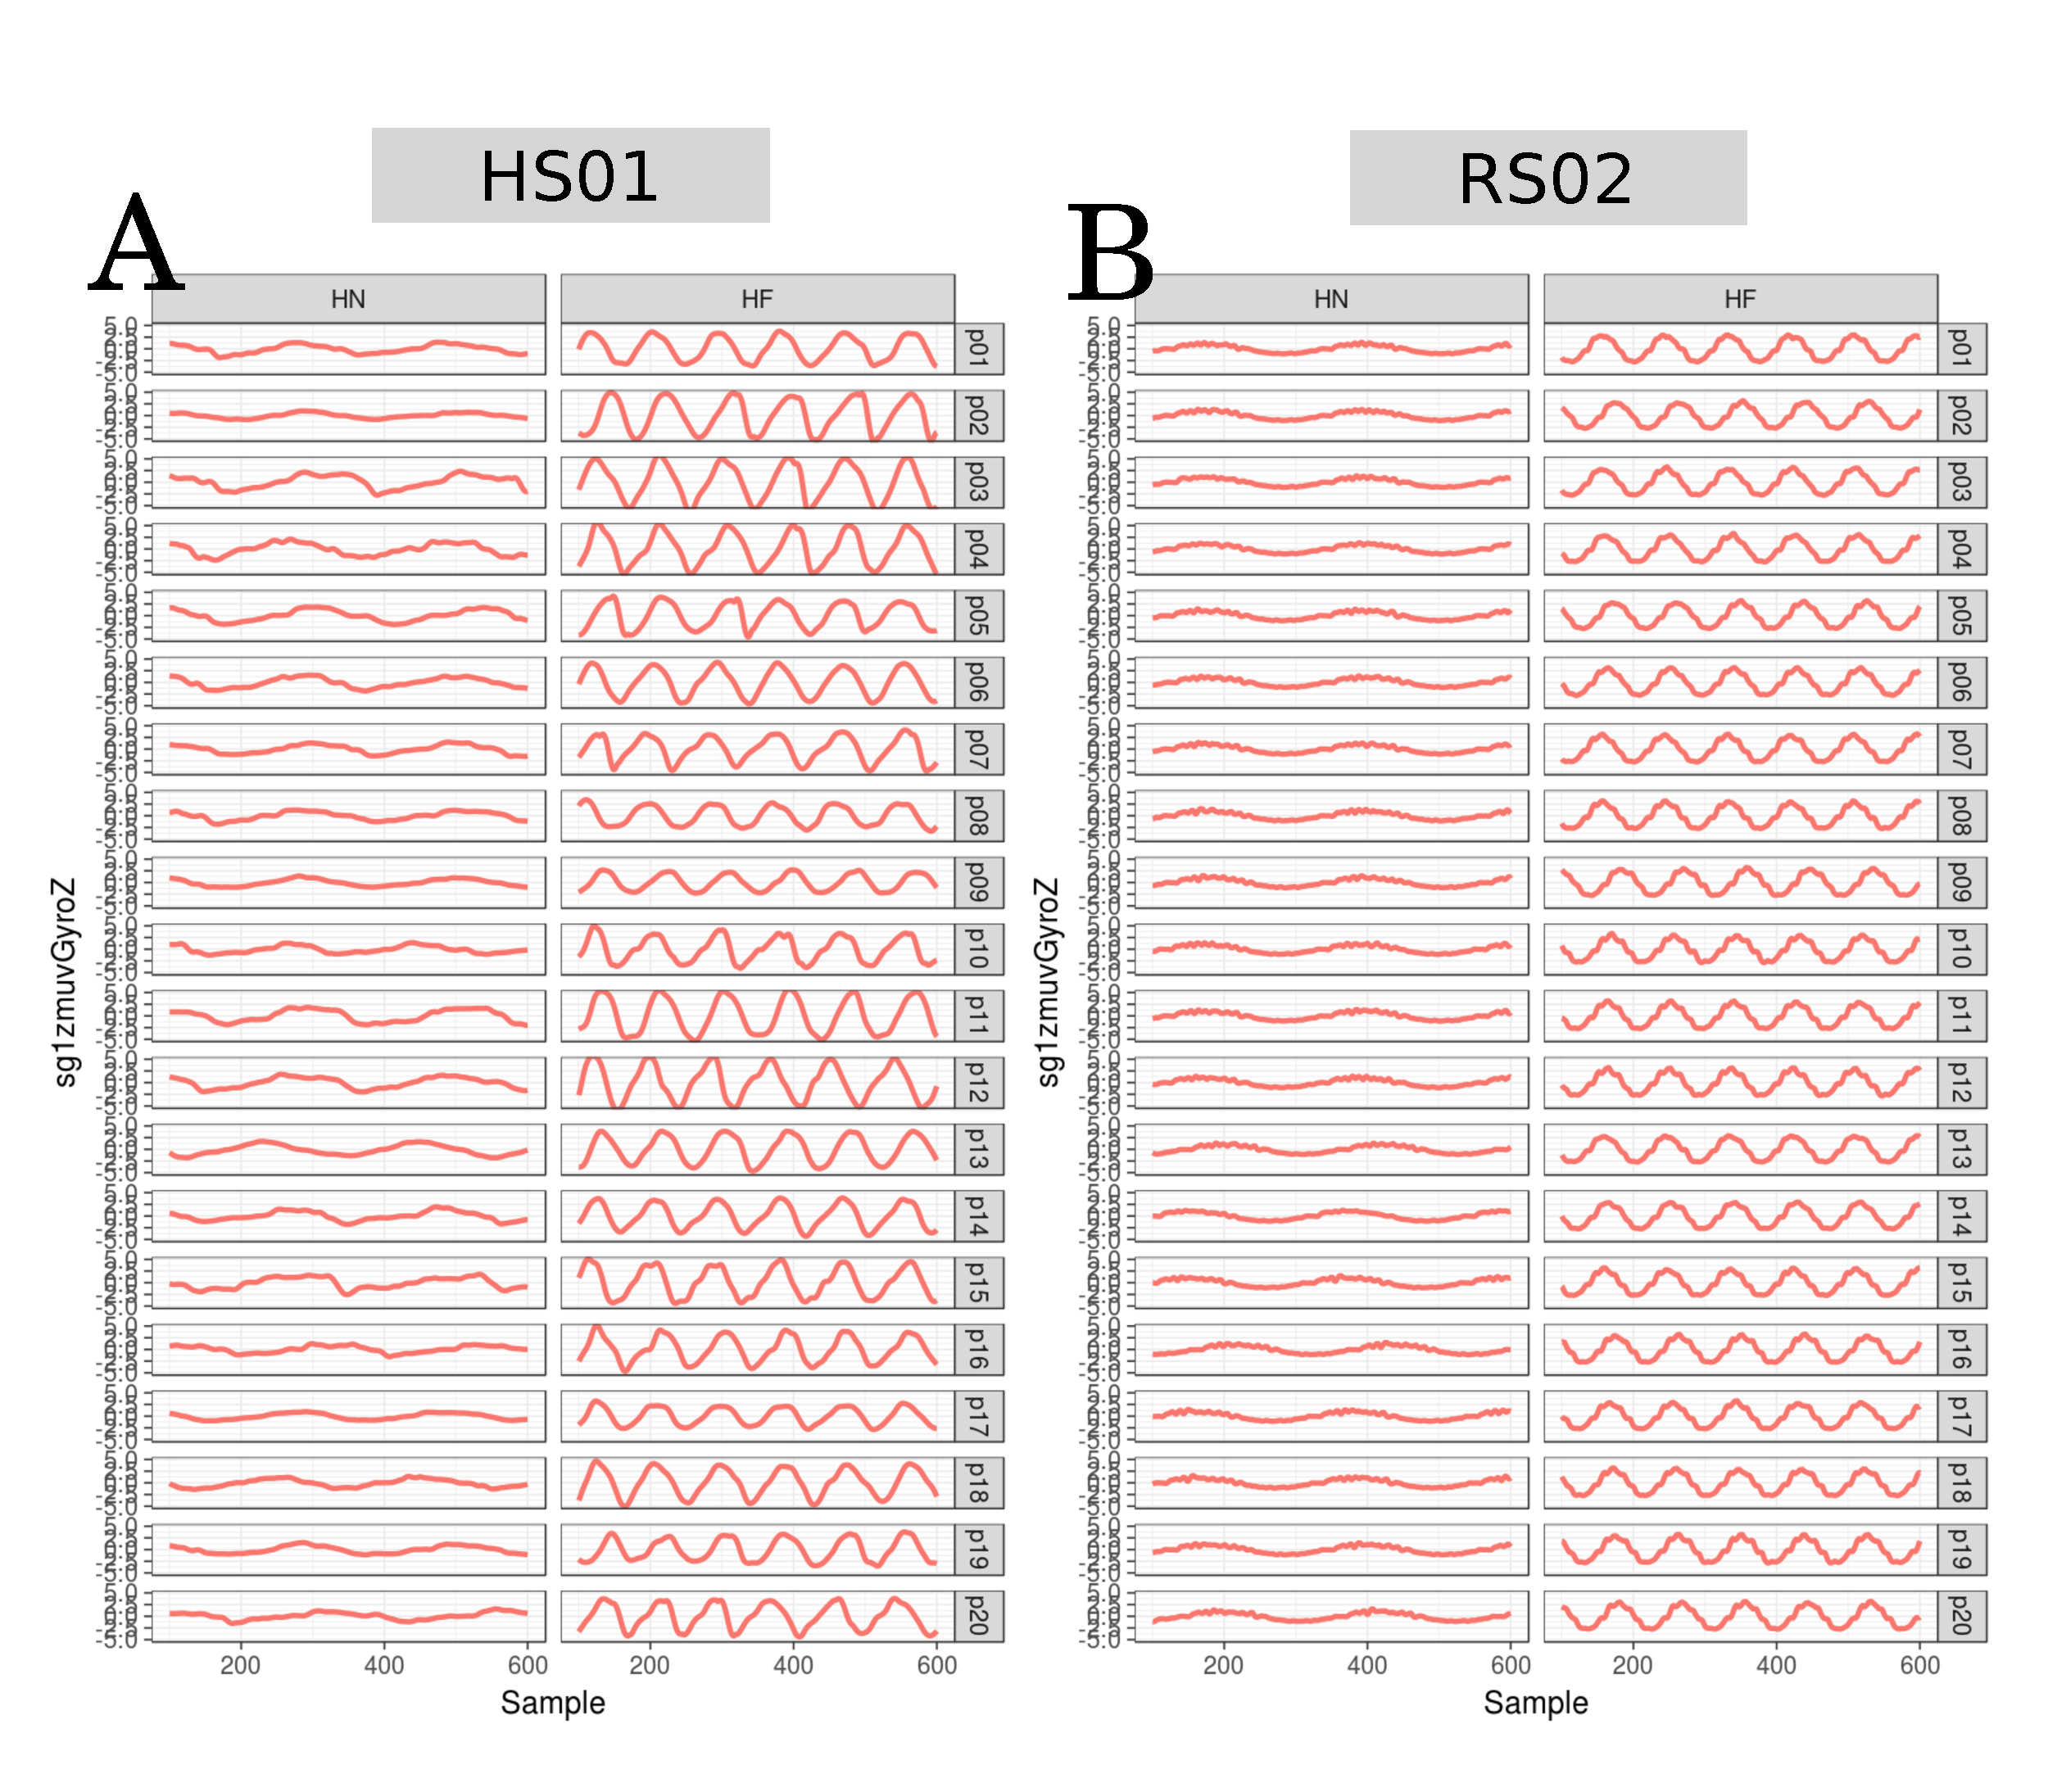
\includegraphics[width=1.0\textwidth]{aH-sg1}
    	\caption
	[Time series for horizontal arm movements (sg1) ]{
	{\bf Time series for horizontal arm movements (sg1)}
		Time series for sg0zmuvGyroZ for twenty participants 
		($p01$ to  $p20$) 
		for horizontal movements in normal (HN) and horizontal faster (HF) 
		velocity with sensors attached to the participant wrist (HS01)
		and to the humanoid wrist (RS02).
	R code to reproduce the figure is available from \cite{xochicale2018}.
        }
    \label{fig:aH-sg1}
\end{figure}
%%---------------------------------(FIGURE)-----------------------------------

%%---------------------------------(FIGURE)-------------------------------------
\begin{figure}
\centering
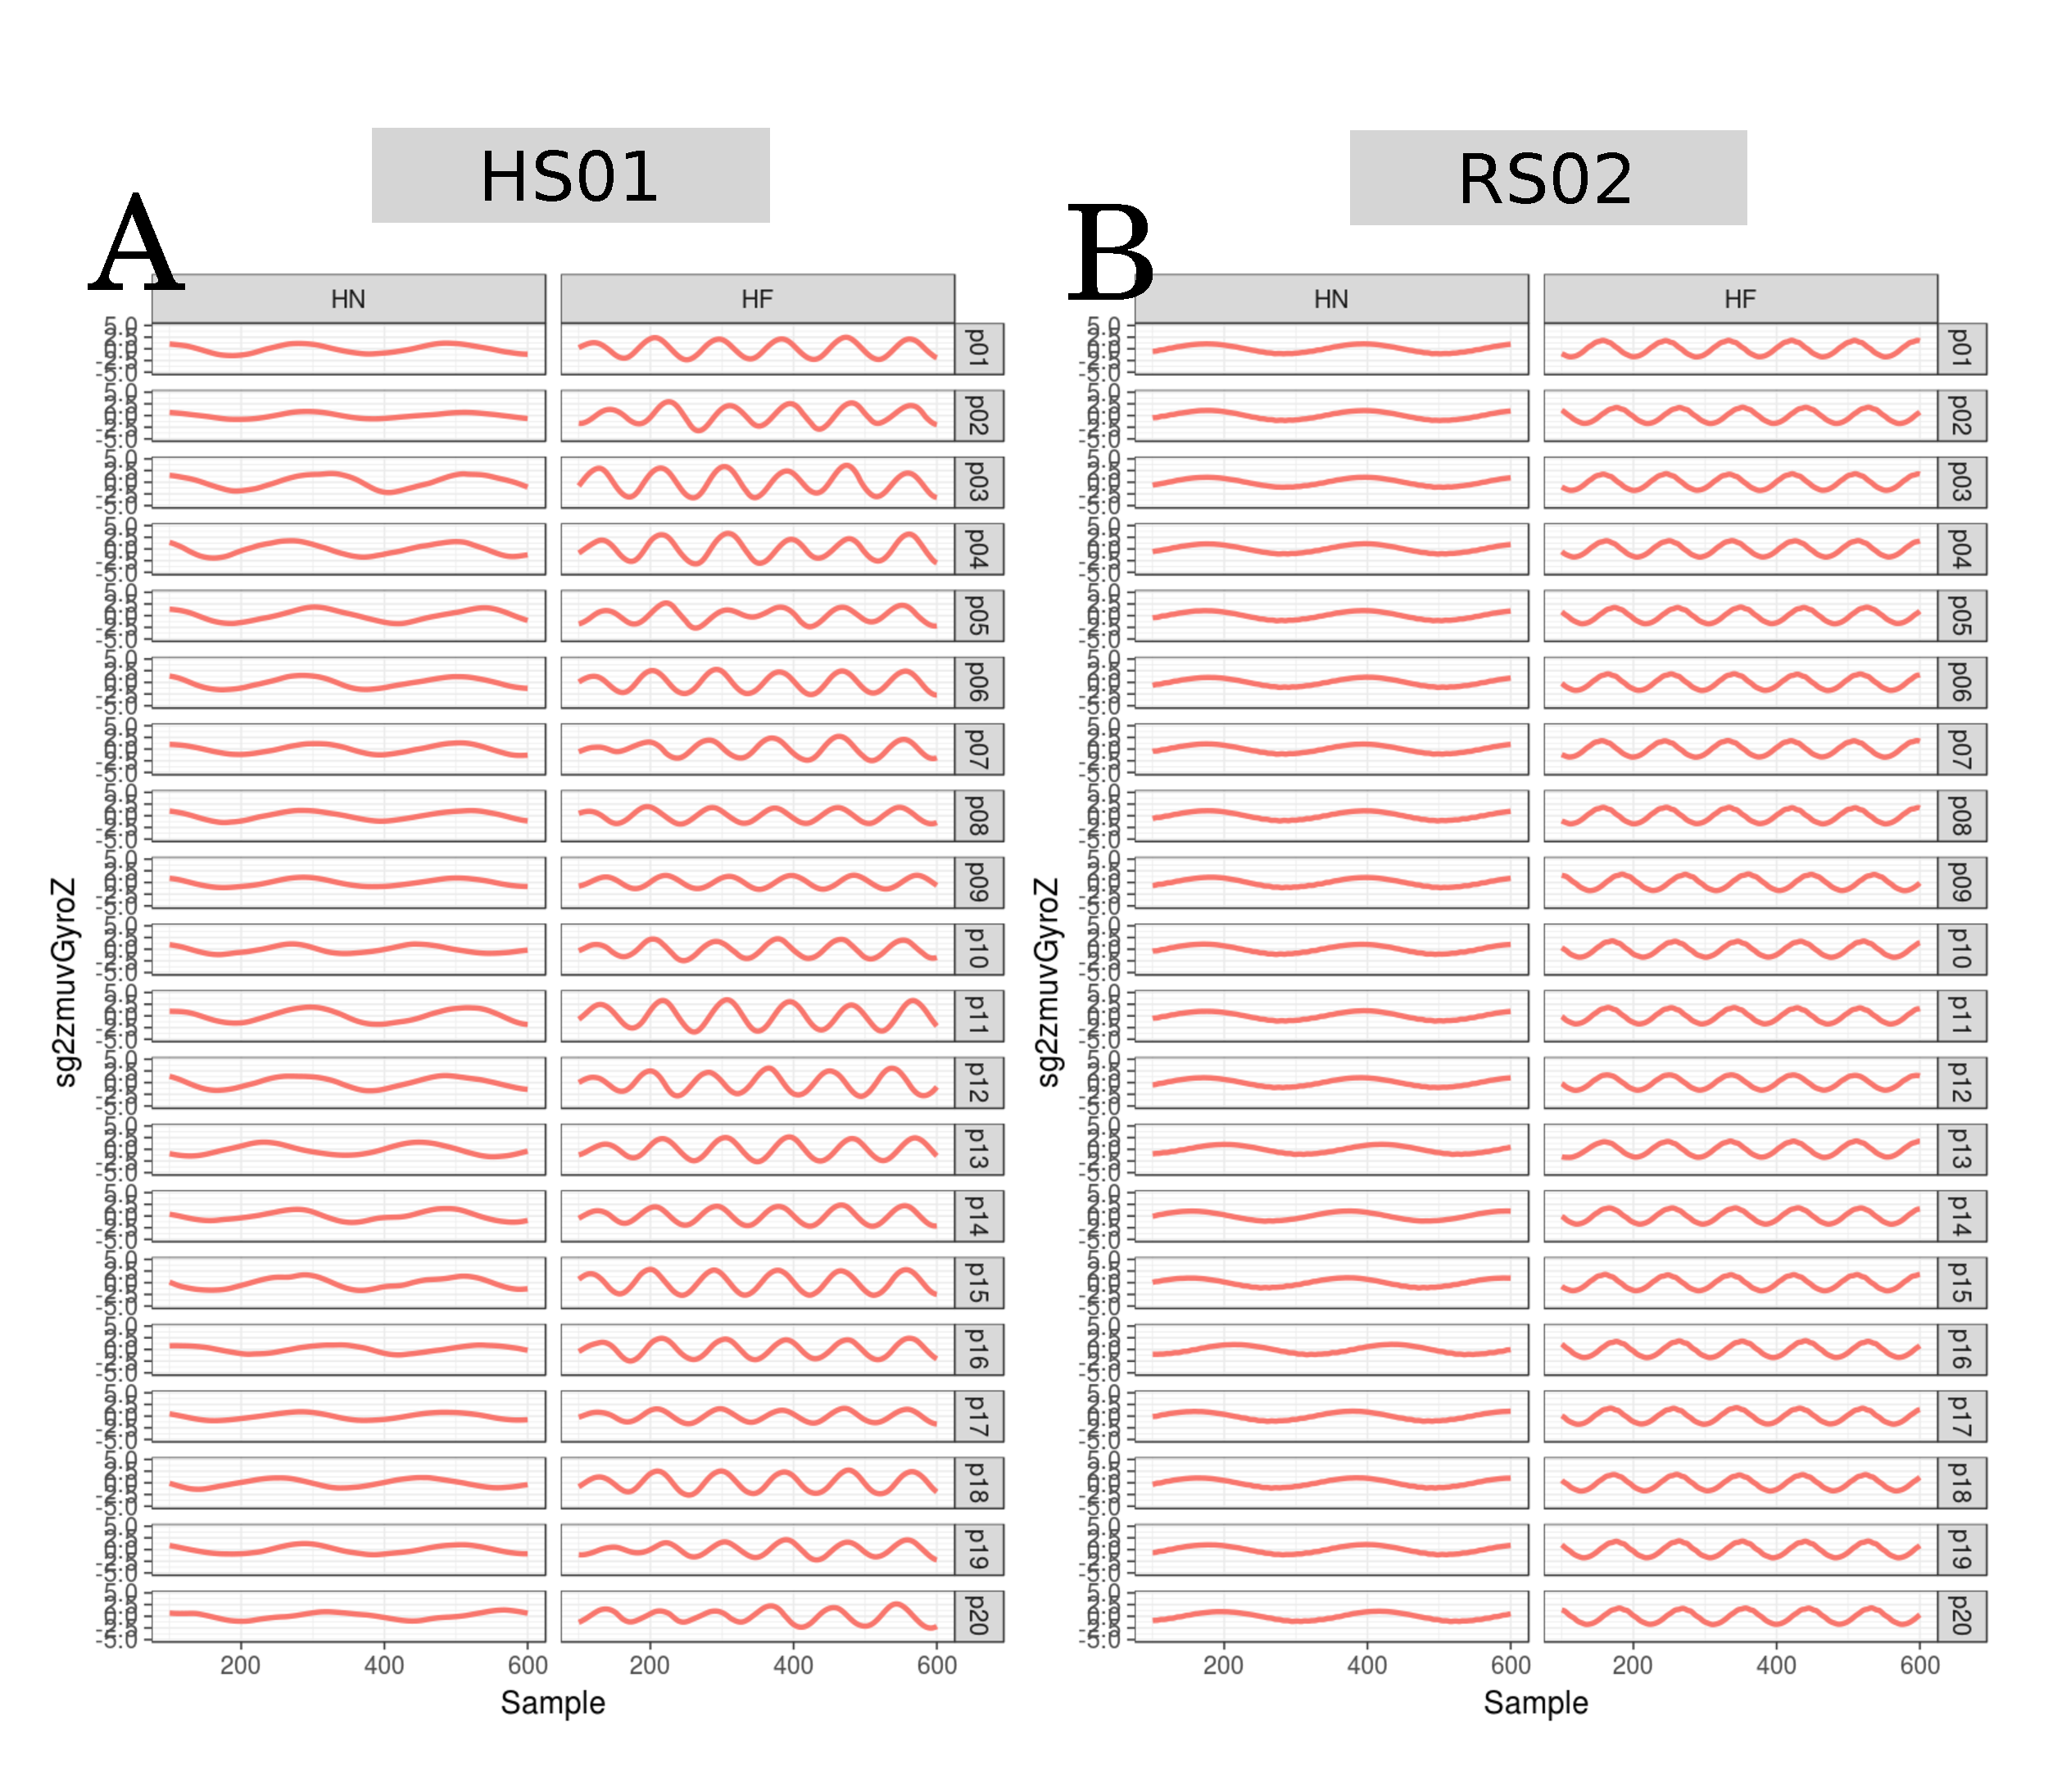
\includegraphics[width=1.0\textwidth]{aH-sg2}
    	\caption
	[Time series for horizontal arm movements (sg2) ]{
	{\bf Time series for horizontal arm movements (sg2)}
		Time series for sg0zmuvGyroZ for twenty participants 
		($p01$ to  $p20$) 
		for horizontal movements in normal (HN) and horizontal faster (HF) 
		velocity with sensors attached to the participant wrist (HS01)
		and to the humanoid wrist (RS02).
	R code to reproduce the figure is available from \cite{xochicale2018}.
        }
    \label{fig:aH-sg2}
\end{figure}
%%---------------------------------(FIGURE)-----------------------------------





%%---------------------------------(FIGURE)-------------------------------------
\begin{figure}
\centering
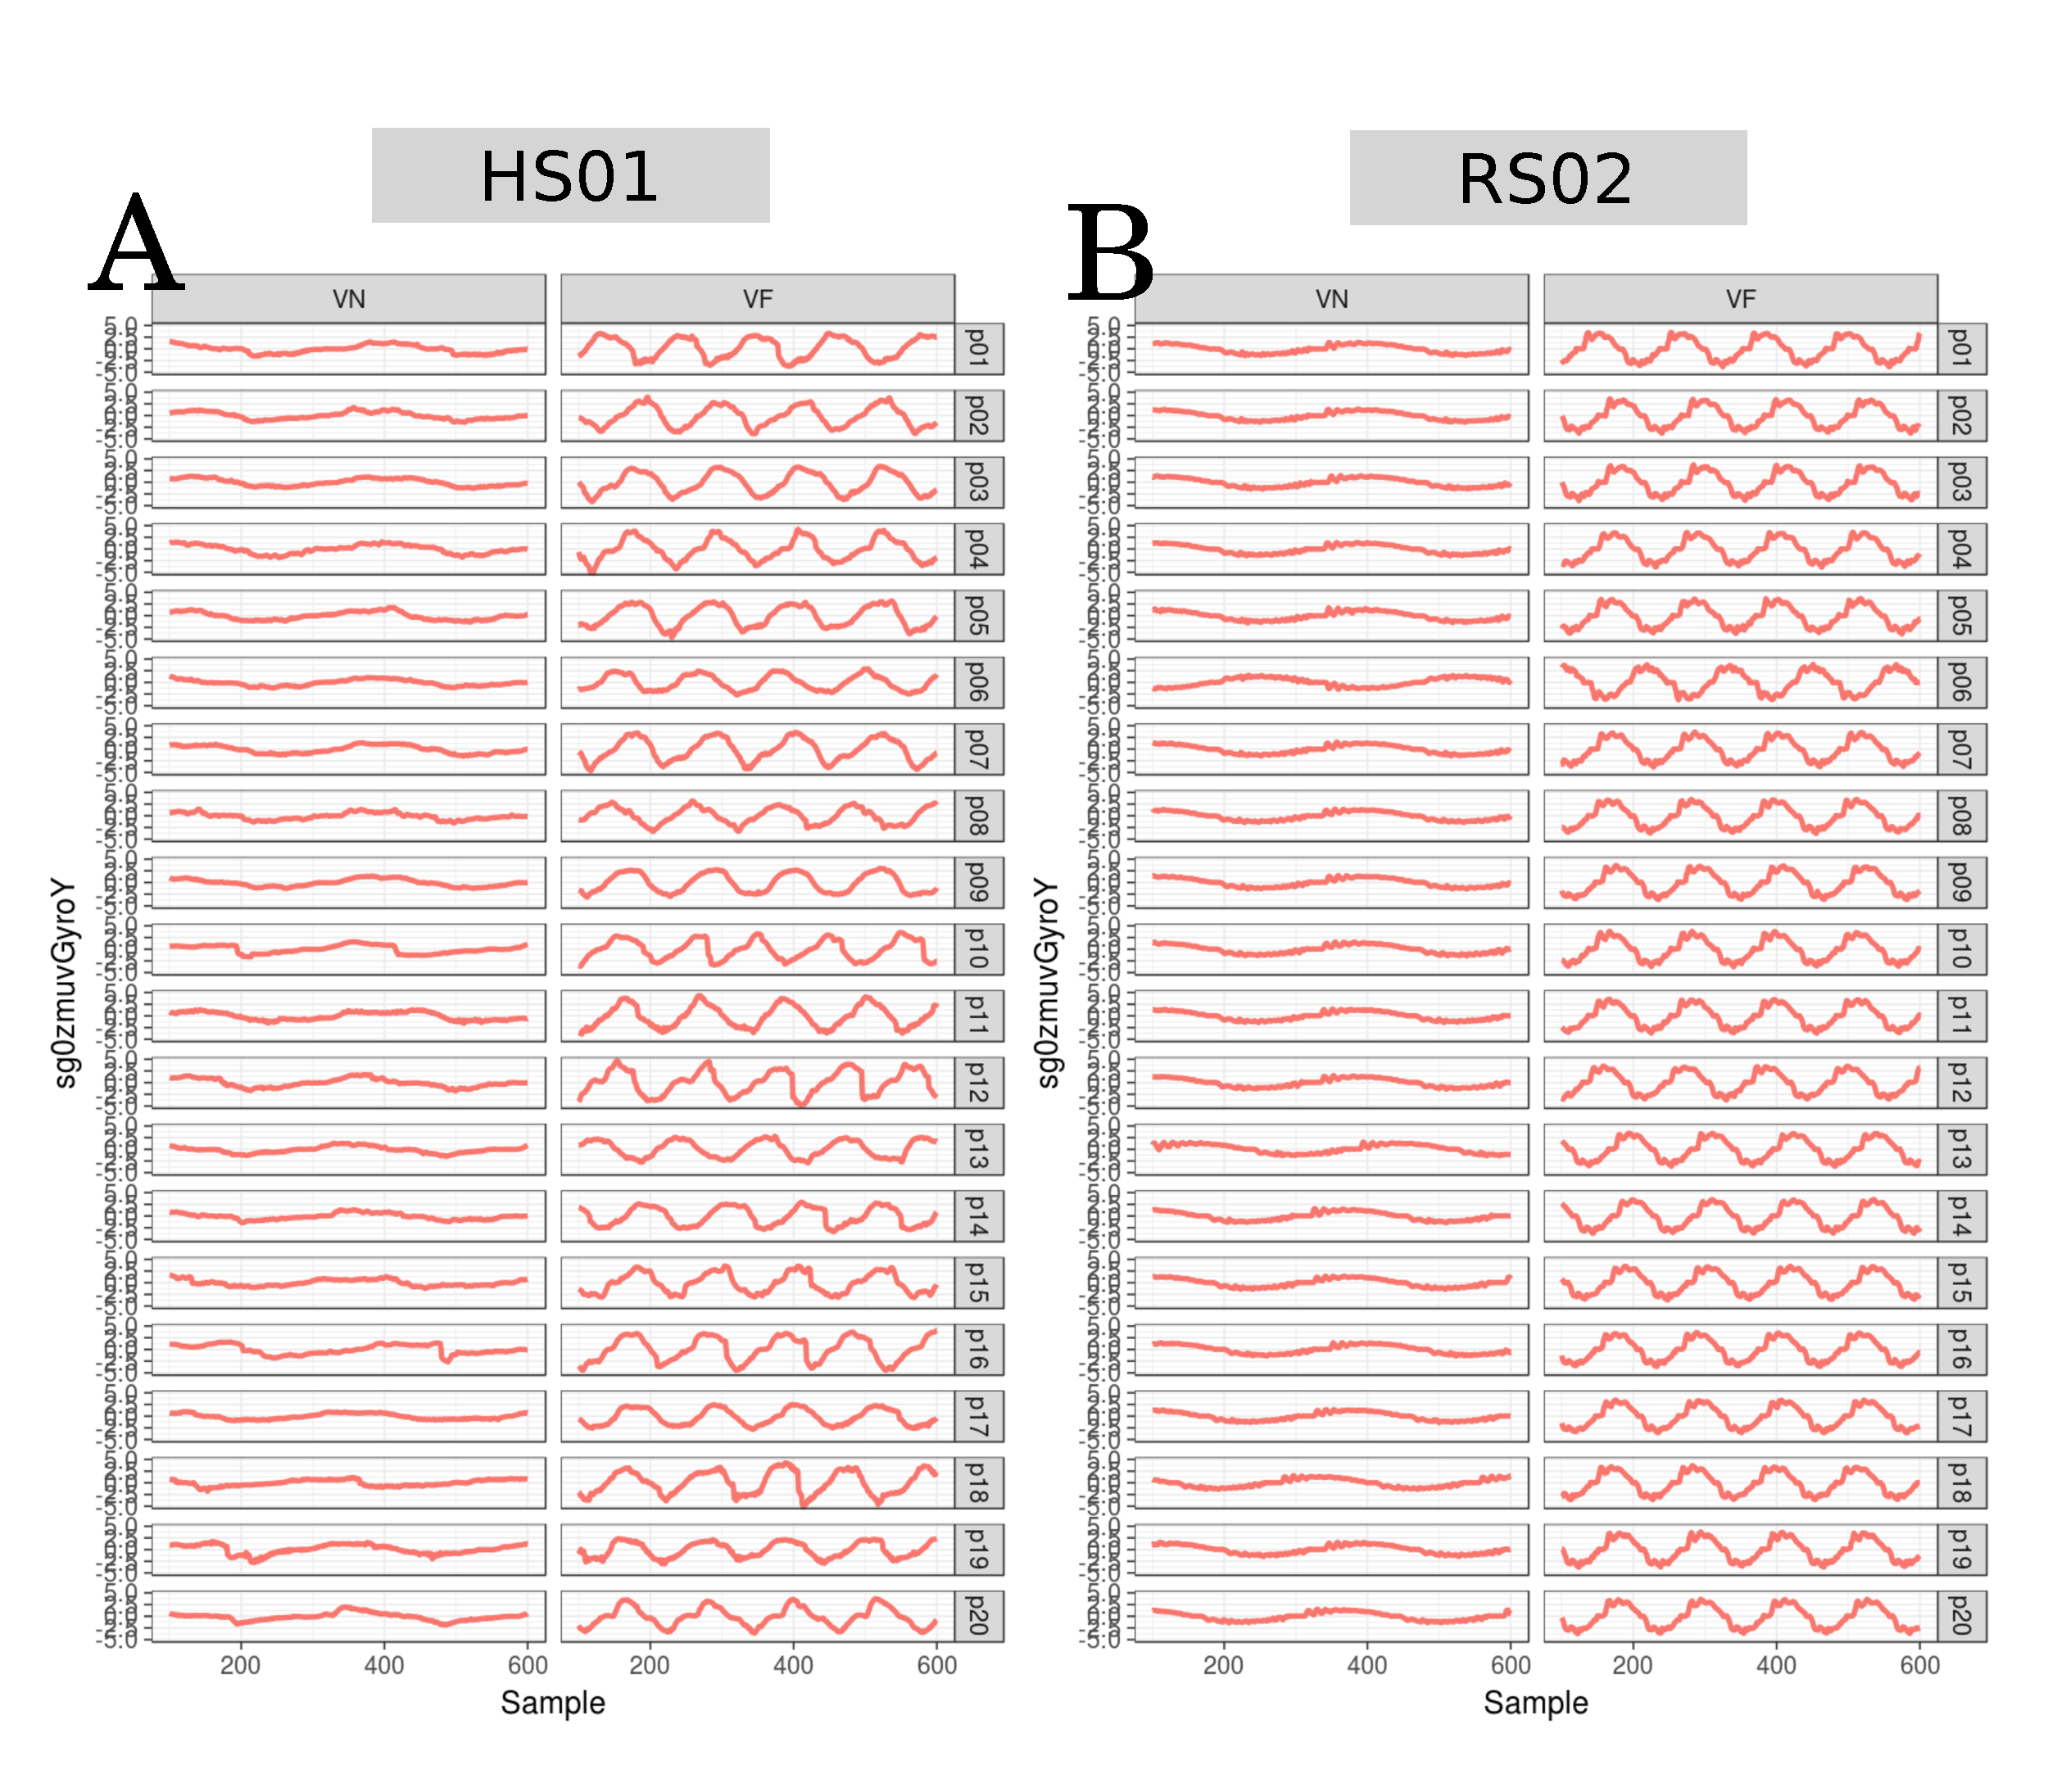
\includegraphics[width=1.0\textwidth]{aV-sg0}
    	\caption
	[Time series for vertical arm movements (sg0) ]{
	{\bf Time series for vertical arm movements (sg0)}
		Time series for sg0zmuvGyroY for twenty participants 
		($p01$ to  $p20$) 
		for vertical movements in normal (HN) and horizontal faster (HF) 
		velocity with sensors attached to the participant wrist (HS01)
		and to the humanoid wrist (RS02).
	R code to reproduce the figure is available from \cite{xochicale2018}.
        }
    \label{fig:aV-sg0}
\end{figure}
%%---------------------------------(FIGURE)-----------------------------------

%%---------------------------------(FIGURE)-------------------------------------
\begin{figure}
\centering
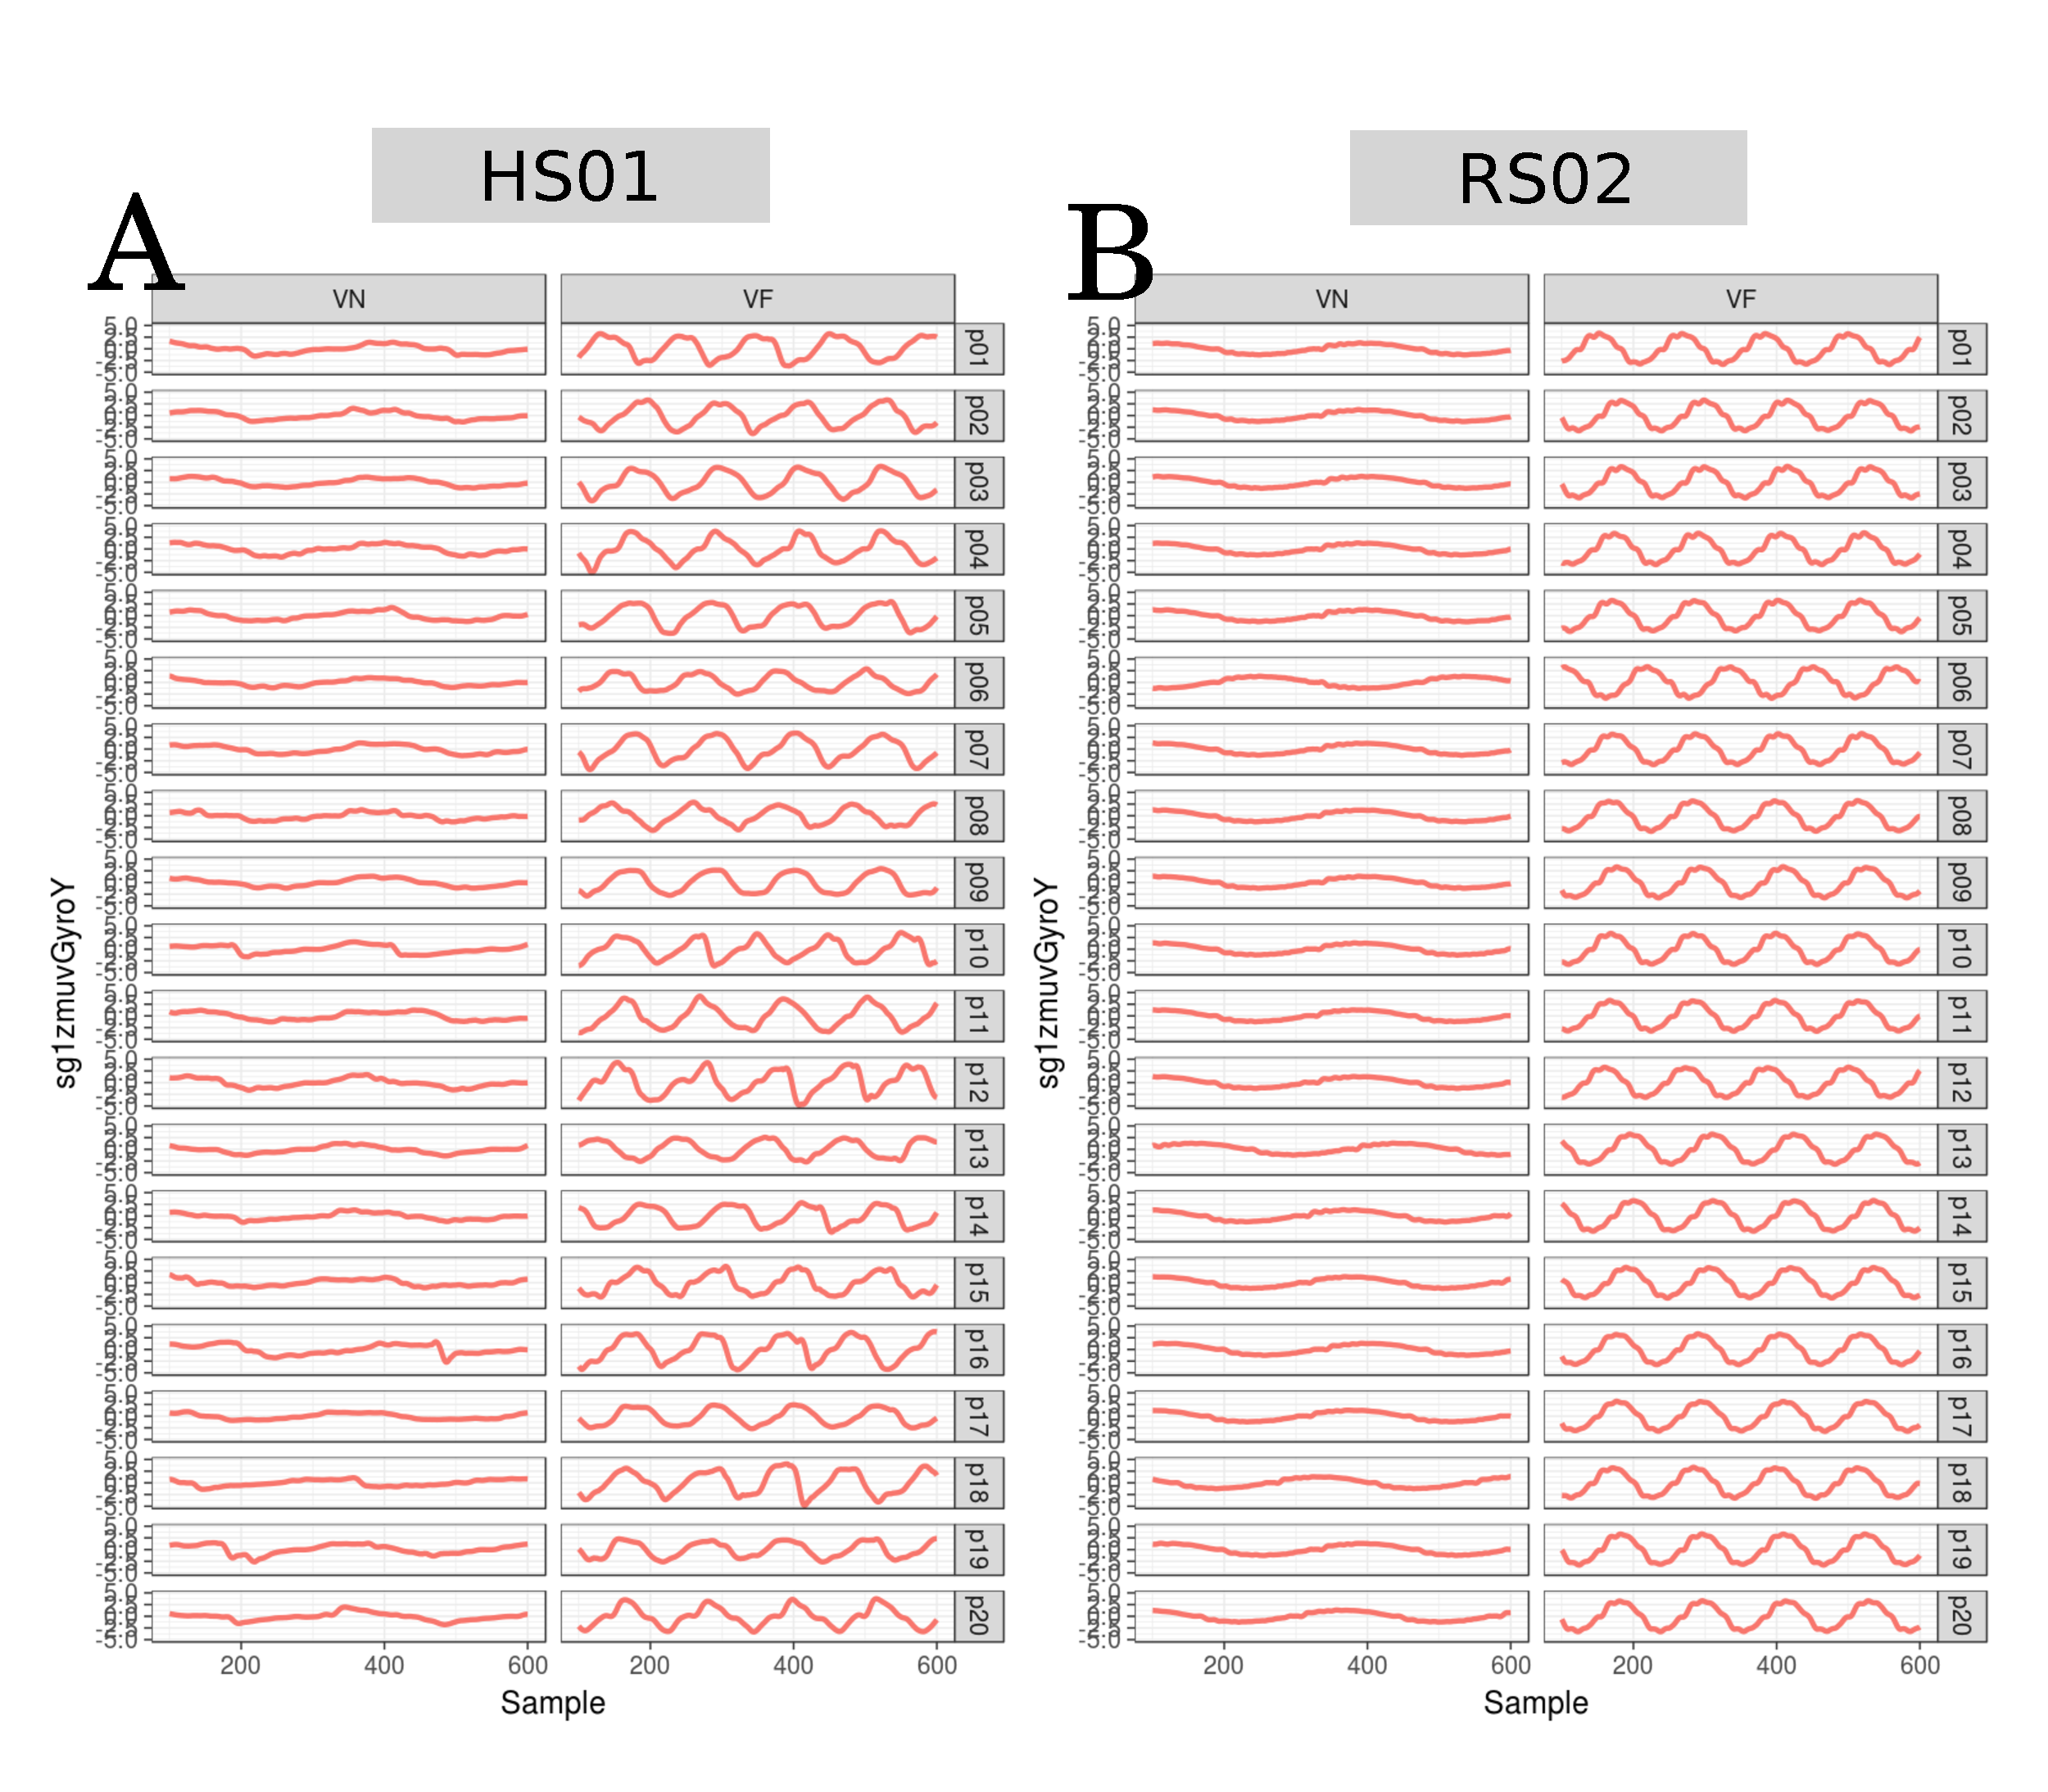
\includegraphics[width=1.0\textwidth]{aV-sg1}
    	\caption
	[Time series for vertical arm movements (sg1) ]{
	{\bf Time series for vertical arm movements (sg1)}
		Time series for sg0zmuvGyroY for twenty participants 
		($p01$ to  $p20$) 
		for horizontal movements in normal (HN) and horizontal faster (HF) 
		velocity with sensors attached to the participant wrist (HS01)
		and to the humanoid wrist (RS02).
	R code to reproduce the figure is available from \cite{xochicale2018}.
        }
    \label{fig:aV-sg1}
\end{figure}
%%---------------------------------(FIGURE)-----------------------------------

%%---------------------------------(FIGURE)-------------------------------------
\begin{figure}
\centering
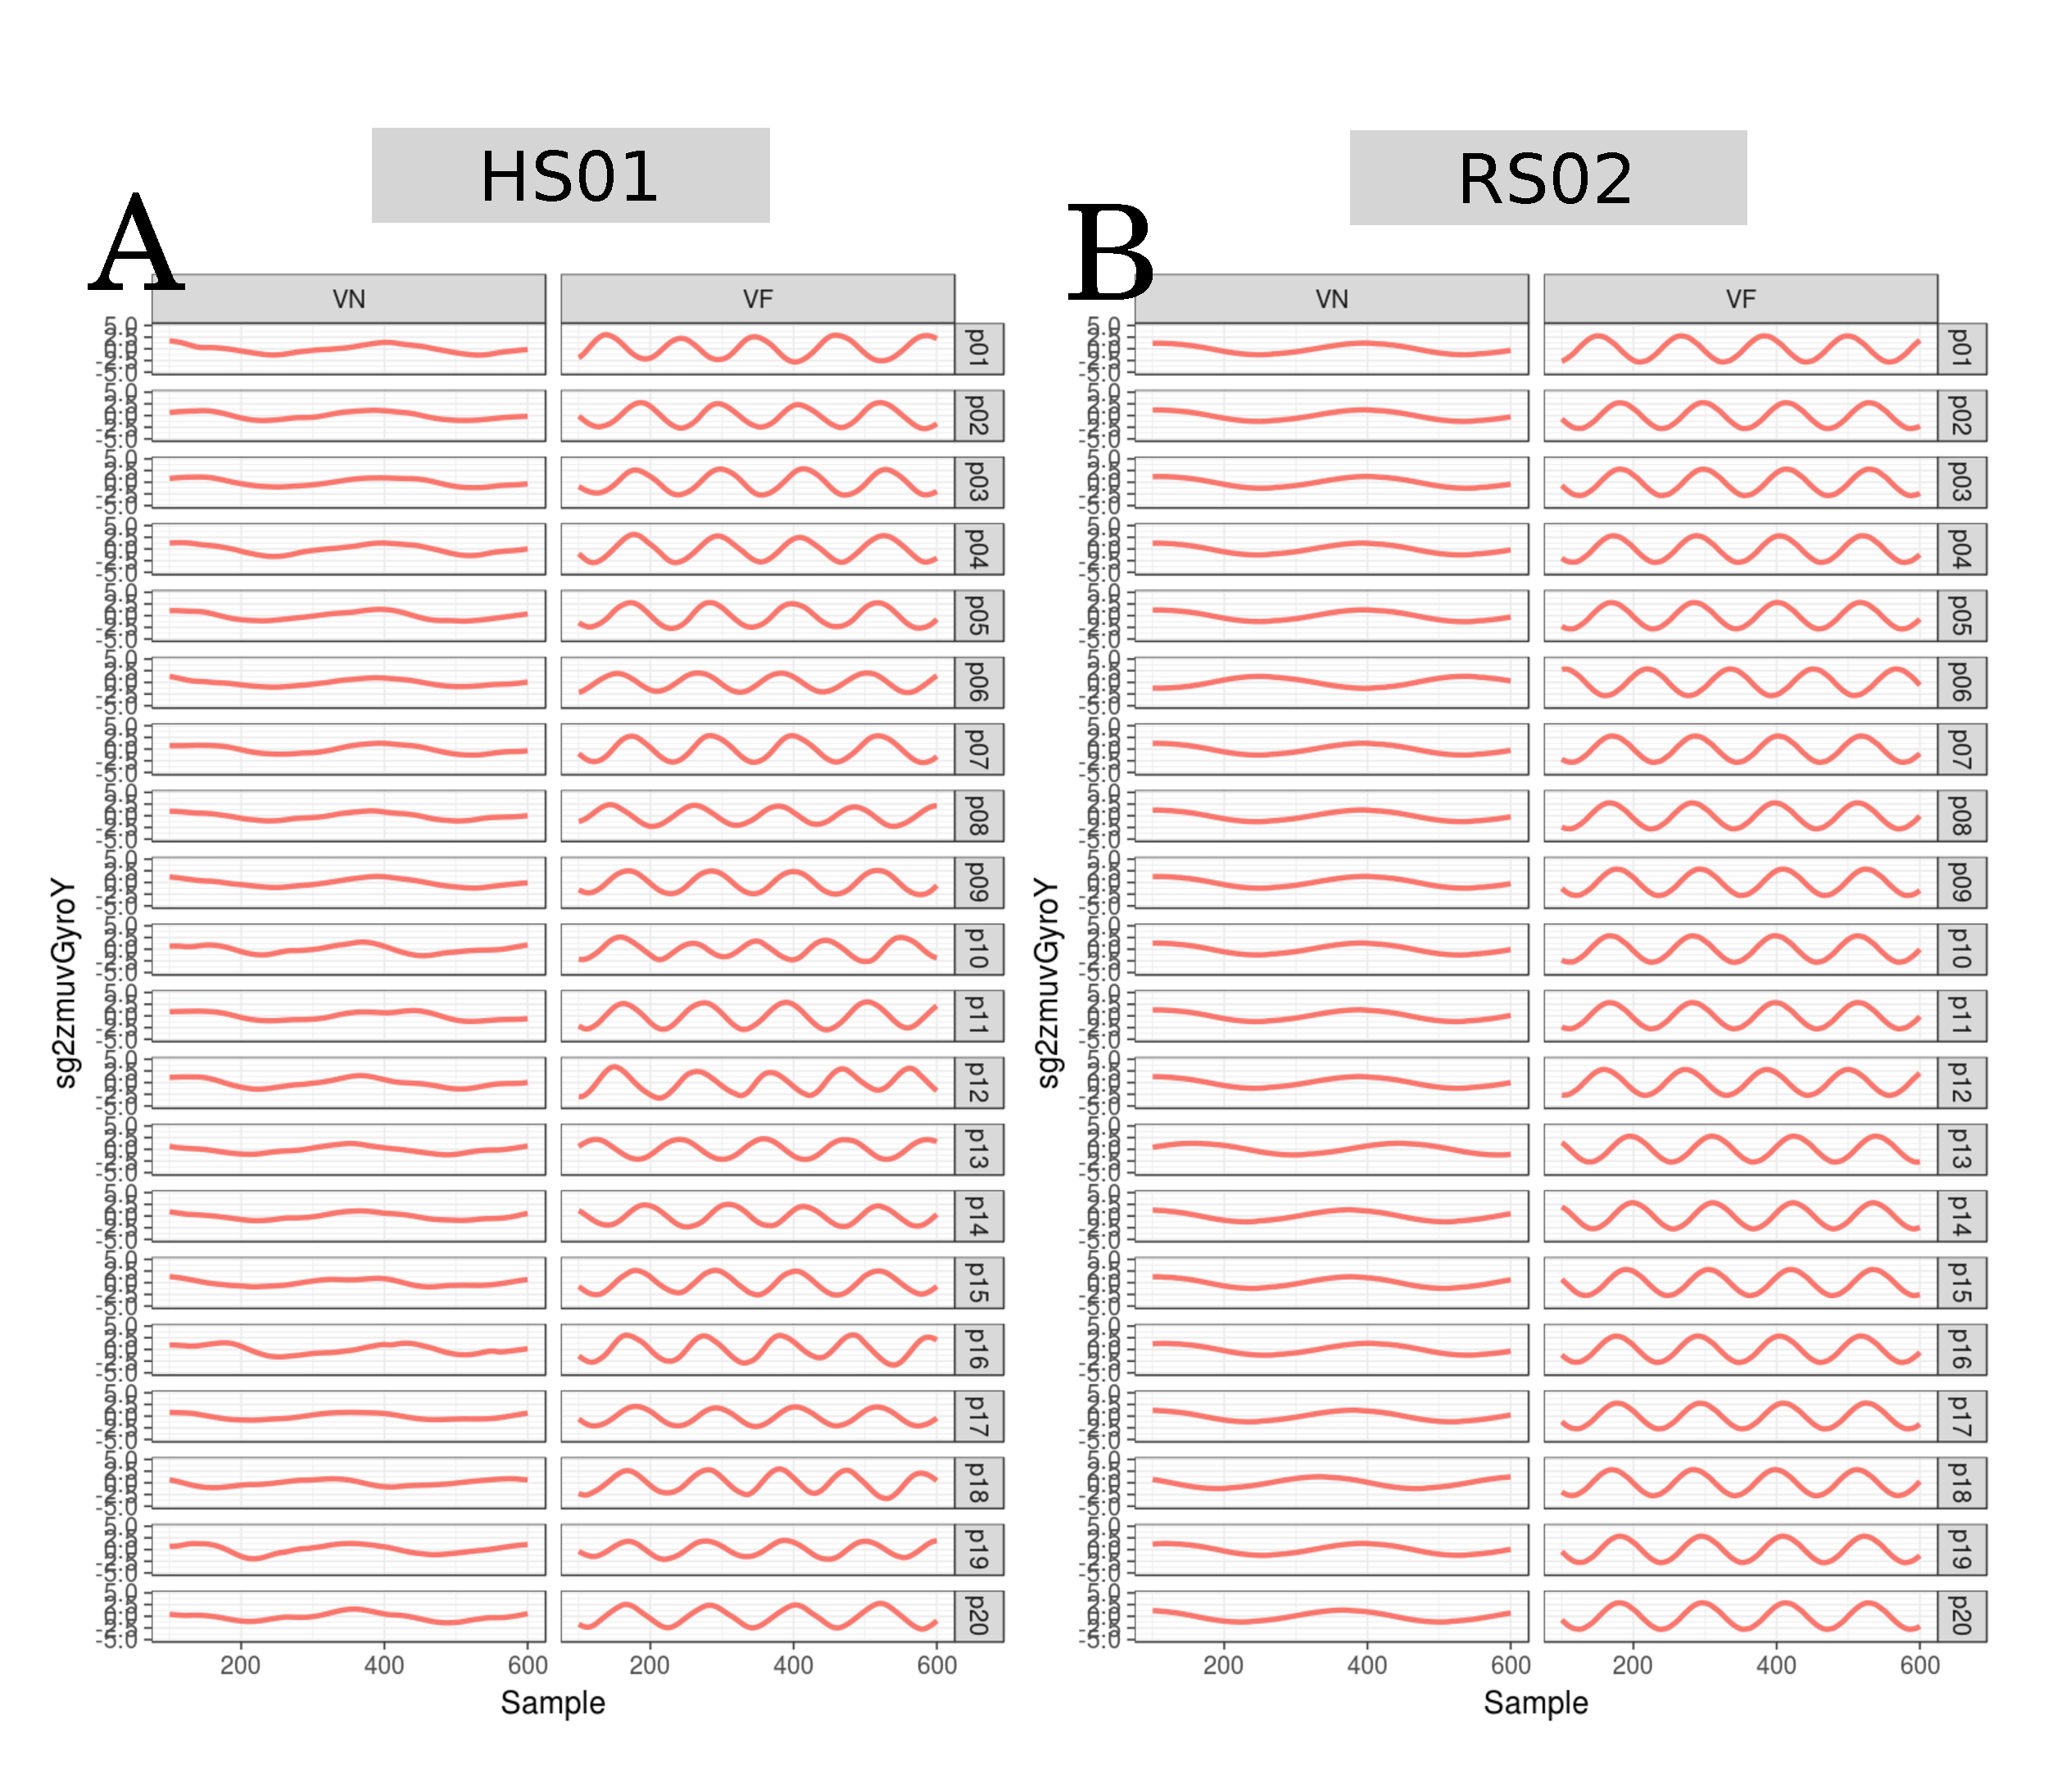
\includegraphics[width=1.0\textwidth]{aV-sg2}
    	\caption
	[Time series for vertical arm movements (sg2) ]{
	{\bf Time series for vertical arm movements (sg2)}
		Time series for sg0zmuvGyroY for twenty participants 
		($p01$ to  $p20$) 
		for vertical movements in normal (HN) and horizontal faster (HF) 
		velocity with sensors attached to the participant wrist (HS01)
		and to the humanoid wrist (RS02).
	R code to reproduce the figure is available from \cite{xochicale2018}.
        }
    \label{fig:aV-sg2}
\end{figure}
%%---------------------------------(FIGURE)-----------------------------------










\newpage
\section{Embedding parameters} \label{appendix:e:ep}
\subsection{Minimum dimension embedding values}

Minimum embedding dimensions for horizontal and vertical arm movements
are presented in Figs.  \ref{fig:caoH} and \ref{fig:caoV}, respectively.
For remained  results with window size lengths of time series data, we refer
the reader to download the data and code at \cite{xochicale2018}.


%%---------------------------------(FIGURE)-------------------------------------
%\begin{figure}[!h]
\begin{figure}
\centering
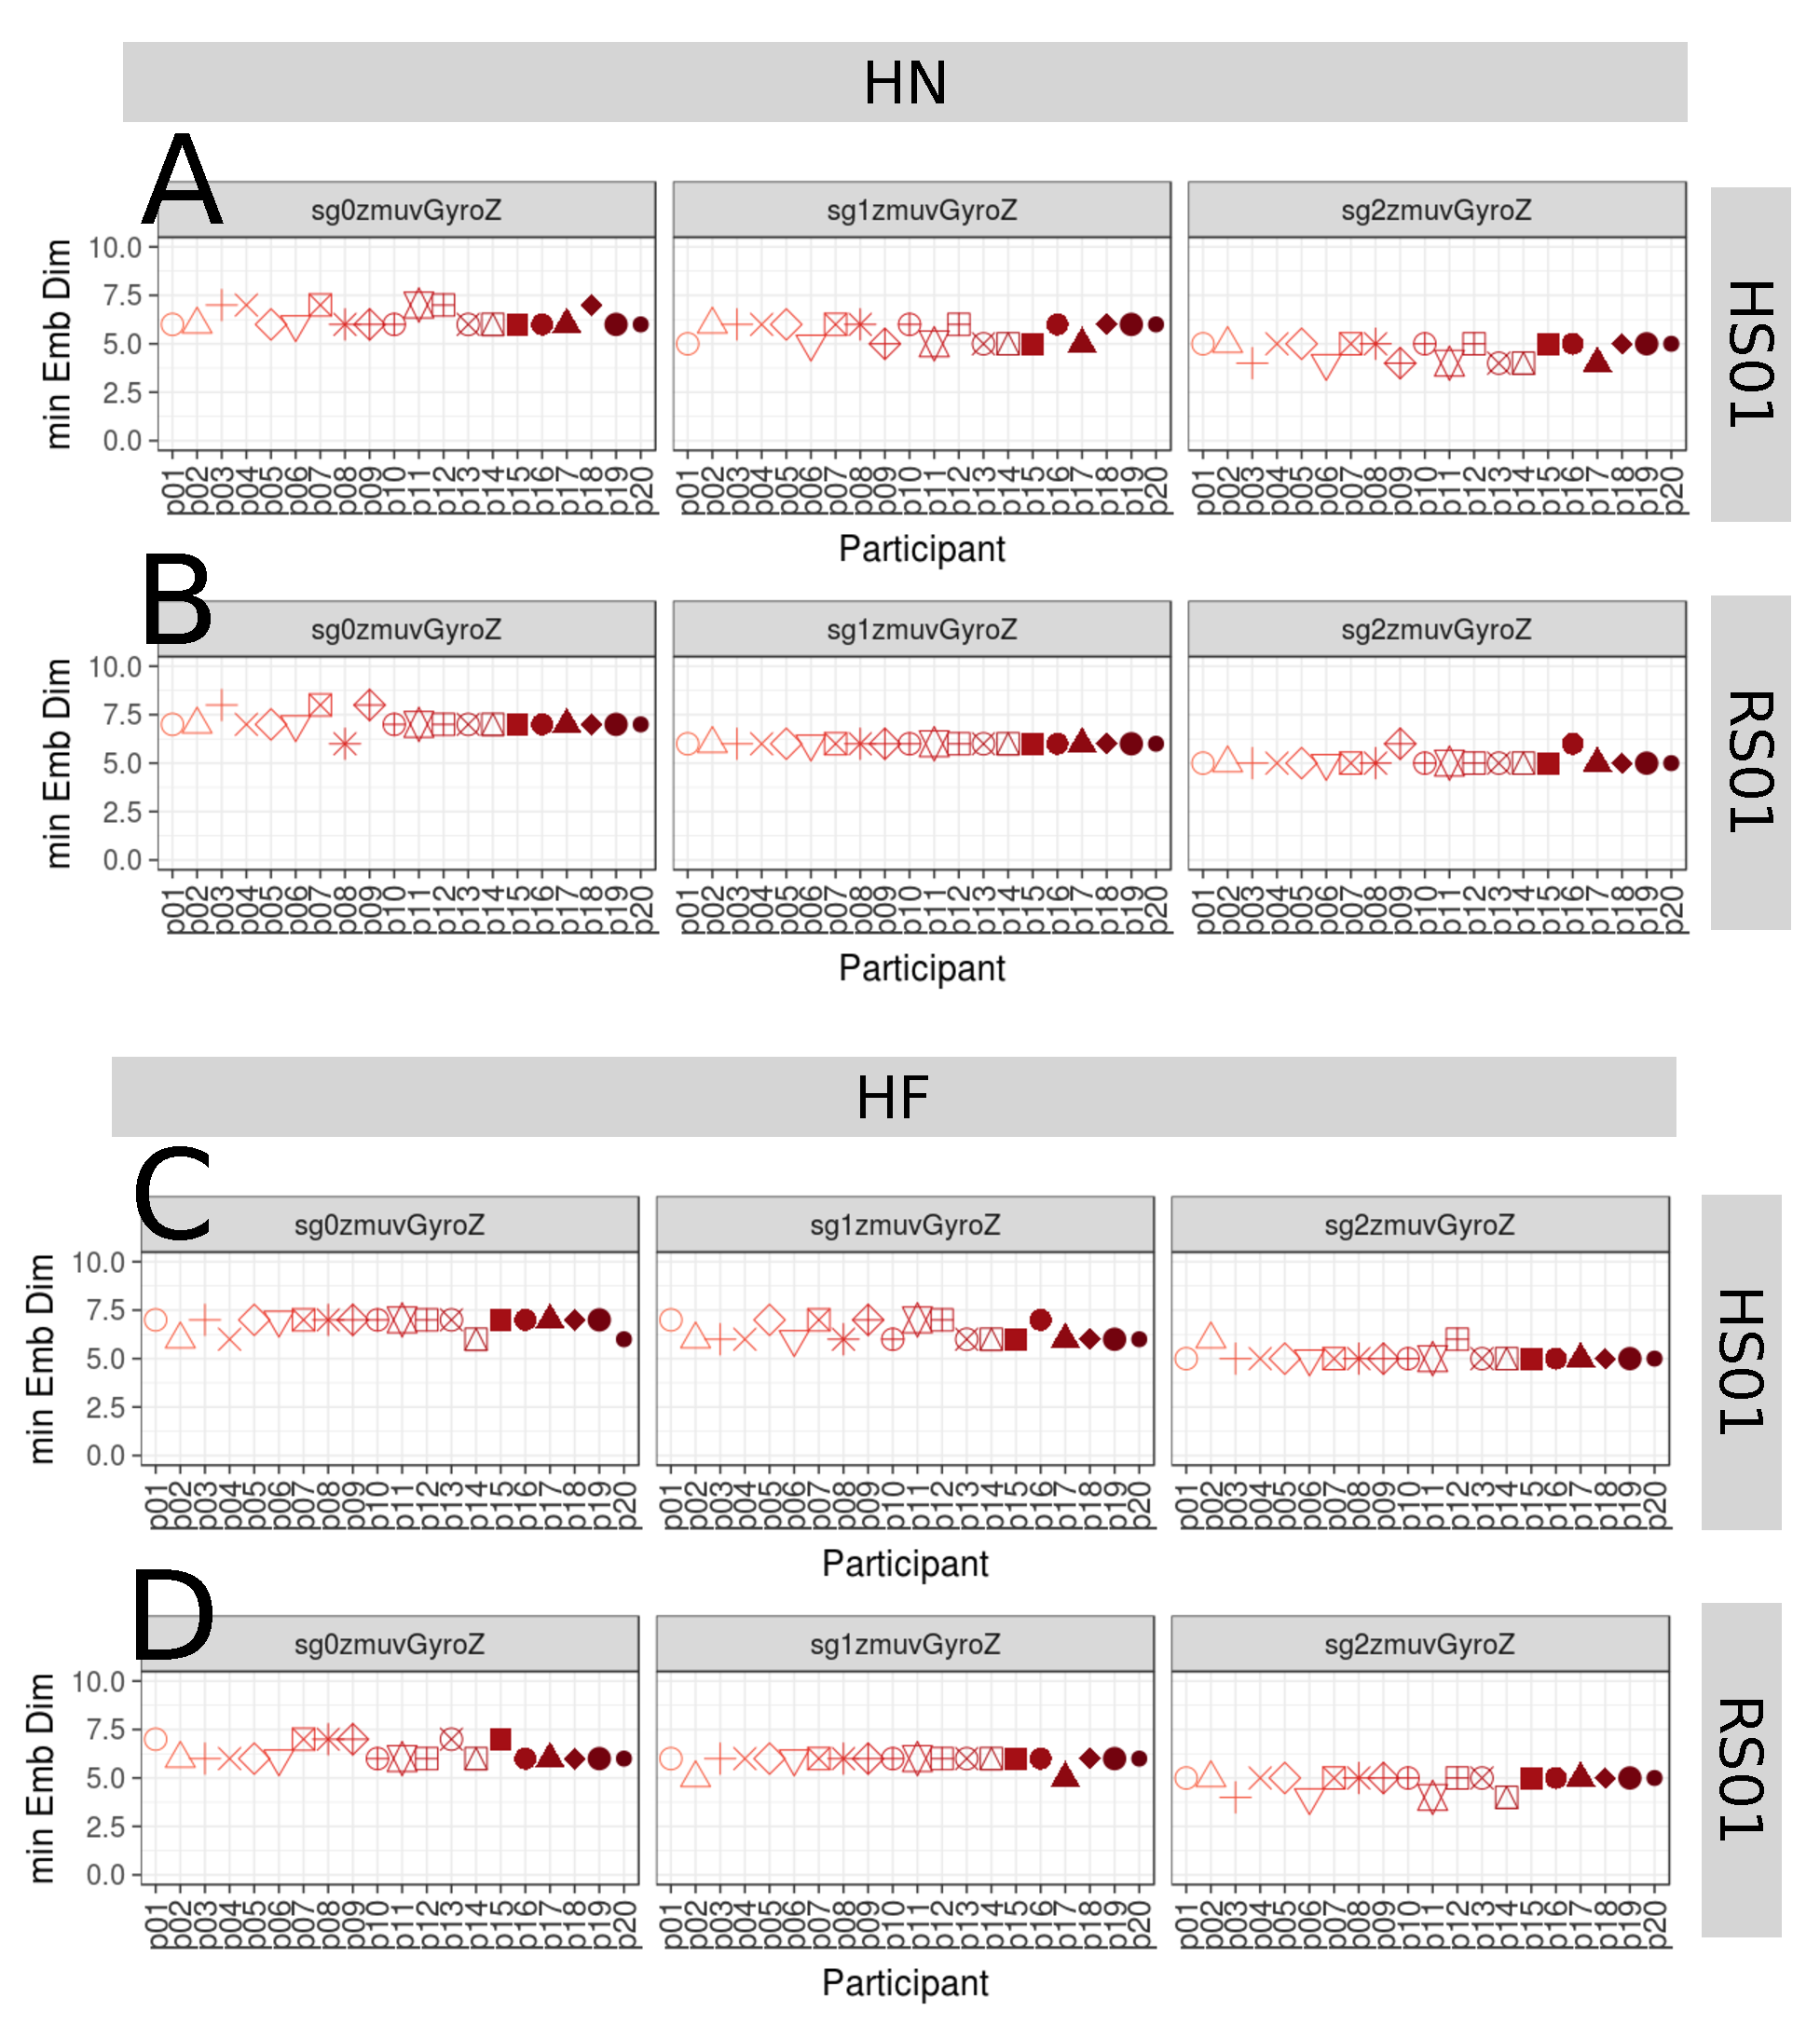
\includegraphics[width=1.0\textwidth]{cao_aHw10}
	\caption
	[Minimum embedding dimensions for horizontal arm movements]{
	{\bf Minimum embedding dimensions for horizontal arm movements.} 
		(A, B) Horizontal Normal (HN), (C, D) Horizontal Faster (HF) 
		movements,
		(A, C) sensor attached to participants (HS01), and
		(B, D) sensor attached to robot (RS01).
		Minimum embedding dimensions are for twenty participants 
		(p01 to p20) with three smoothed signals 
		(sg0zmuvGyroZ, sg1zmuvGyroZ and sg2zmuvGyroZ)
		and window lenght of 10-sec (500 samples).
		R code to reproduce the figure is available 
		from \cite{xochicale2018}.
        }
    \label{fig:caoH}
\end{figure}
%%---------------------------------(FIGURE)------------------------------------

%%---------------------------------(FIGURE)-------------------------------------
%\begin{figure}[!h]
\begin{figure}
\centering
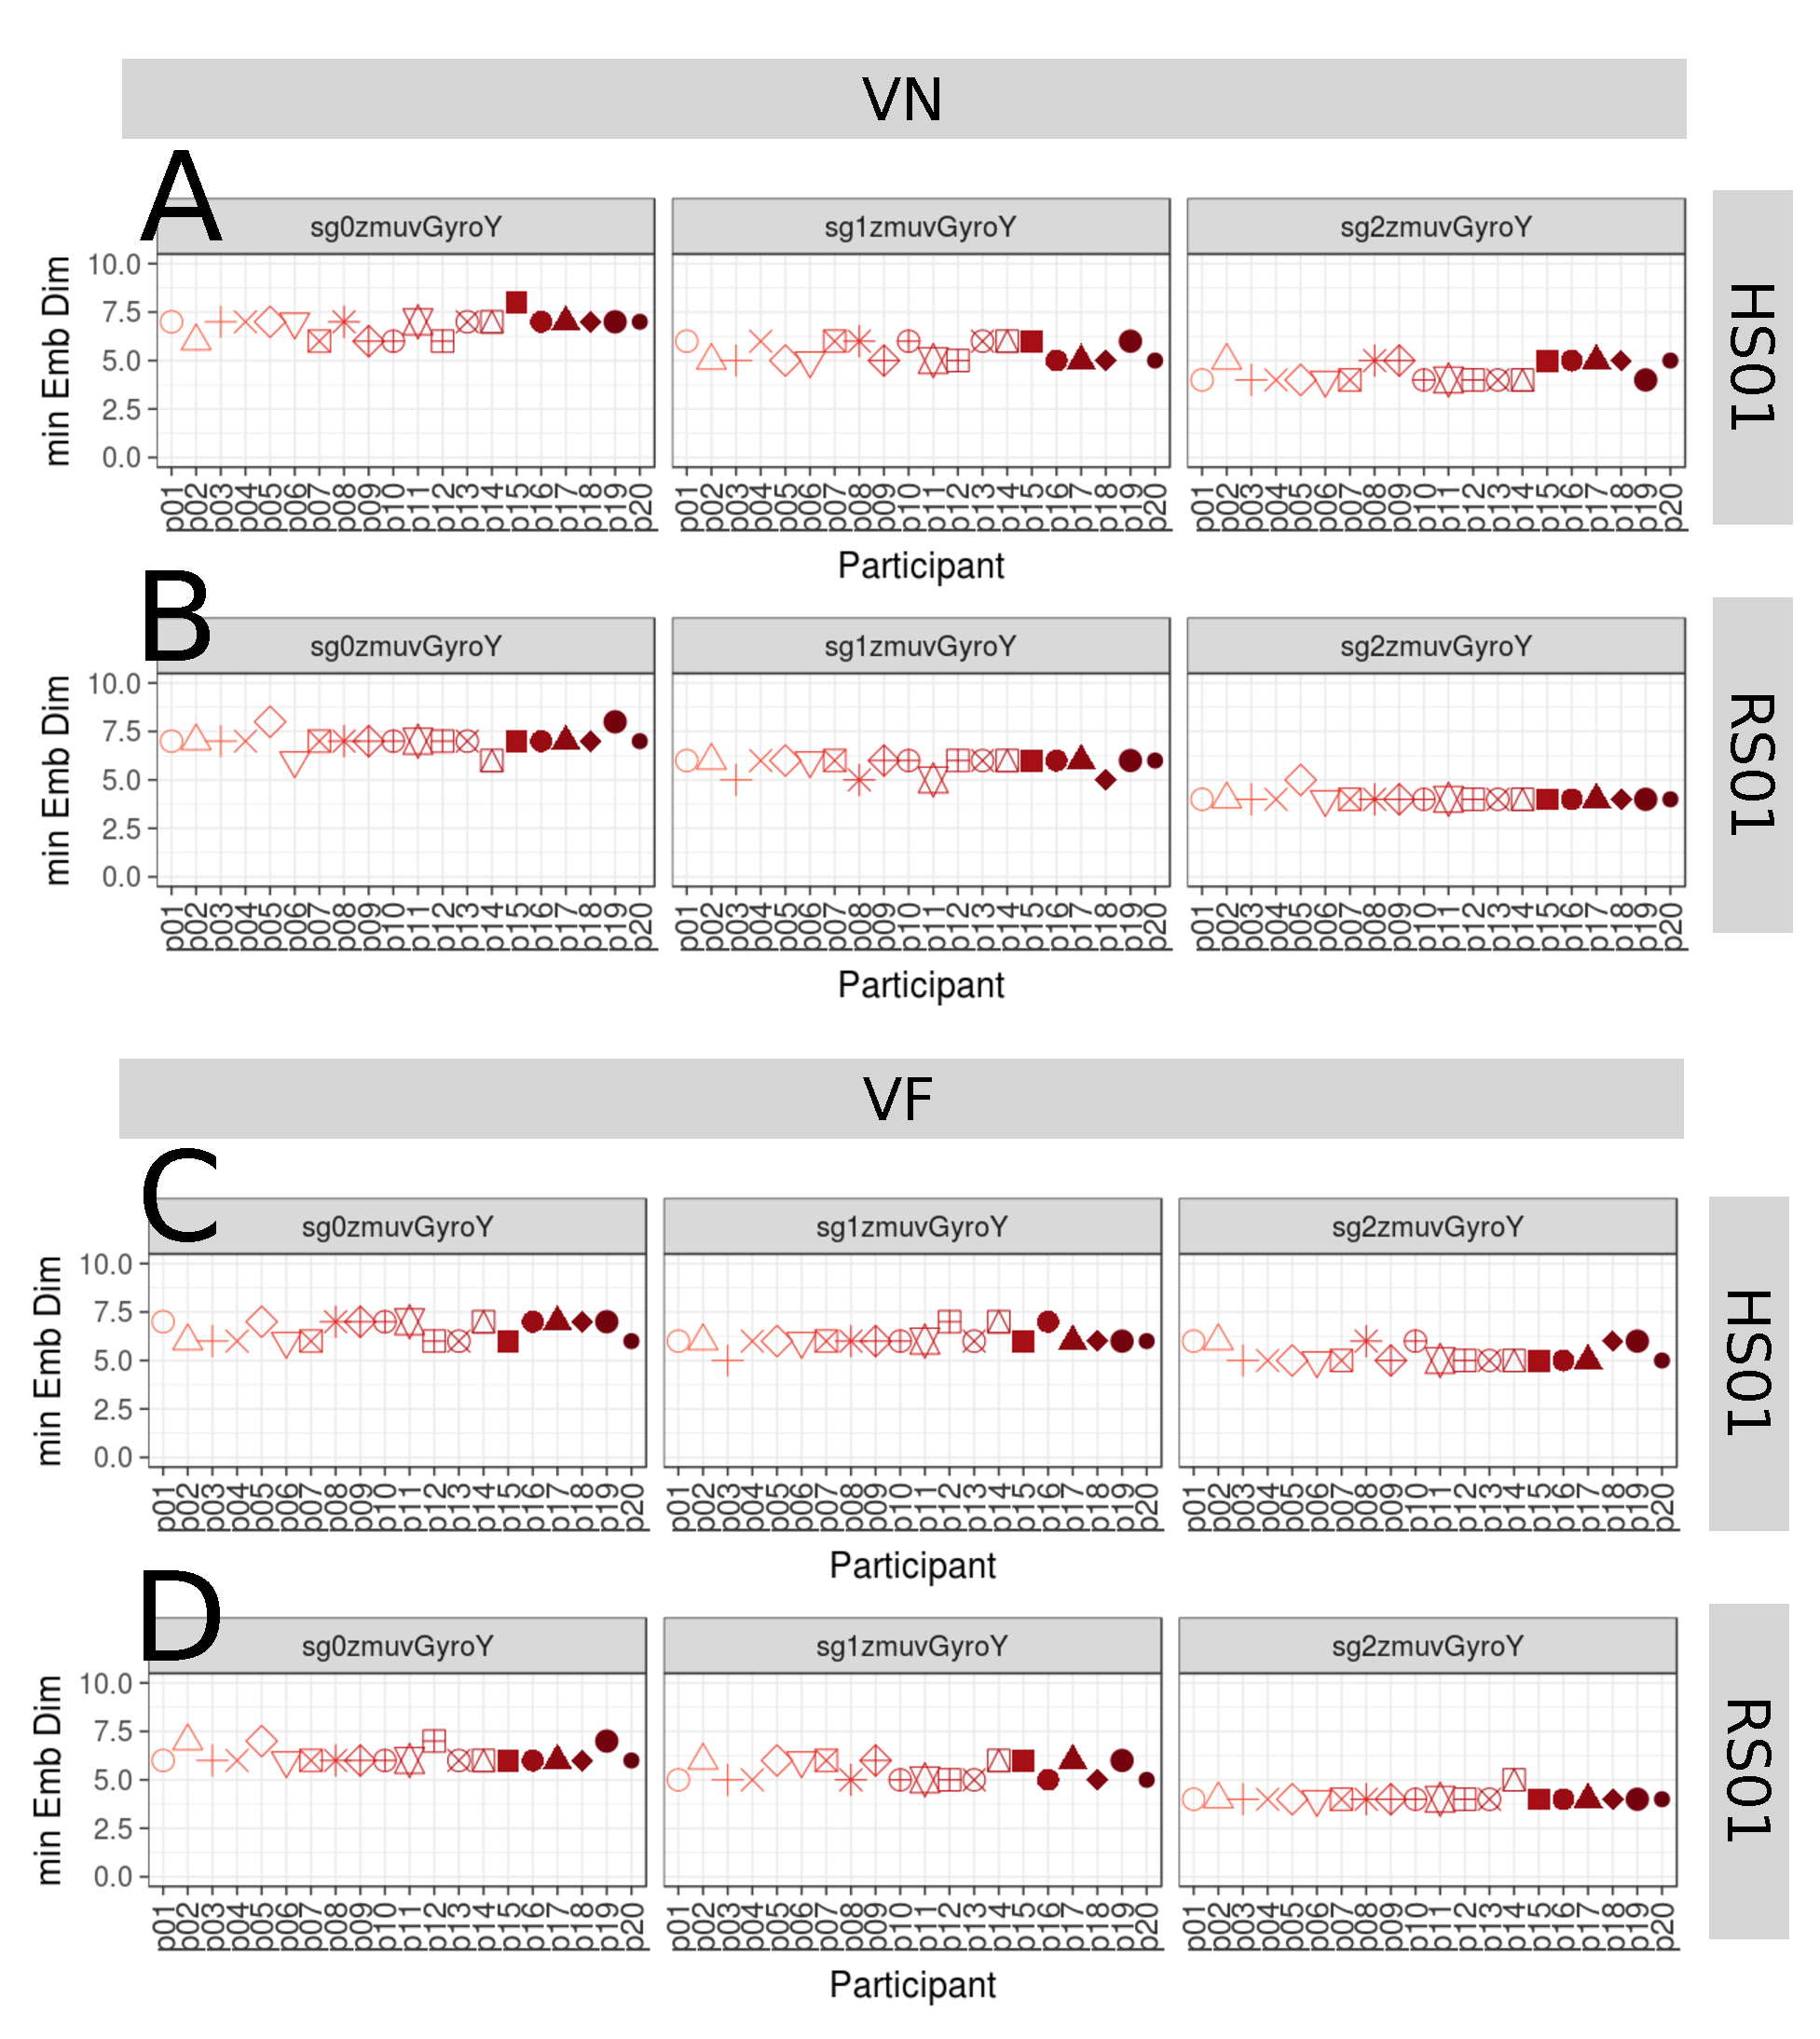
\includegraphics[width=1.0\textwidth]{cao_aVw10}
	\caption
	[Minimum embedding dimensions for vertical arm movements]{
	{\bf Minimum embedding dimensions for vertical arm movements.} 
		(A, B) Vertical Normal (VN), (C, D) Vertical Faster (VF) 
		movements,
		(A, C) sensor attached to participants (HS01), and		
		(B, D) sensor attached to robot (RS01).
		Minimum embedding dimensions are for twenty participants 
		(p01 to p20) with three smoothed signals (sg0zmuvGyroY, 
		sg1zmuvGyroY and sg2zmuvGyroY) 
		and window length of 10-sec (500 samples).
		R code to reproduce the figure is available 
		from \cite{xochicale2018}.
        }
    \label{fig:caoV}
\end{figure}
%%---------------------------------(FIGURE)------------------------------------


\newpage
\subsection{Minimum delay embedding values}
First minimum AMI values for horizontal and vertical arm movements
are presented in Figs.  \ref{fig:amiH} and \ref{fig:amiV}, respectively.
For remained  results with window size lengths of time series data, we refer
the reader to download the data and code at \cite{xochicale2018}.

%%---------------------------------(FIGURE)-------------------------------------
%\begin{figure}[!h]
\begin{figure}
\centering
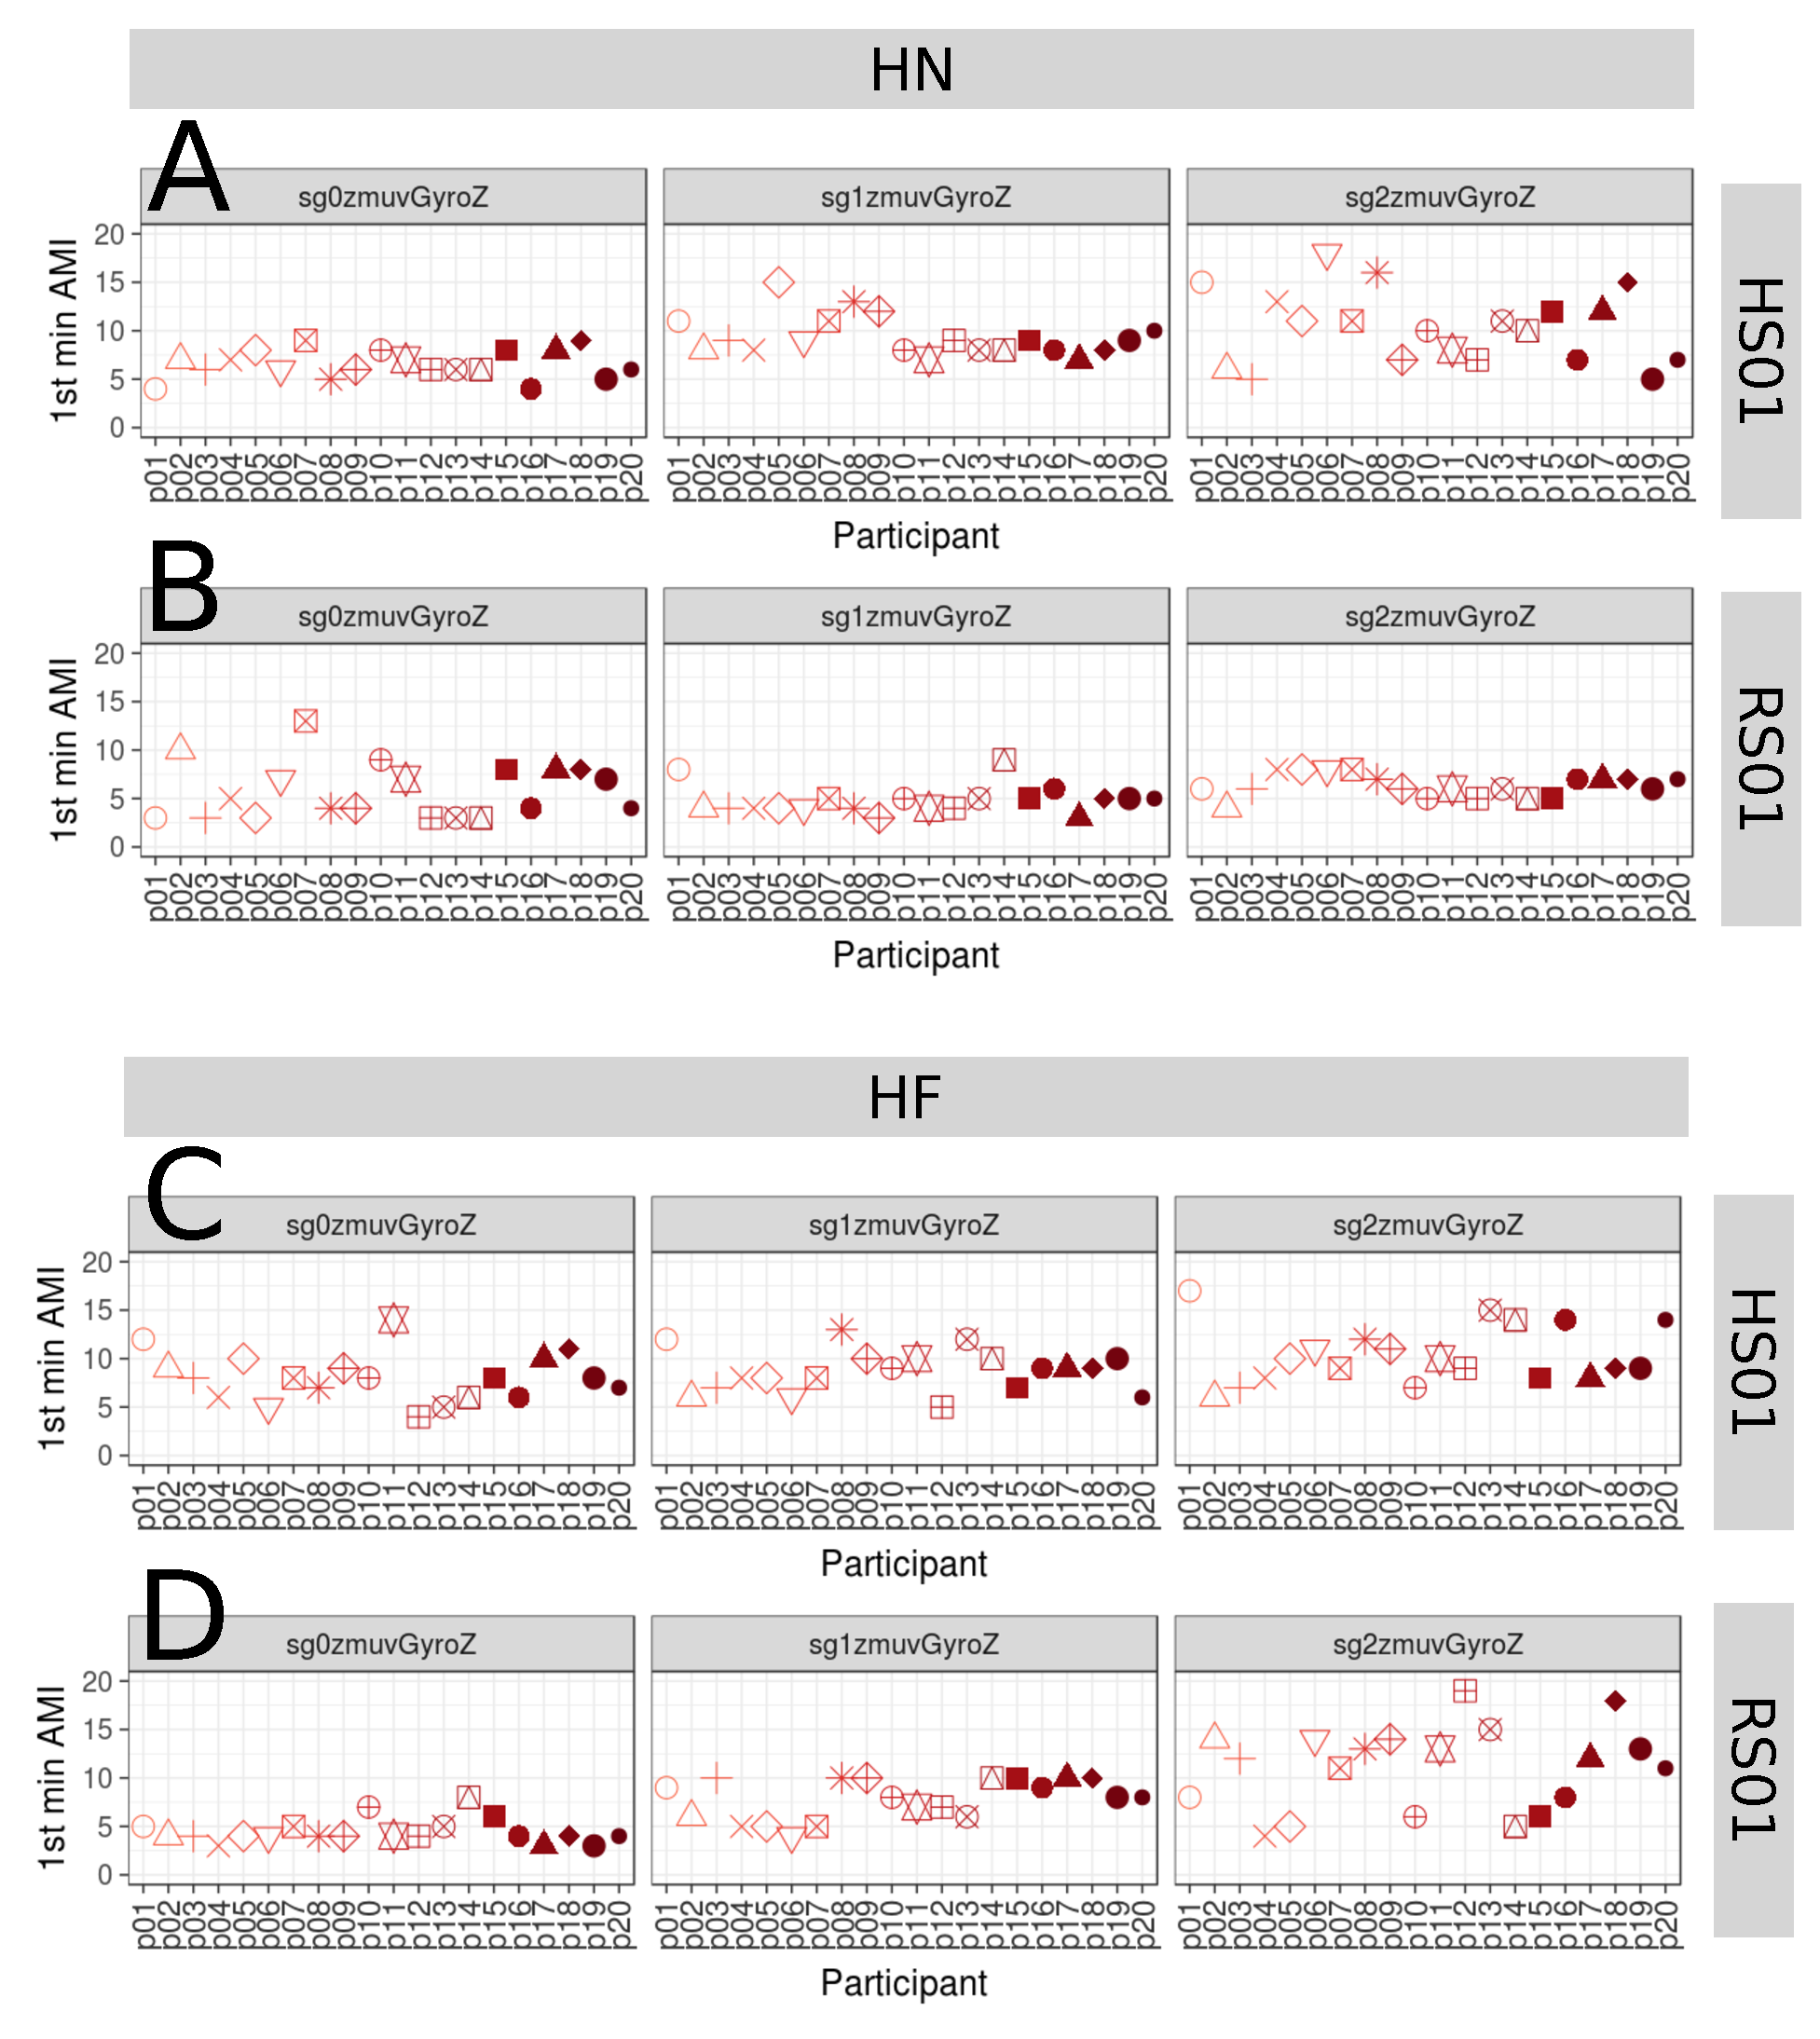
\includegraphics[width=1.0\textwidth]{ami_aHw10}
	\caption
	[First minimum AMI values for horizontal arm movements]{
	{\bf First minimum AMI values for horizontal arm movements.}
		(A, B) Horizontal Normal (HN), (C, D) Horizontal Faster (HF) 
		movements,
		(A, C) sensor attached to participants (HS01), and
		(B, D) sensor attached to robot (RS01).
		First minimum AMI values are for twenty participants 
		(p01 to p20) with three smoothed signals (sg0zmuvGyroZ, 
		sg1zmuvGyroZ and sg2zmuvGyroZ) and  window lenght of 
		10-sec (500 samples).
		R code to reproduce the figure is available 
		from \cite{xochicale2018}.
        }
    \label{fig:amiH}
\end{figure}
%%---------------------------------(FIGURE)------------------------------------

%%---------------------------------(FIGURE)-------------------------------------
%\begin{figure}[!h]
\begin{figure}
\centering
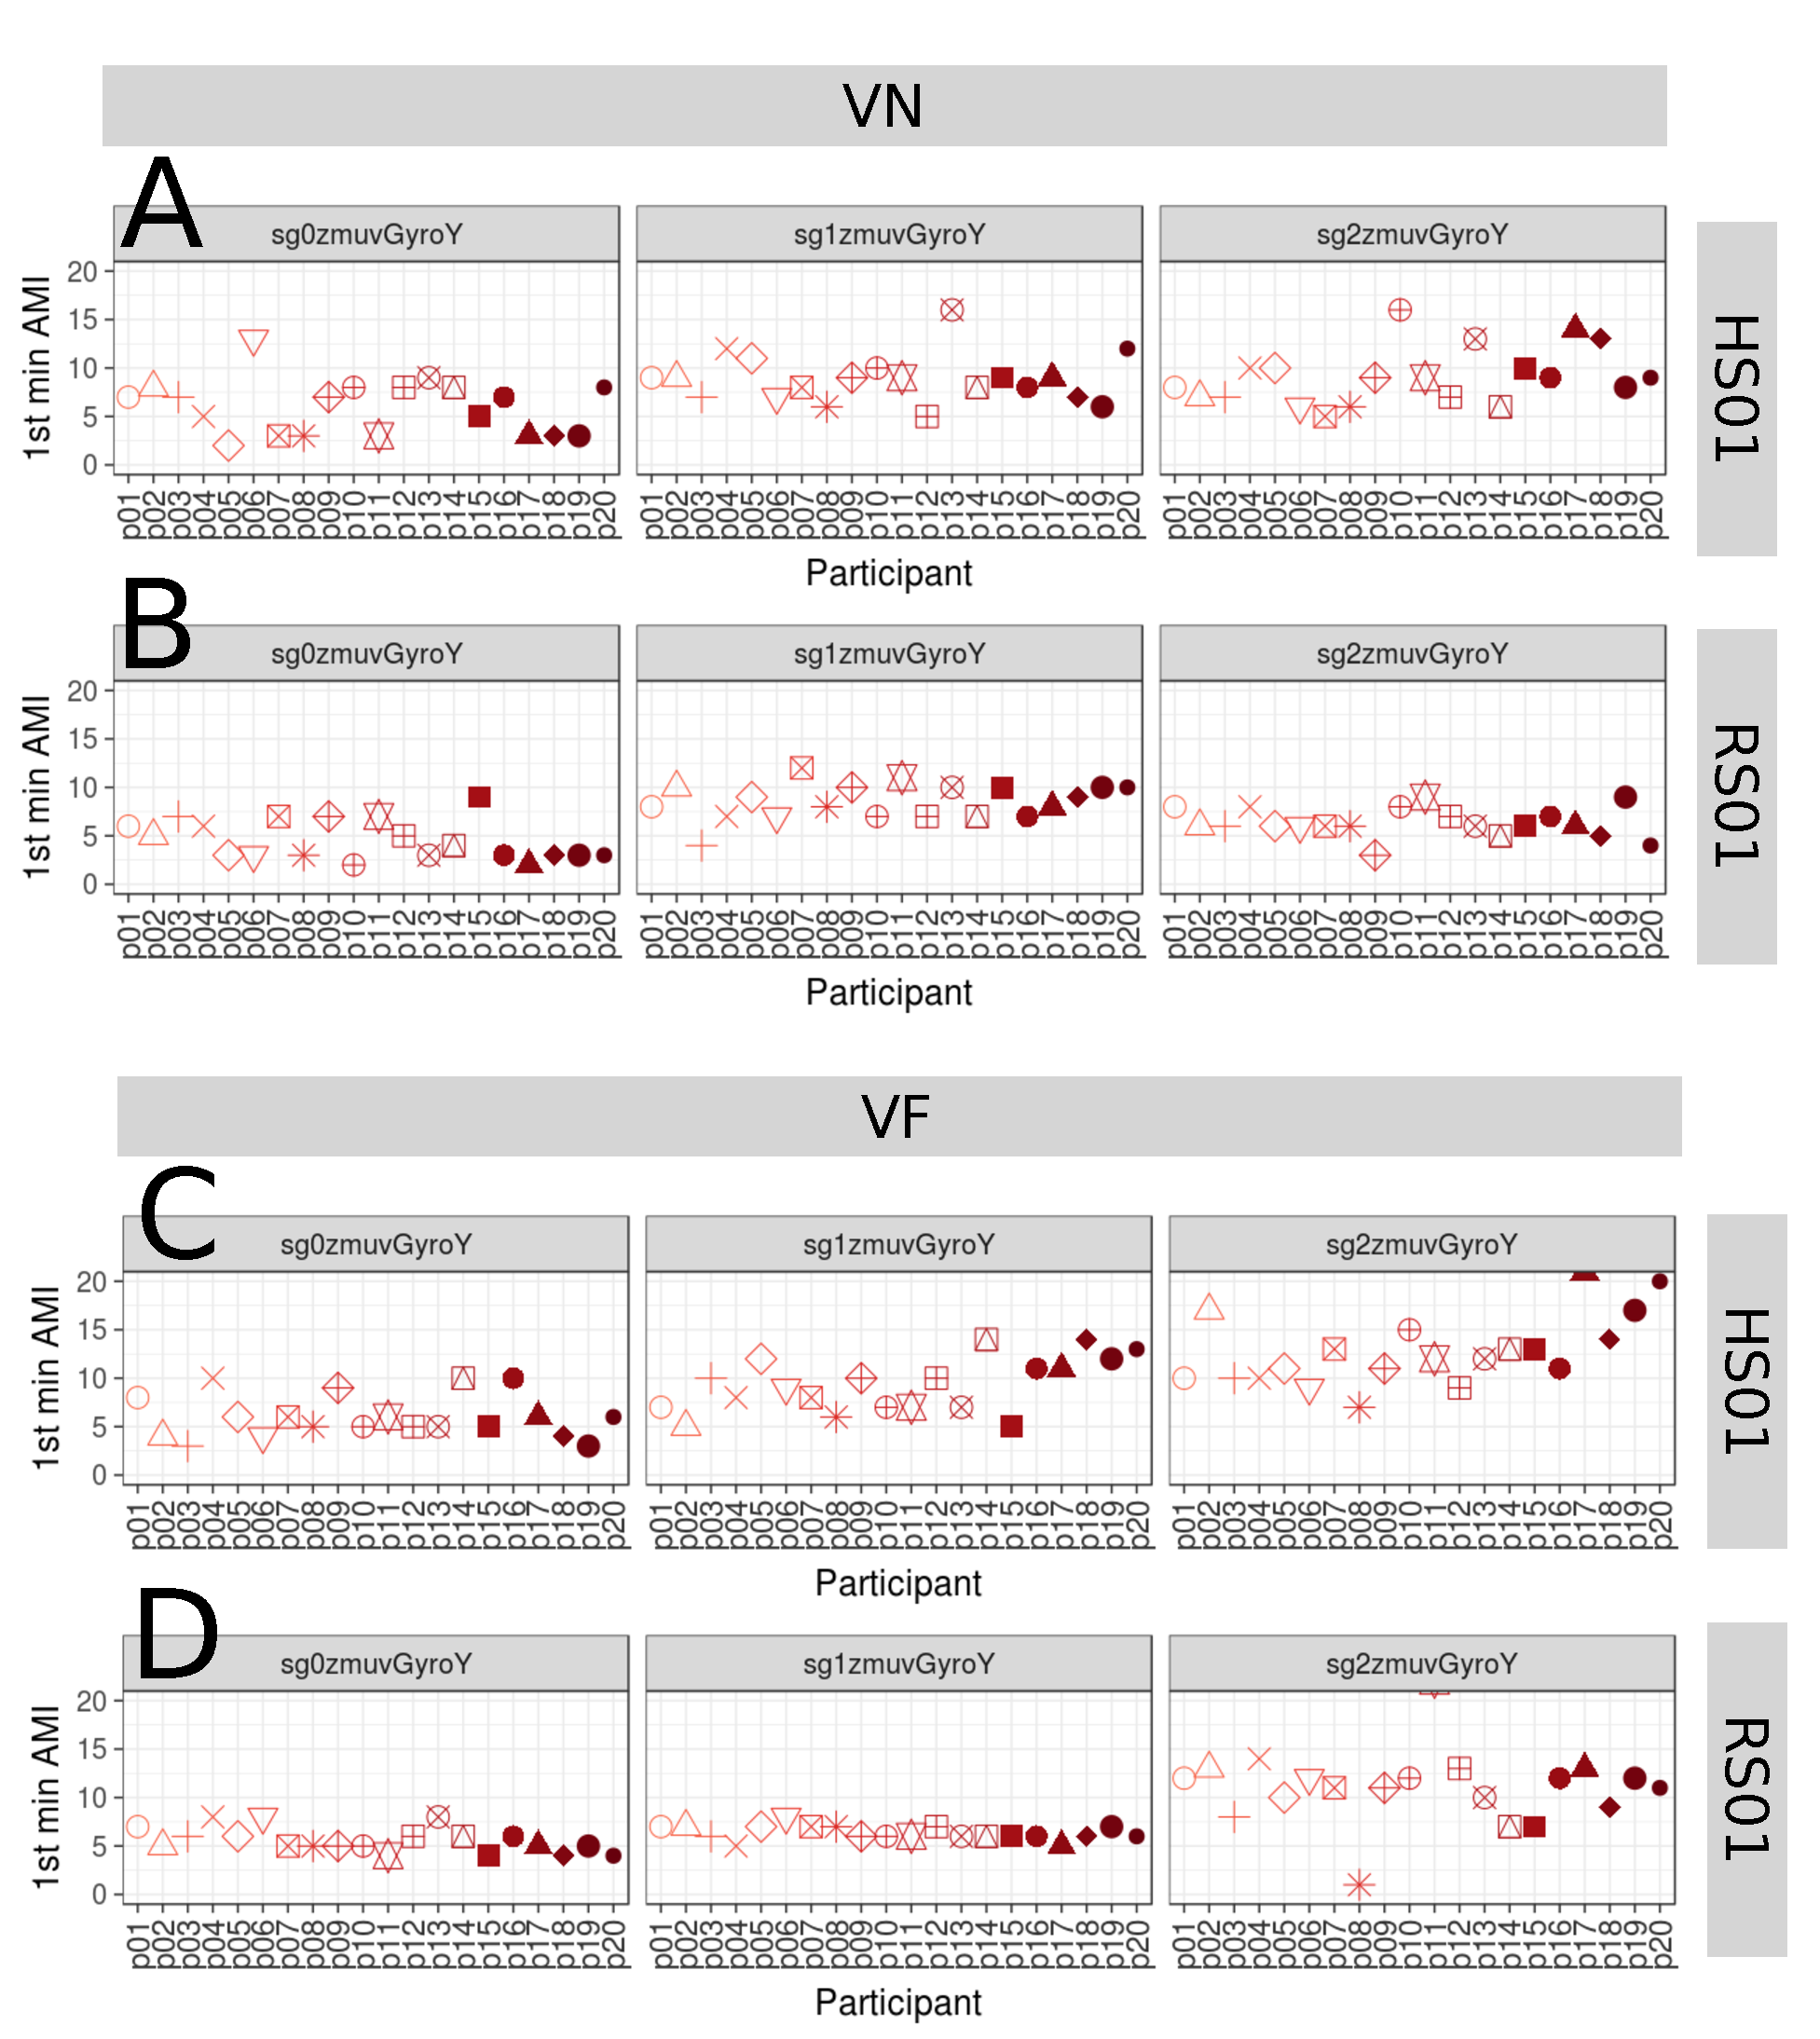
\includegraphics[width=1.0\textwidth]{ami_aVw10}
	\caption
	[First minimum AMI values for vertical arm movements]{
	{\bf First minimum AMI values for vertical arm movements.}
		(A, B) Vertical Normal (VN), (C, D) Vertical Faster (VF) 
		movements,
		(A, C) sensor attached to participants (HS01), and
		(B, D) sensor attached to robot (RS01).
		First minimum AMI values are for twenty participants 
		(p01 to p20) with three smoothed signals (sg0zmuvGyroZ, 
		sg1zmuvGyroZ and sg2zmuvGyroZ) and  window lenght of 
		10-sec (500 samples).
		R code to reproduce the figure is available 
		from \cite{xochicale2018}.
        }
    \label{fig:amiV}
\end{figure}
%%---------------------------------(FIGURE)------------------------------------




\newpage
\section{RSSs} \label{appendix:e:rsss}

Reconstructed state spaces of participant $p01$, $p02$ and $p03$ 
for horizontal arm movements (Figs. \ref{fig:rss_HN} and \ref{fig:rss_HF})
and vertical arm movements  (Figs. \ref{fig:rss_VN} and \ref{fig:rss_VF}).
For remained  results with window size lengths of time series data, we refer
the reader to download the data and code at \cite{xochicale2018}.



%%---------------------------------(FIGURE)-------------------------------------
\begin{figure}
\centering
\includegraphics[height=0.85\textheight]{rss_HN}
\caption
	[RSSs for horizontal normal arm movements]{
	{\bf RSSs for horizontal normal arm movements.}
	Reconstructed state spaces %for time series of Figure \ref{fig:tsH}.
	of participant $p01$, $p02$ and $p03$ for horizontal movements 
	with raw-normalised (sg0zmuvGyroZ), 
	normalised-smoothed 1 (sg1zmuvGyroZ) and 
	normalised-smoothed 2 (sg2zmuvGyroZ) time series of the 
	sensors attached to the participant (HS01) and other sensor 
	attached to the robot (RS01).	
	Reconstructed state spaces were computed with 
	embedding parameters $m=6$, $\tau=8$.
	R code to reproduce the figure is available from \cite{xochicale2018}.
        }
    \label{fig:rss_HN}
\end{figure}
%%---------------------------------(FIGURE)------------------------------------

%%---------------------------------(FIGURE)-------------------------------------
\begin{figure}
\centering
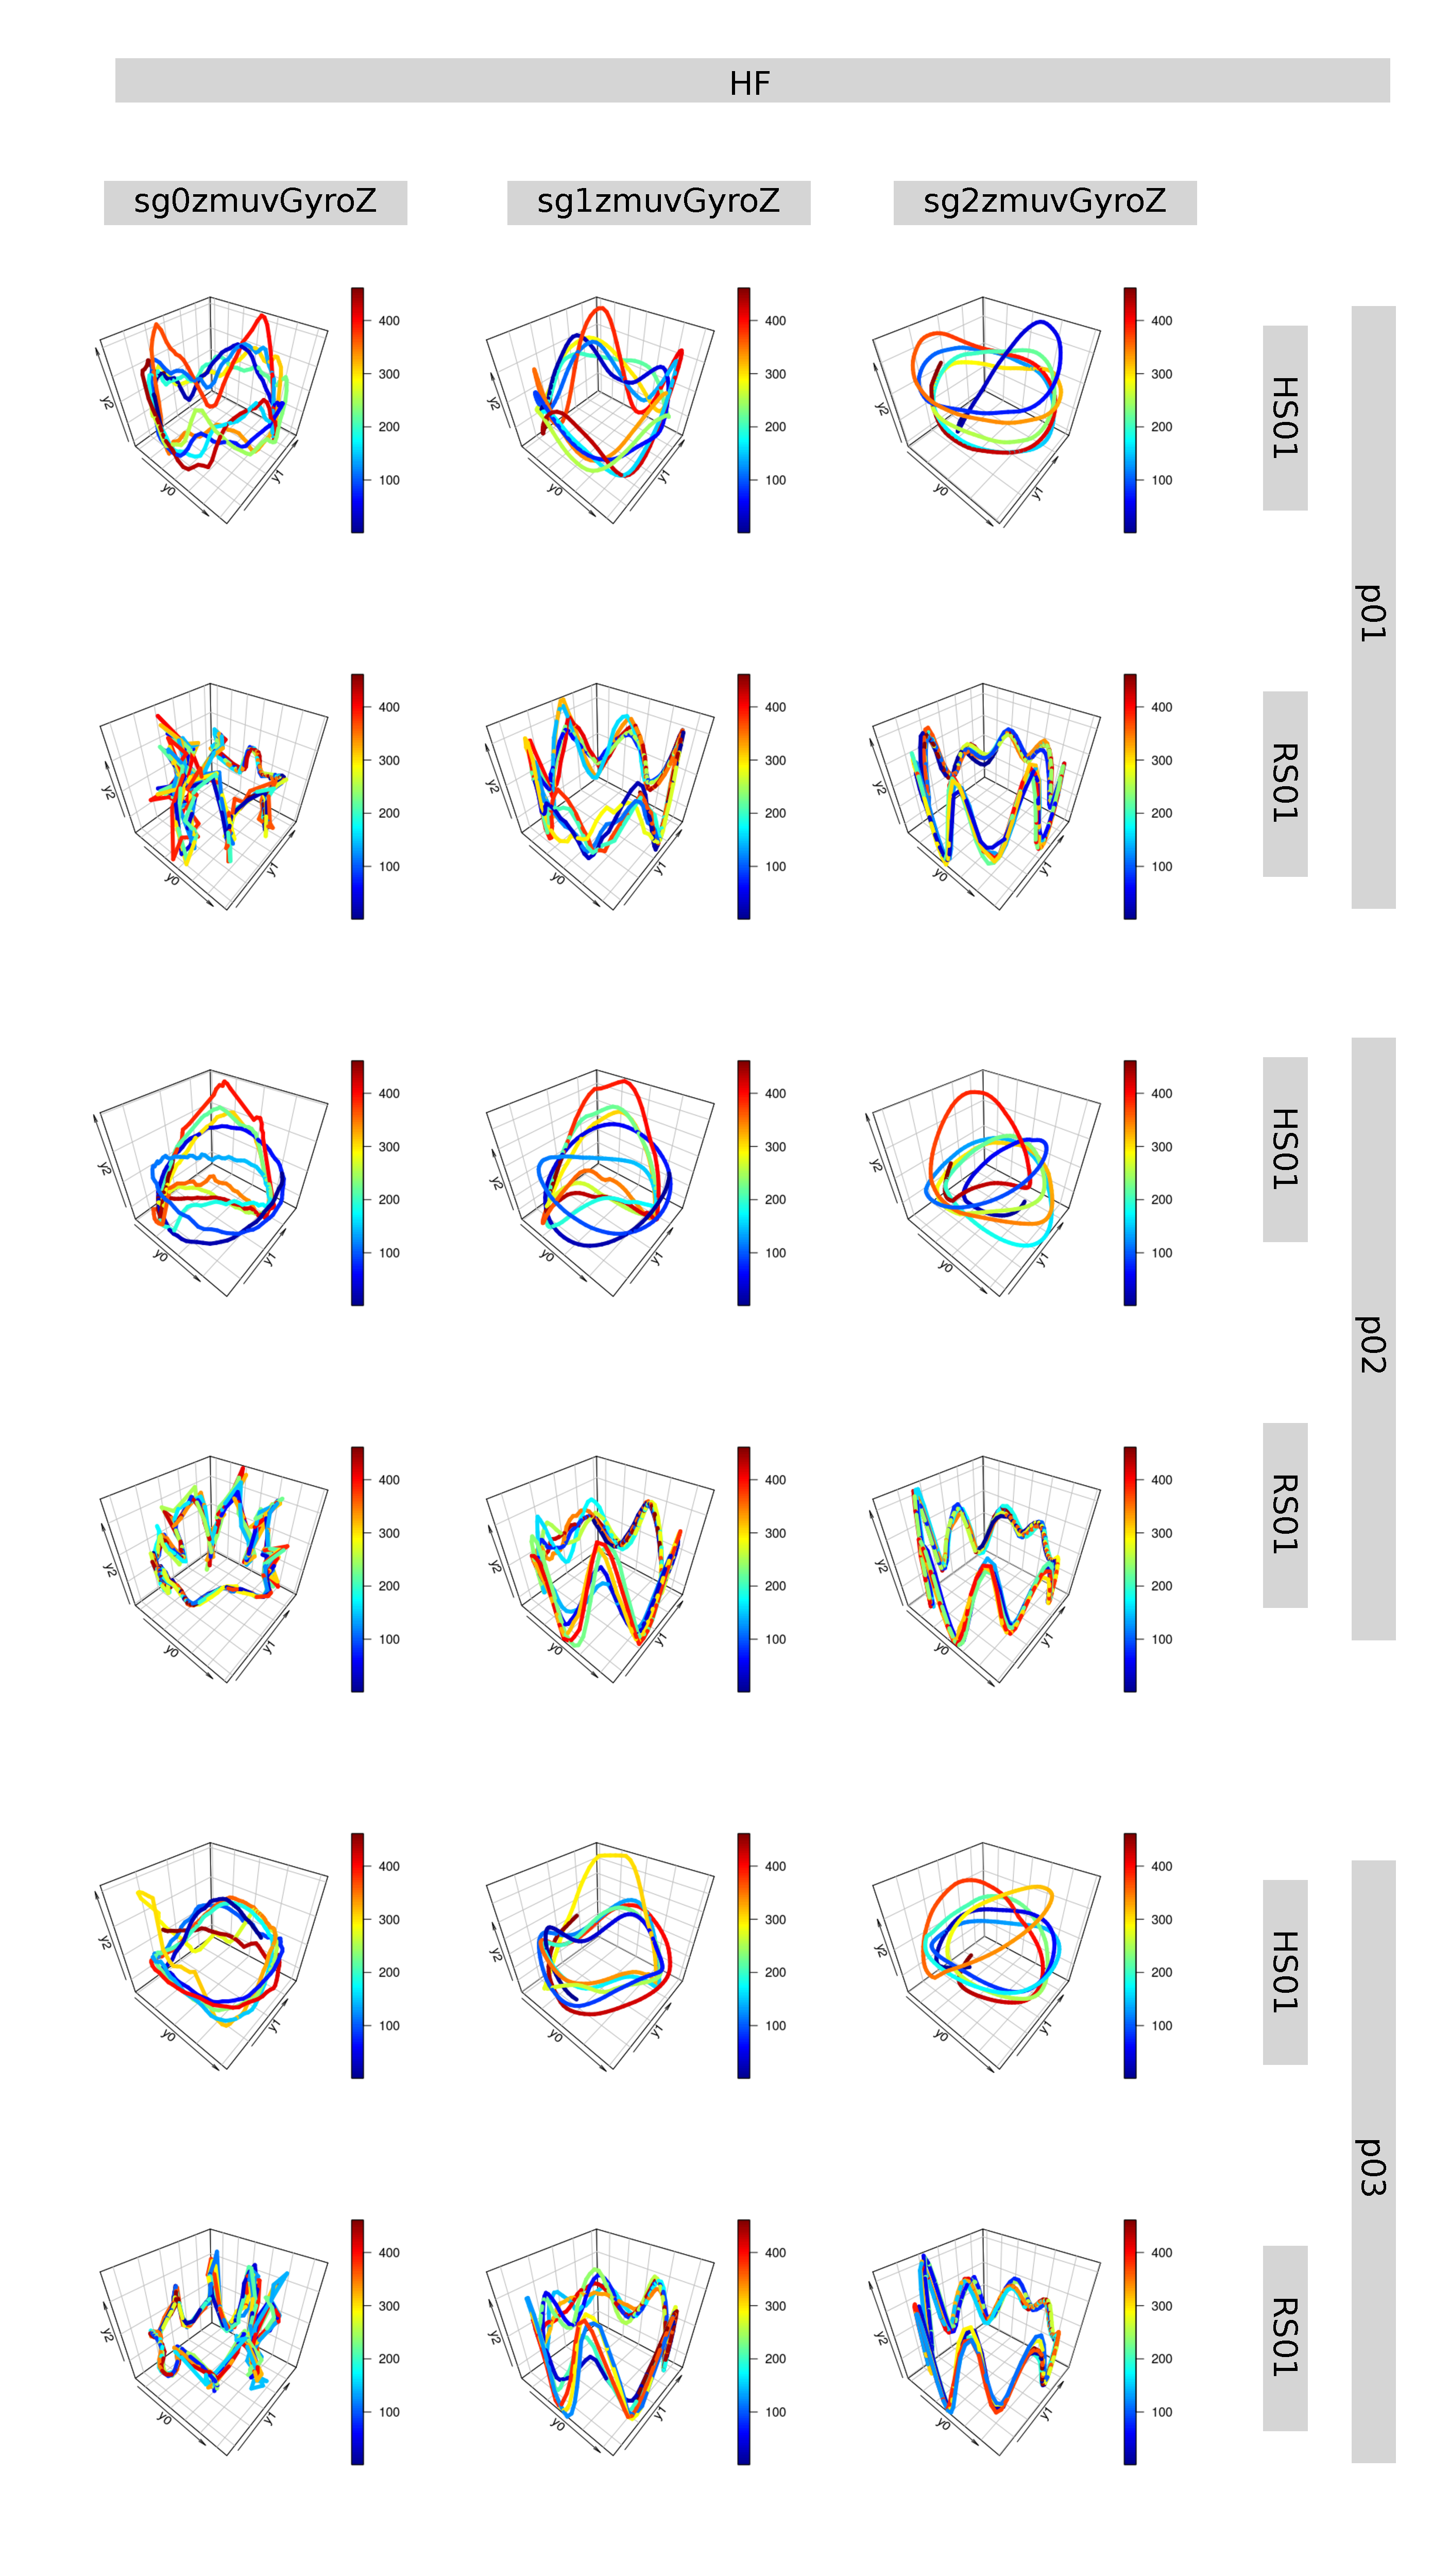
\includegraphics[height=0.85\textheight]{rss_HF}
\caption
	[RSSs for horizontal faster arm movements]{
	{\bf RSSs for horizontal faster arm movements.}
	Reconstructed state spaces %for time series of Figure \ref{fig:tsH}.
	of participant $p01$, $p02$ and $p03$ for horizontal faster movements 
	with raw-normalised (sg0zmuvGyroZ), 
	normalised-smoothed 1 (sg1zmuvGyroZ) and 
	normalised-smoothed 2 (sg2zmuvGyroZ) time series of the 
	sensors attached to the participant (HS01) and other sensor 
	attached to the robot (RS01).	
	Reconstructed state spaces were computed with 
	embedding parameters $m=6$, $\tau=8$.
	R code to reproduce the figure is available from \cite{xochicale2018}.
        }
    \label{fig:rss_HF}
\end{figure}
%%---------------------------------(FIGURE)------------------------------------



%%---------------------------------(FIGURE)-------------------------------------
\begin{figure}
\centering
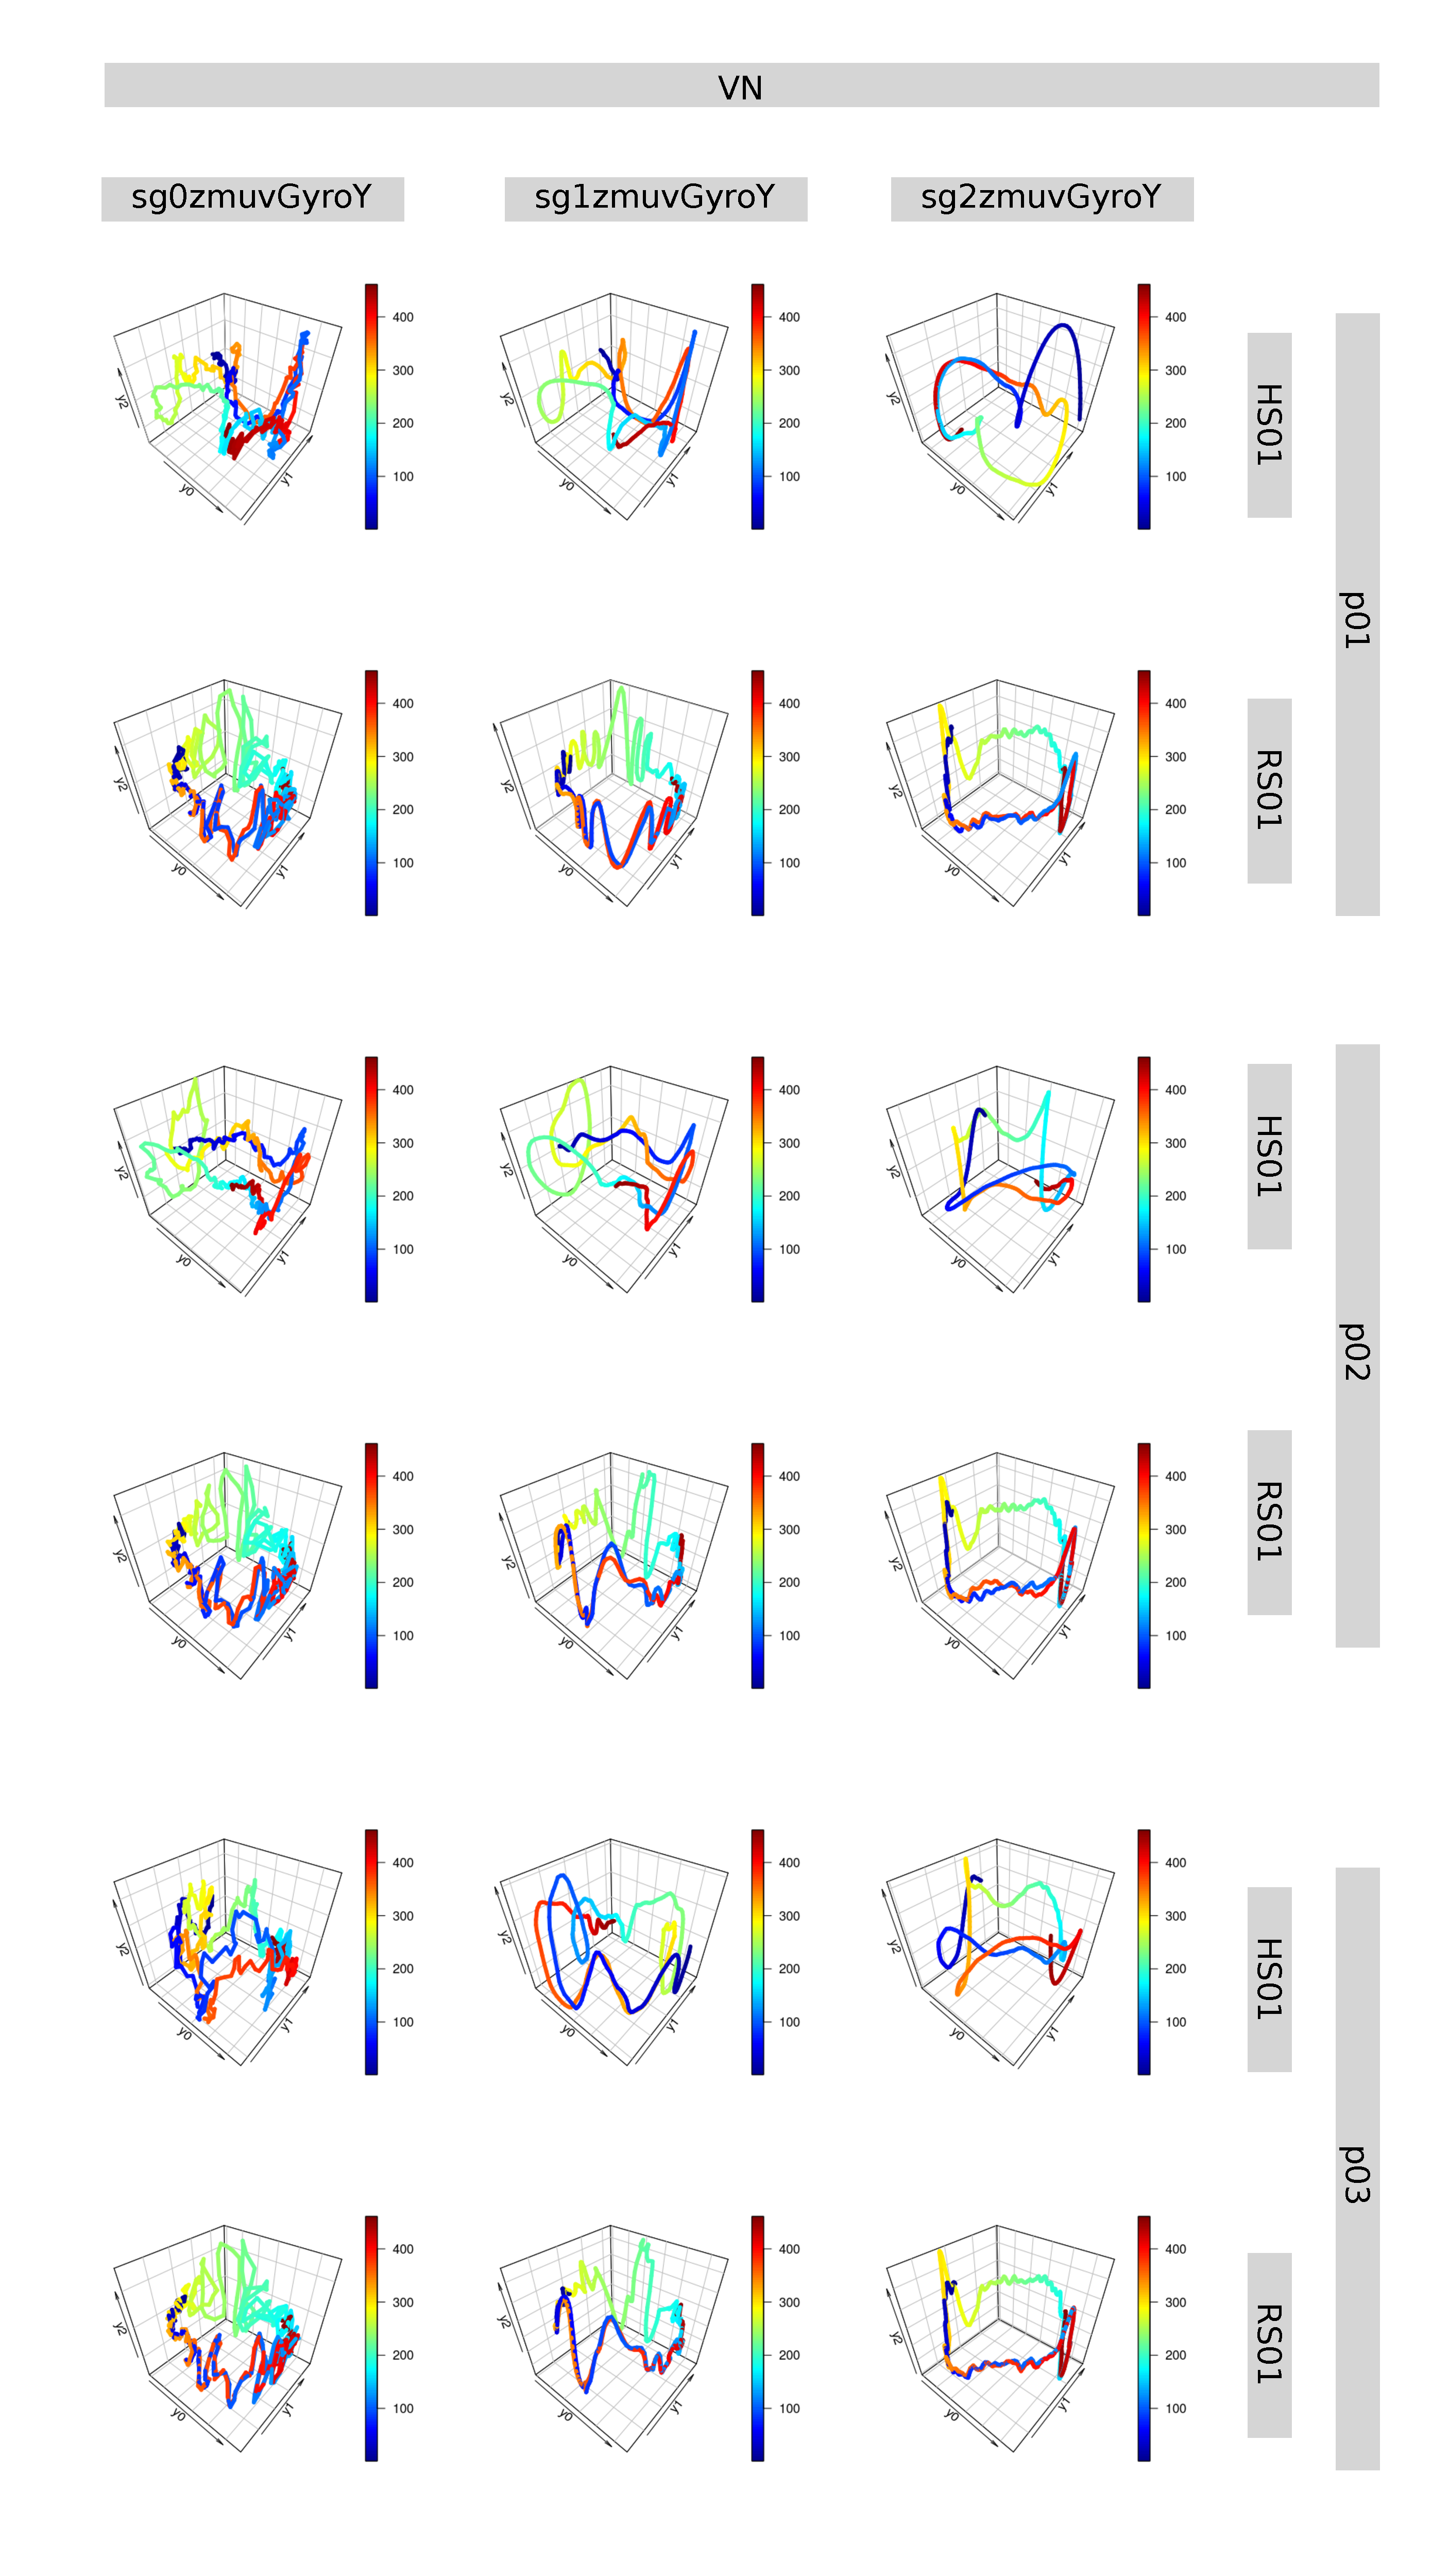
\includegraphics[height=0.85\textheight]{rss_VN}
\caption
	[RSSs for vertical normal arm movements]{
	{\bf RSSs for vertical normal arm movements.}
	Reconstructed state spaces %for time series of Figure \ref{fig:tsH}.
	of participant $p01$, $p02$ and $p03$ for horizontal movements 
	with raw-normalised (sg0zmuvGyroY), 
	normalised-smoothed 1 (sg1zmuvGyroY) and 
	normalised-smoothed 2 (sg2zmuvGyroY) time series of the 
	sensors attached to the participant (HS01) and other sensor 
	attached to the robot (RS01).	
	Reconstructed state spaces were computed with 
	embedding parameters $m=6$, $\tau=8$.
	R code to reproduce the figure is available from \cite{xochicale2018}.
        }
    \label{fig:rss_VN}
\end{figure}
%%---------------------------------(FIGURE)------------------------------------

%%---------------------------------(FIGURE)-------------------------------------
\begin{figure}
\centering
\includegraphics[height=0.85\textheight]{rss_VF}
\caption
	[RSSs for vertical faster arm movements]{
	{\bf RSSs for vertical faster arm movements.}
	Reconstructed state spaces %for time series of Figure \ref{fig:tsH}.
	of participant $p01$, $p02$ and $p03$ for horizontal faster movements 
	with raw-normalised (sg0zmuvGyroY), 
	normalised-smoothed 1 (sg1zmuvGyroY) and 
	normalised-smoothed 2 (sg2zmuvGyroY) time series of the 
	sensors attached to the participant (HS01) and other sensor 
	attached to the robot (RS01).	
	Reconstructed state spaces were computed with 
	embedding parameters $m=6$, $\tau=8$.
	R code to reproduce the figure is available from \cite{xochicale2018}.
        }
    \label{fig:rss_VF}
\end{figure}
%%---------------------------------(FIGURE)------------------------------------







\newpage
\section{RPs} \label{appendix:e:rps}


Recurrence Plots participant $p01$, $p02$ and $p03$ 
for horizontal arm movements (Figs. \ref{fig:rp_HN}, \ref{fig:rp_HF})
and vertical arm movements   (Figs. \ref{fig:rp_VN}, \ref{fig:rp_VF}).
For remained results with window size lengths of time series data, 
we refer the reader to download the data and code at \cite{xochicale2018}.



%%---------------------------------(FIGURE)-------------------------------------
\begin{figure}
\centering
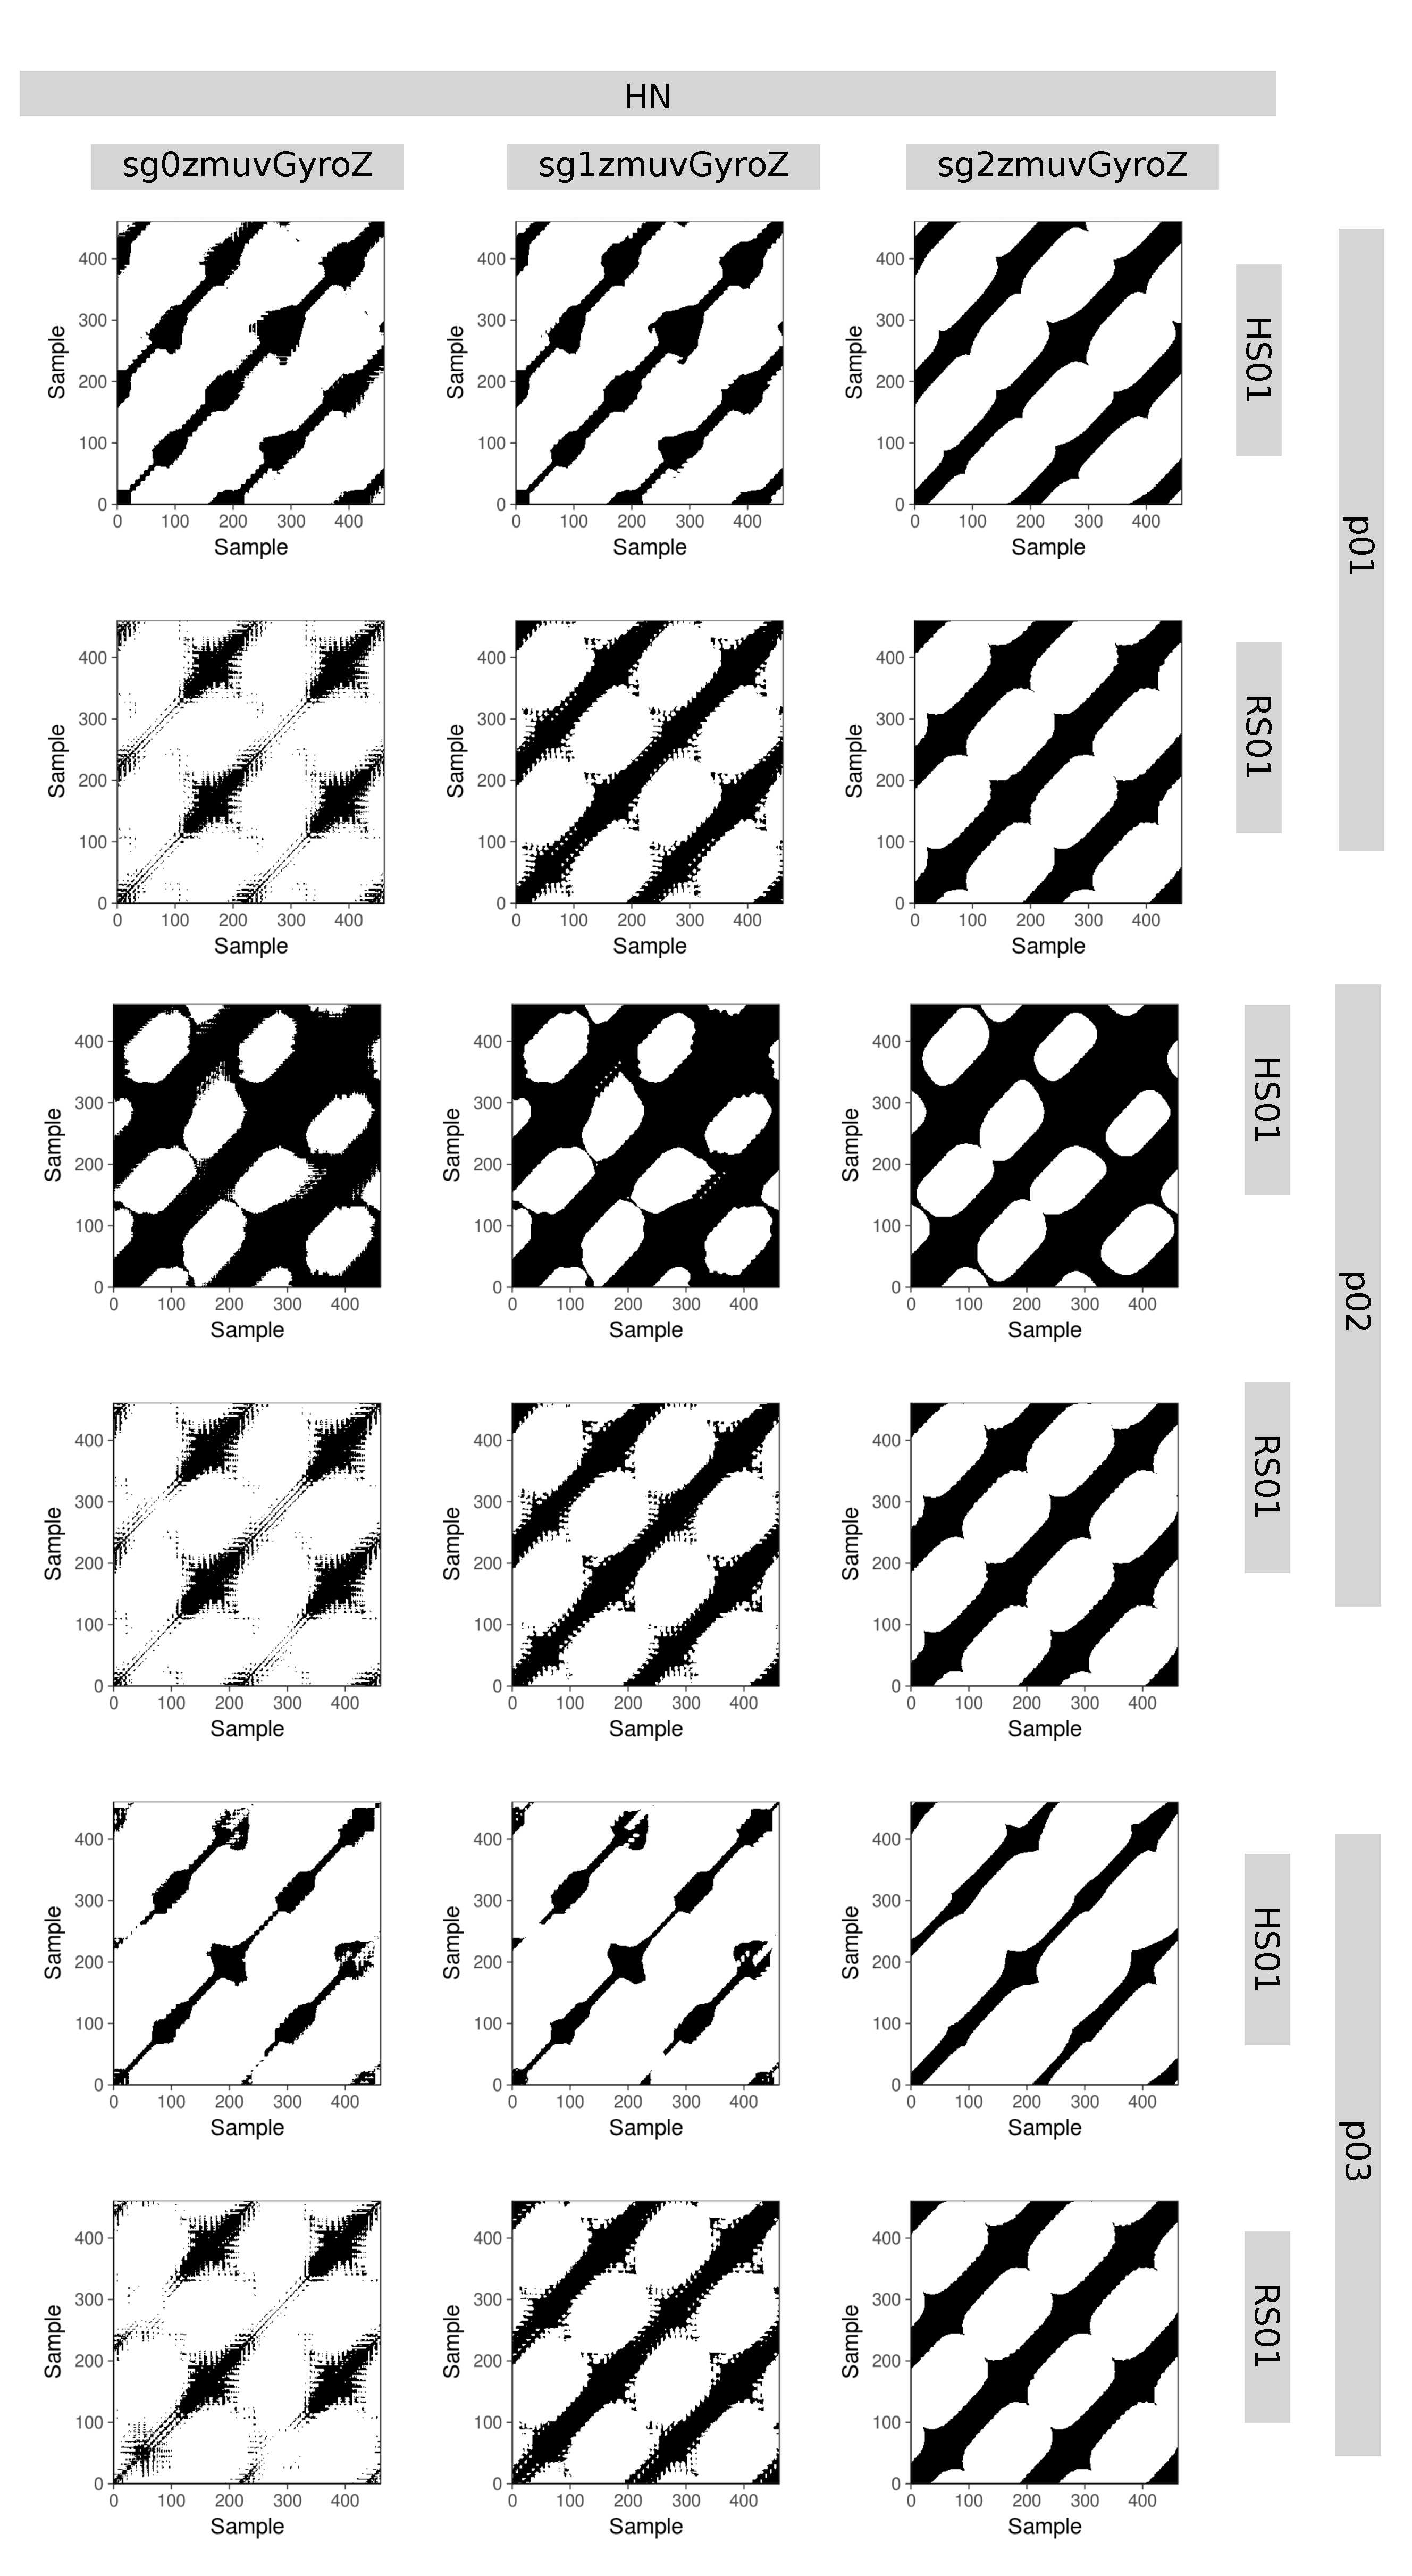
\includegraphics[height=0.80\textheight]{rp_HN}
\caption
	[RPs for horizontal normal arm movements]{
	{\bf RPs for horizontal normal arm movements.}	
	Recurrence plots %for time series of Figure \ref{fig:tsV}.
	of participant $p01$, $p02$, $p03$ for horizontal normal 
	movements with time series of raw-normalised (sg0zmuvGyroZ), 
	normalised-smoothed 1 (sg1zmuvGyroZ) and 
	normalised-smoothed 2 (sg2zmuvGyroZ), and 
	sensors attached to the participant (HS01) and to the robot (RS01).
	Recurrence plots were computed with 
	embedding parameters $m=6$, $\tau=8$ and $\epsilon=1$.
	R code to reproduce the figure is available from \cite{xochicale2018}.
        }
    \label{fig:rp_HN}
\end{figure}
%%---------------------------------(FIGURE)------------------------------------



%%---------------------------------(FIGURE)-------------------------------------
\begin{figure}
\centering
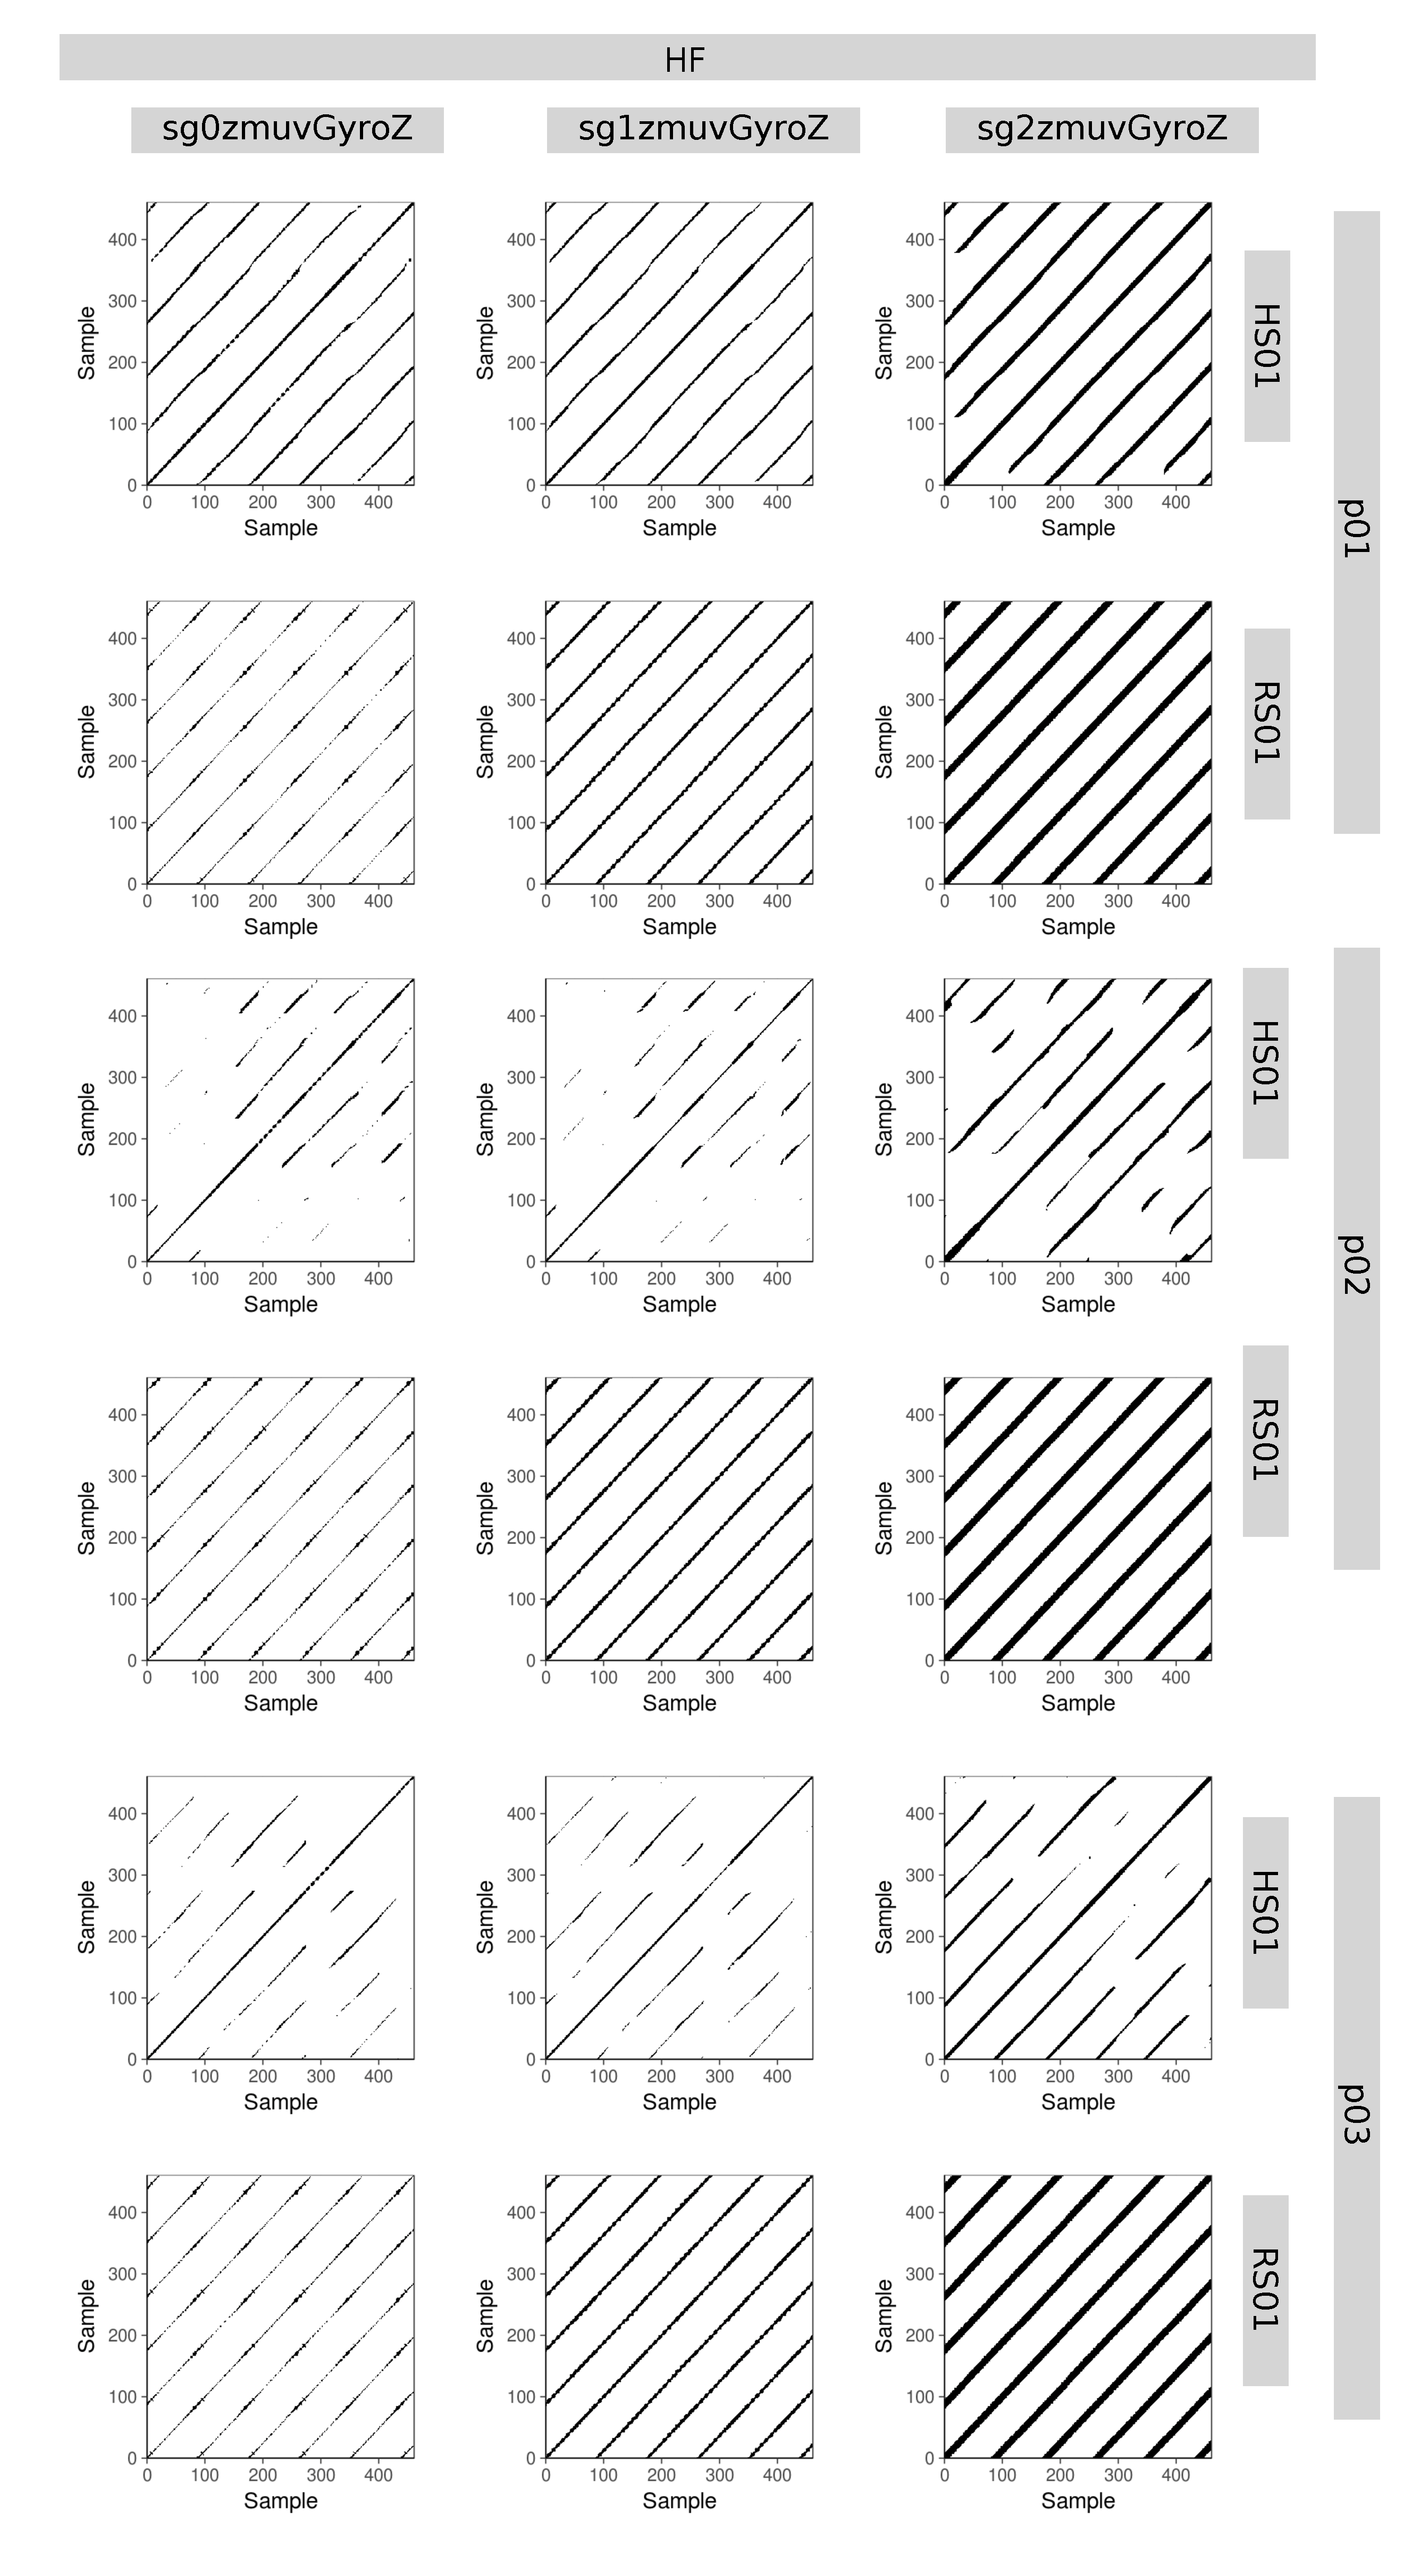
\includegraphics[height=0.80\textheight]{rp_HF}
\caption
	[RPs for horizontal faster arm movements]{
	{\bf RPs for horizontal faster arm movements.}	
	Recurrence plots %for time series of Figure \ref{fig:tsV}.
	of participant $p01$, $p02$, $p03$ for horizontal faster
	movements with time series of raw-normalised (sg0zmuvGyroZ), 
	normalised-smoothed 1 (sg1zmuvGyroZ) and 
	normalised-smoothed 2 (sg2zmuvGyroZ), and 
	sensors attached to the participant (HS01) and to the robot (RS01).
	Recurrence plots were computed with 
	embedding parameters $m=6$, $\tau=8$ and $\epsilon=1$.
	R code to reproduce the figure is available from \cite{xochicale2018}.
        }
    \label{fig:rp_HF}
\end{figure}
%%---------------------------------(FIGURE)------------------------------------







%%---------------------------------(FIGURE)-------------------------------------
\begin{figure}
\centering
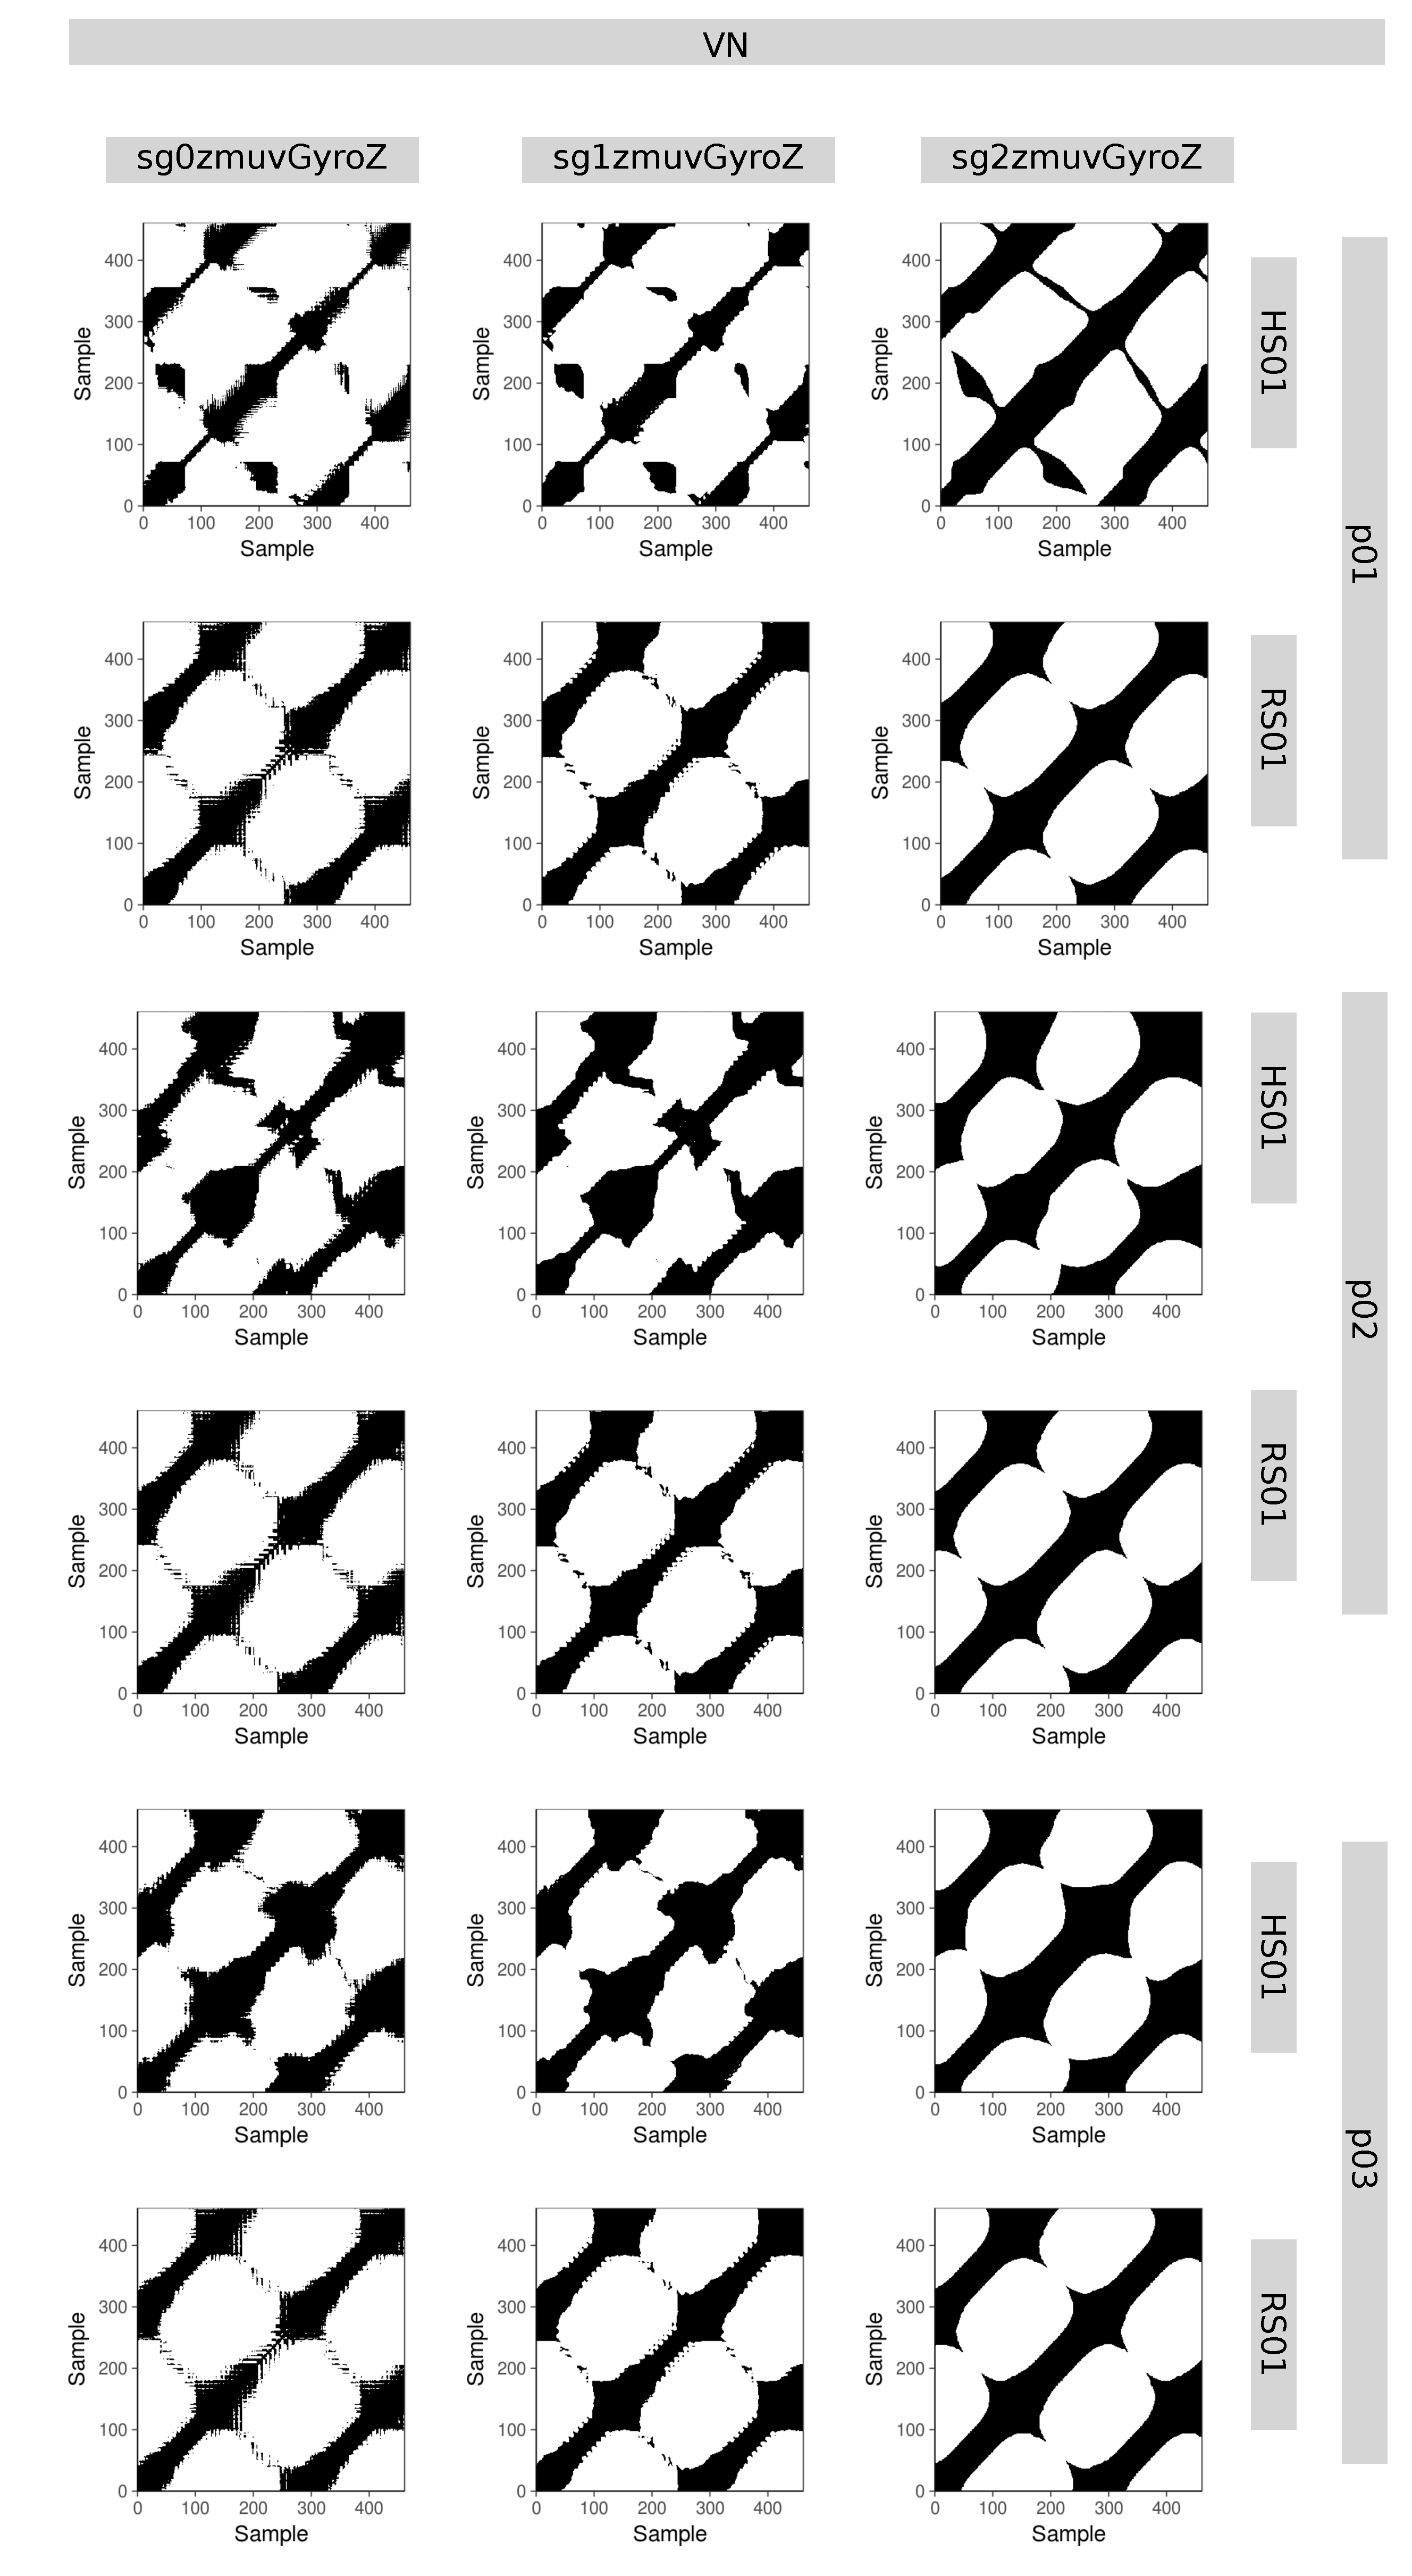
\includegraphics[height=0.80\textheight]{rp_VN}
\caption
	[RPs for vertical normal arm movements]{
	{\bf RPs for vertical normal arm movements.}	
	Recurrence plots %for time series of Figure \ref{fig:tsV}.
	of participant $p01$, $p02$, $p03$ for vertical normal 
	movements with time series of raw-normalised (sg0zmuvGyroY), 
	normalised-smoothed 1 (sg1zmuvGyroY) and 
	normalised-smoothed 2 (sg2zmuvGyroY), and 
	sensors attached to the participant (HS01) and to the robot (RS01).
	Recurrence plots were computed with 
	embedding parameters $m=6$, $\tau=8$ and $\epsilon=1$.
	R code to reproduce the figure is available from \cite{xochicale2018}.
        }
    \label{fig:rp_VN}
\end{figure}
%%---------------------------------(FIGURE)------------------------------------



%%---------------------------------(FIGURE)-------------------------------------
\begin{figure}
\centering
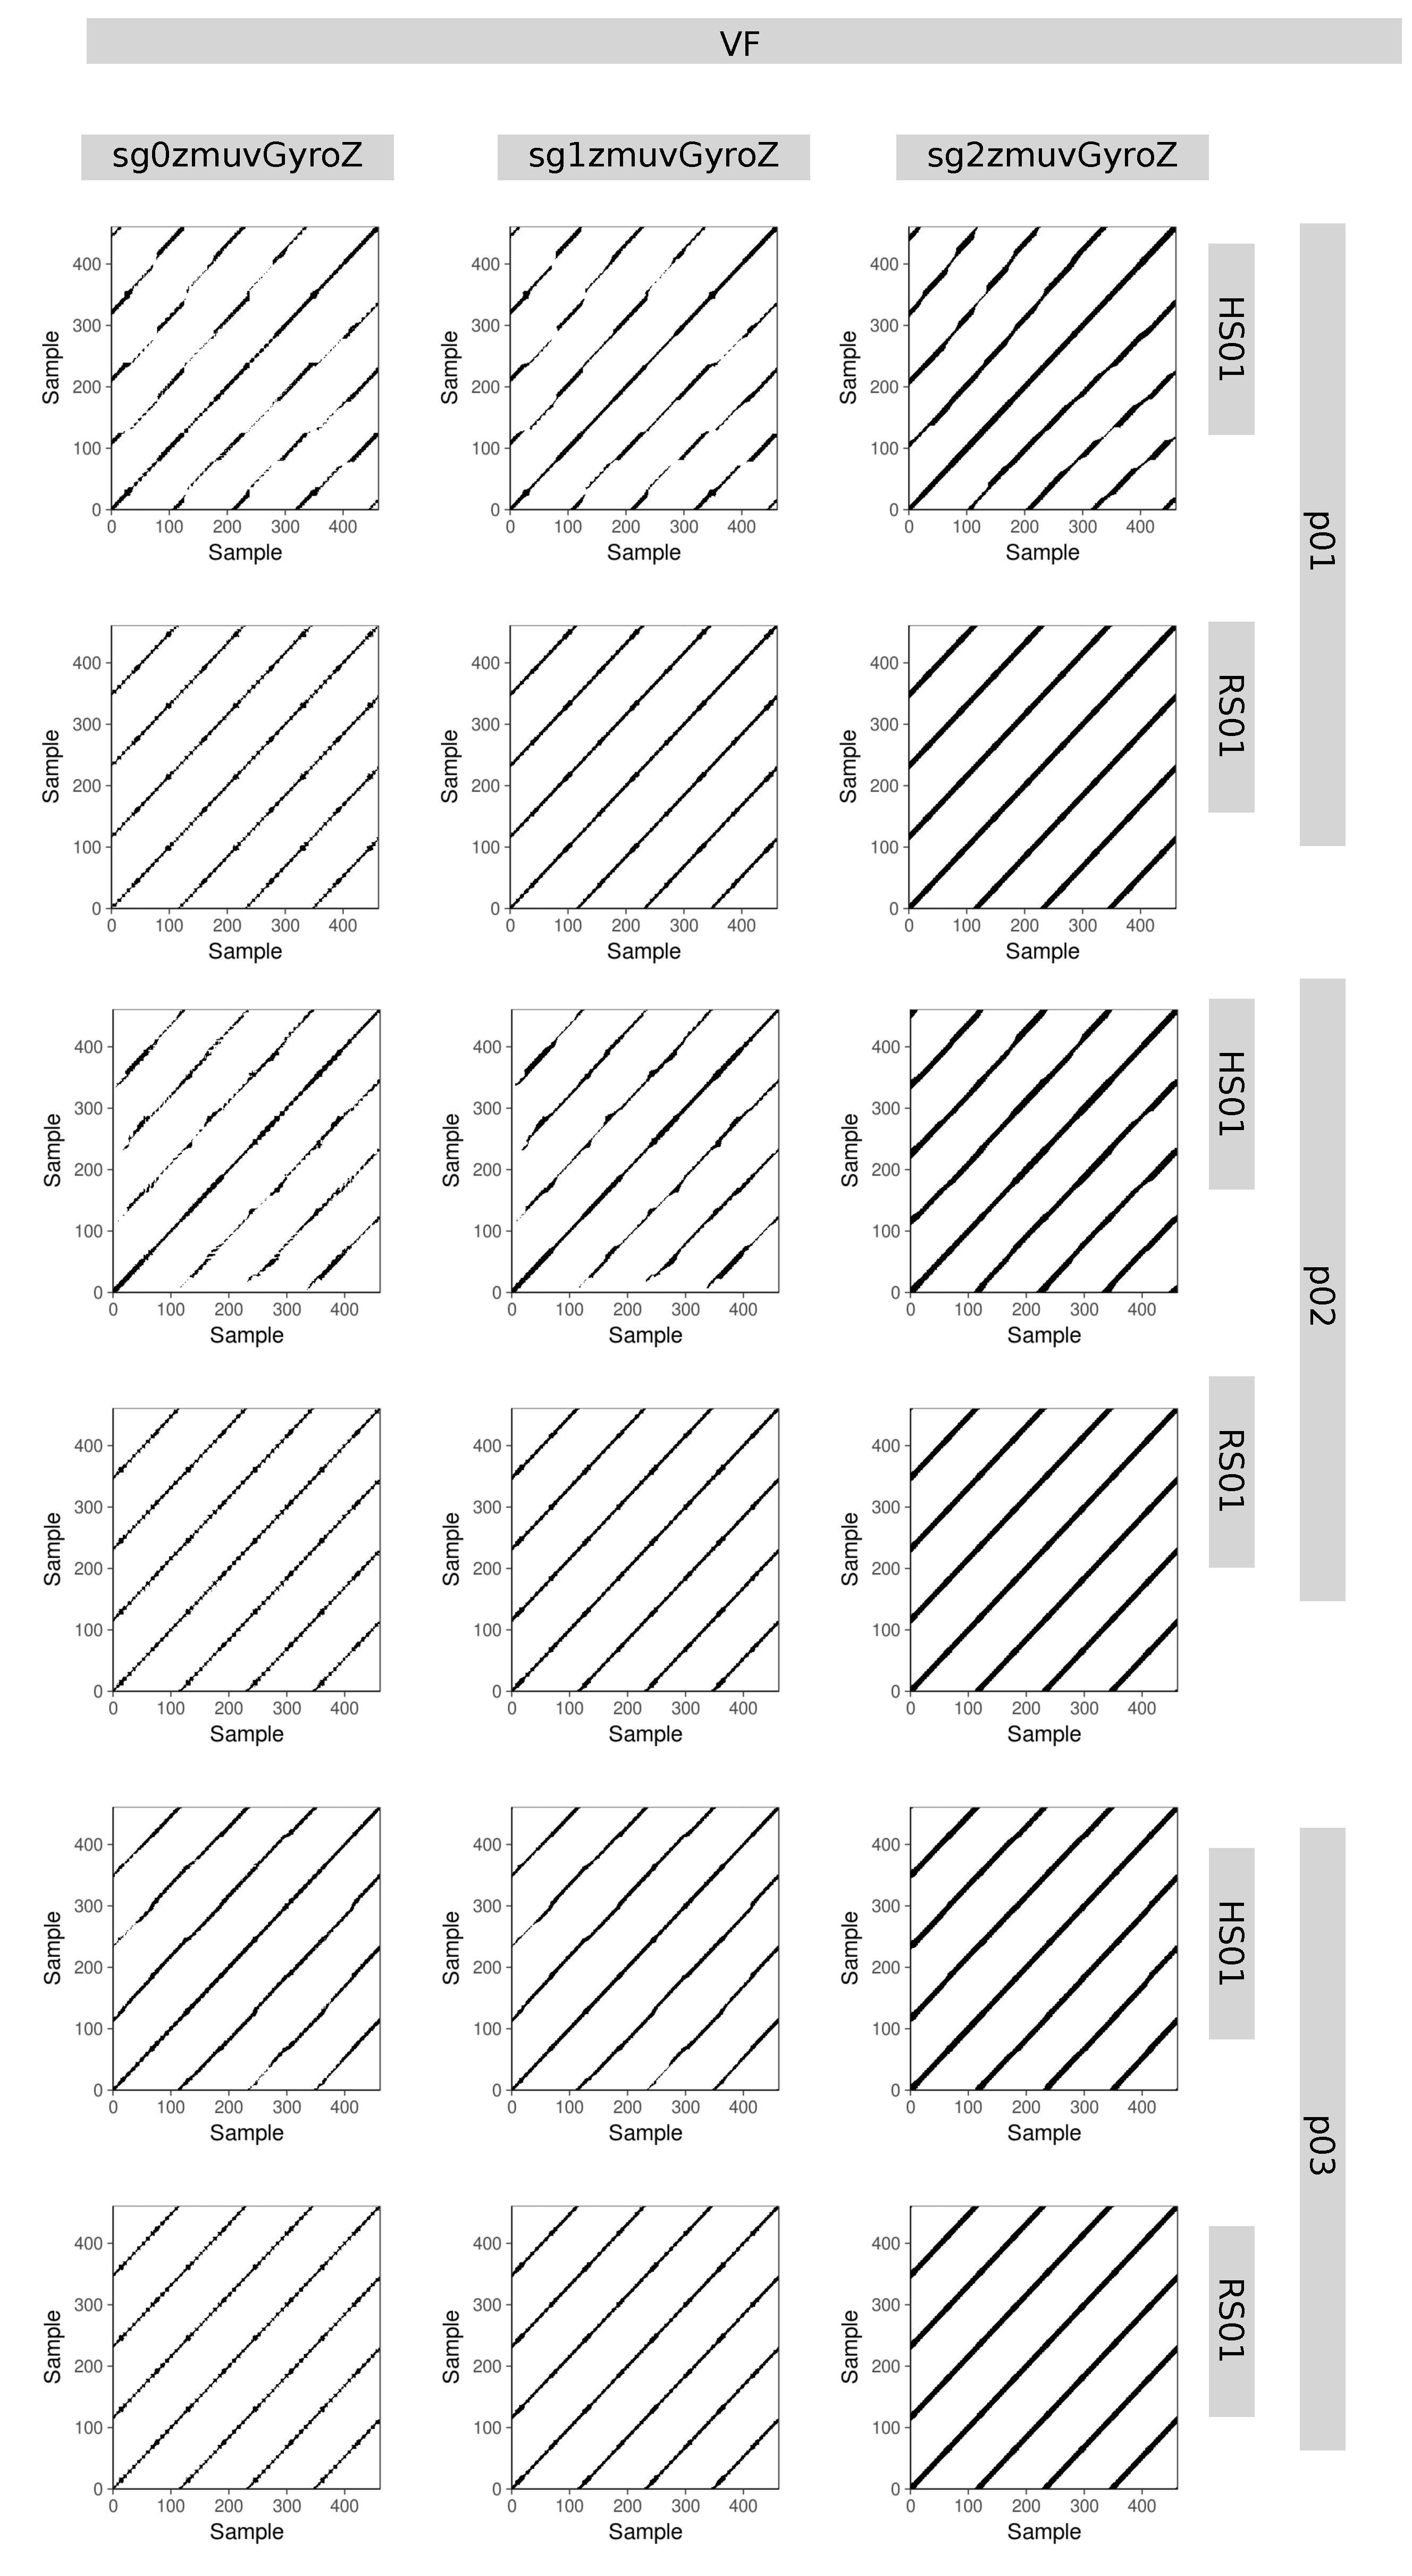
\includegraphics[height=0.80\textheight]{rp_VF}
\caption
	[RPs for vertical faster arm movements]{
	{\bf RPs for vertical faster arm movements.}	
	Recurrence plots %for time series of Figure \ref{fig:tsV}.
	of participant $p01$, $p02$, $p03$ for vertical faster
	movements with time series of raw-normalised (sg0zmuvGyroY), 
	normalised-smoothed 1 (sg1zmuvGyroY) and 
	normalised-smoothed 2 (sg2zmuvGyroY), and 
	sensors attached to the participant (HS01) and to the robot (RS01).
	Recurrence plots were computed with 
	embedding parameters $m=6$, $\tau=8$ and $\epsilon=1$.
	R code to reproduce the figure is available from \cite{xochicale2018}.
        }
    \label{fig:rp_VF}
\end{figure}
%%---------------------------------(FIGURE)------------------------------------




























\newpage
\section{RQAs} \label{appendix:e:rpas}
\subsection{REC values}


REC values, representing the \% of black dots in the RPs, 
are shown in Figs. \ref{fig:rec_aH} and \ref{fig:rec_aV}.



%%---------------------------------(FIGURE)-------------------------------------
\begin{figure}
\centering
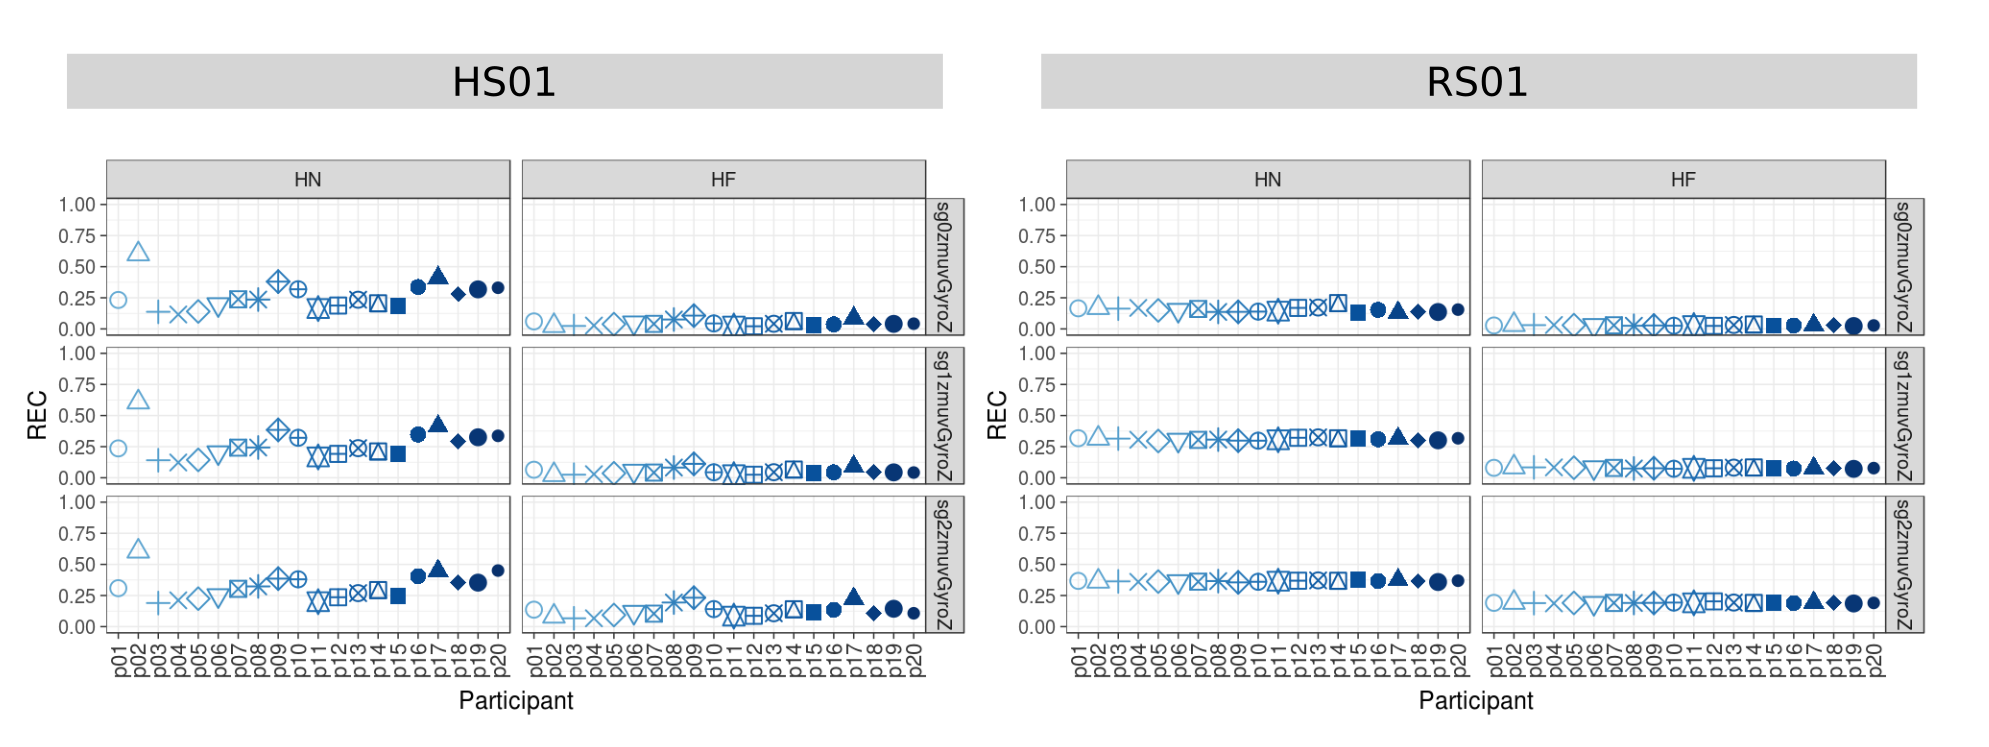
\includegraphics[width=1.0\textwidth]{rec_aH}
    \caption
	[REC values for horizontal arm movements]{
	{\bf REC values for horizontal arm movements.}	
	REC values (representing \% of black dots in the RPs) for 
	20 participants performing HN and HF movements
	with sensors HS01, RS01 and three smoothed-normalised axis 
	of GyroZ (sg0zmuvGyroZ, sg1zmuvGyroZ and sg2zmuvGyroZ).
	REC values were computed with 
	embedding parameters $m=6$, $\tau=8$ and $\epsilon=1$
	R code to reproduce the figure is available from \cite{xochicale2018}.
        }
    \label{fig:rec_aH}
\end{figure}
%%---------------------------------(FIGURE)------------------------------------
%%---------------------------------(FIGURE)-------------------------------------
\begin{figure}
\centering
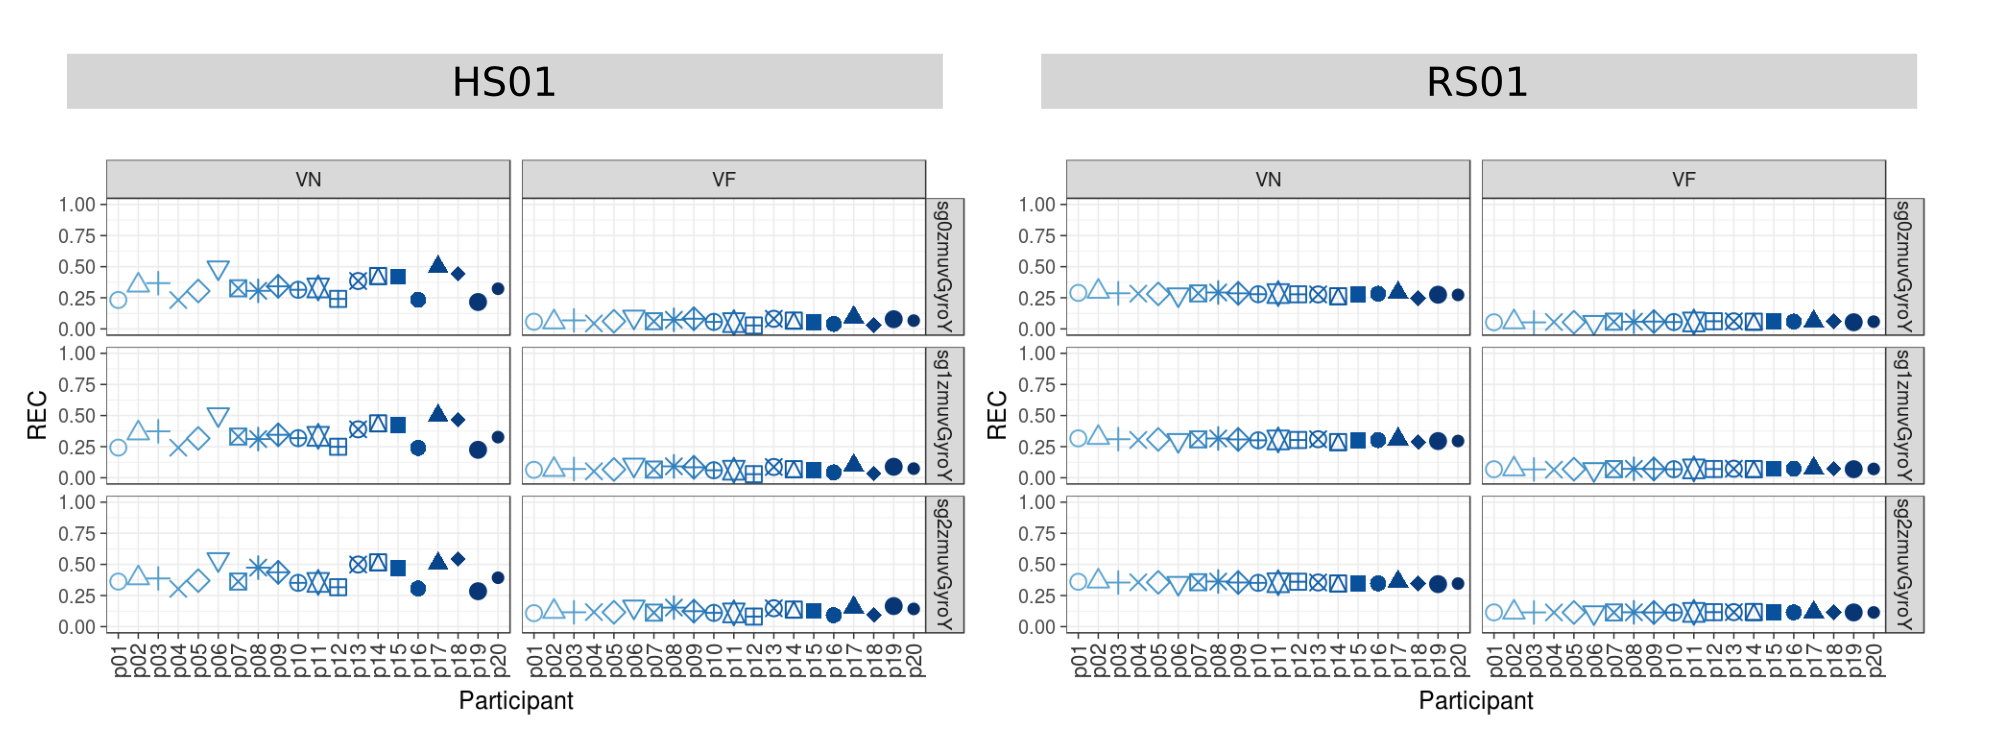
\includegraphics[width=1.0\textwidth]{rec_aV}
    \caption
	[REC values for vertical arm movements]{
	{\bf REC values for vertical arm movements.}	
	REC values (representing \% of black dots in the RPs) for 
	20 participants performing VN and VF movements
	with sensors HS01, RS01 and three smoothed-normalised axis 
	of GyroY (sg0zmuvGyroY, sg1zmuvGyroY and sg2zmuvGyroY).
	REC values were computed with 
	embedding parameters $m=6$, $\tau=8$ and $\epsilon=1$.
	R code to reproduce the figure is available from \cite{xochicale2018}.
        }
    \label{fig:rec_aV}
\end{figure}
%%---------------------------------(FIGURE)------------------------------------


\newpage
\subsection{DET values}
DET values, representing predictability and organisation of the RPs.
are shown in Figs. \ref{fig:det_aH} and \ref{fig:det_aV}.


%%---------------------------------(FIGURE)-------------------------------------
\begin{figure}
\centering
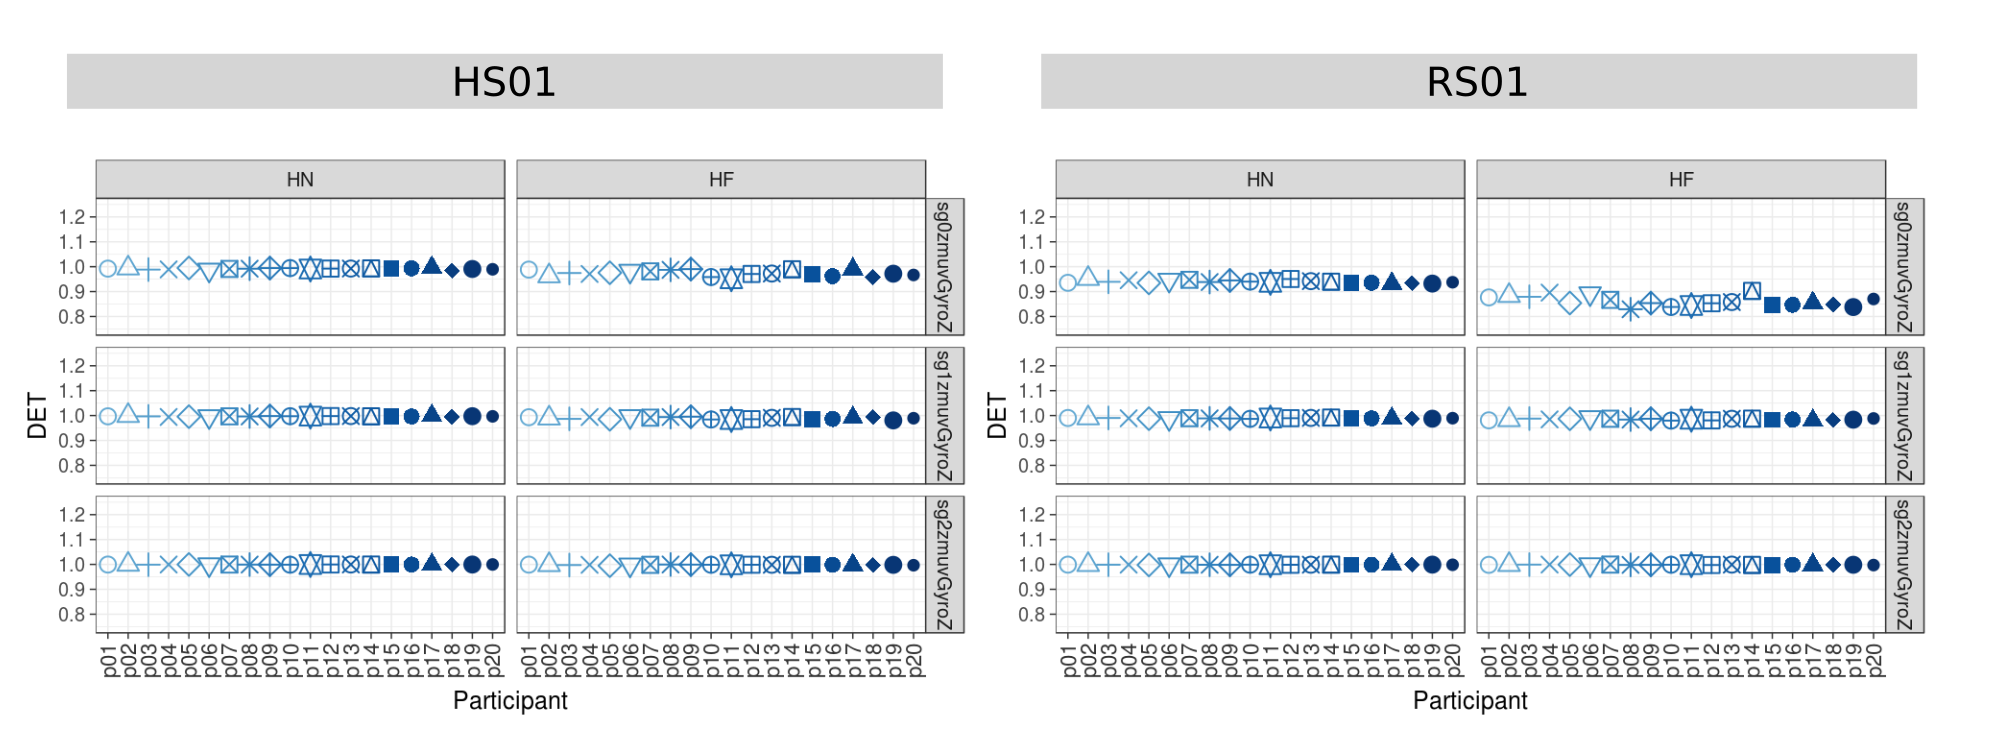
\includegraphics[width=1.0\textwidth]{det_aH}
    \caption
	[DET values for horizontal arm movements]{
	{\bf DET values for horizontal arm movements.}	
    	DET values (representing predictability and organisation of the RPs)
	for 20 participants performing HN and HF movements
	with sensors HS01, RS01 and three smoothed-normalised axis 
	of GyroZ (sg0zmuvGyroZ, sg1zmuvGyroZ and sg2zmuvGyroZ).
	DET values were computed with 
	embedding parameters $m=6$, $\tau=8$ and $\epsilon=1$.
	R code to reproduce the figure is available from \cite{xochicale2018}.
        }
    \label{fig:det_aH}
\end{figure}
%%---------------------------------(FIGURE)------------------------------------
%%---------------------------------(FIGURE)-------------------------------------
\begin{figure}
\centering
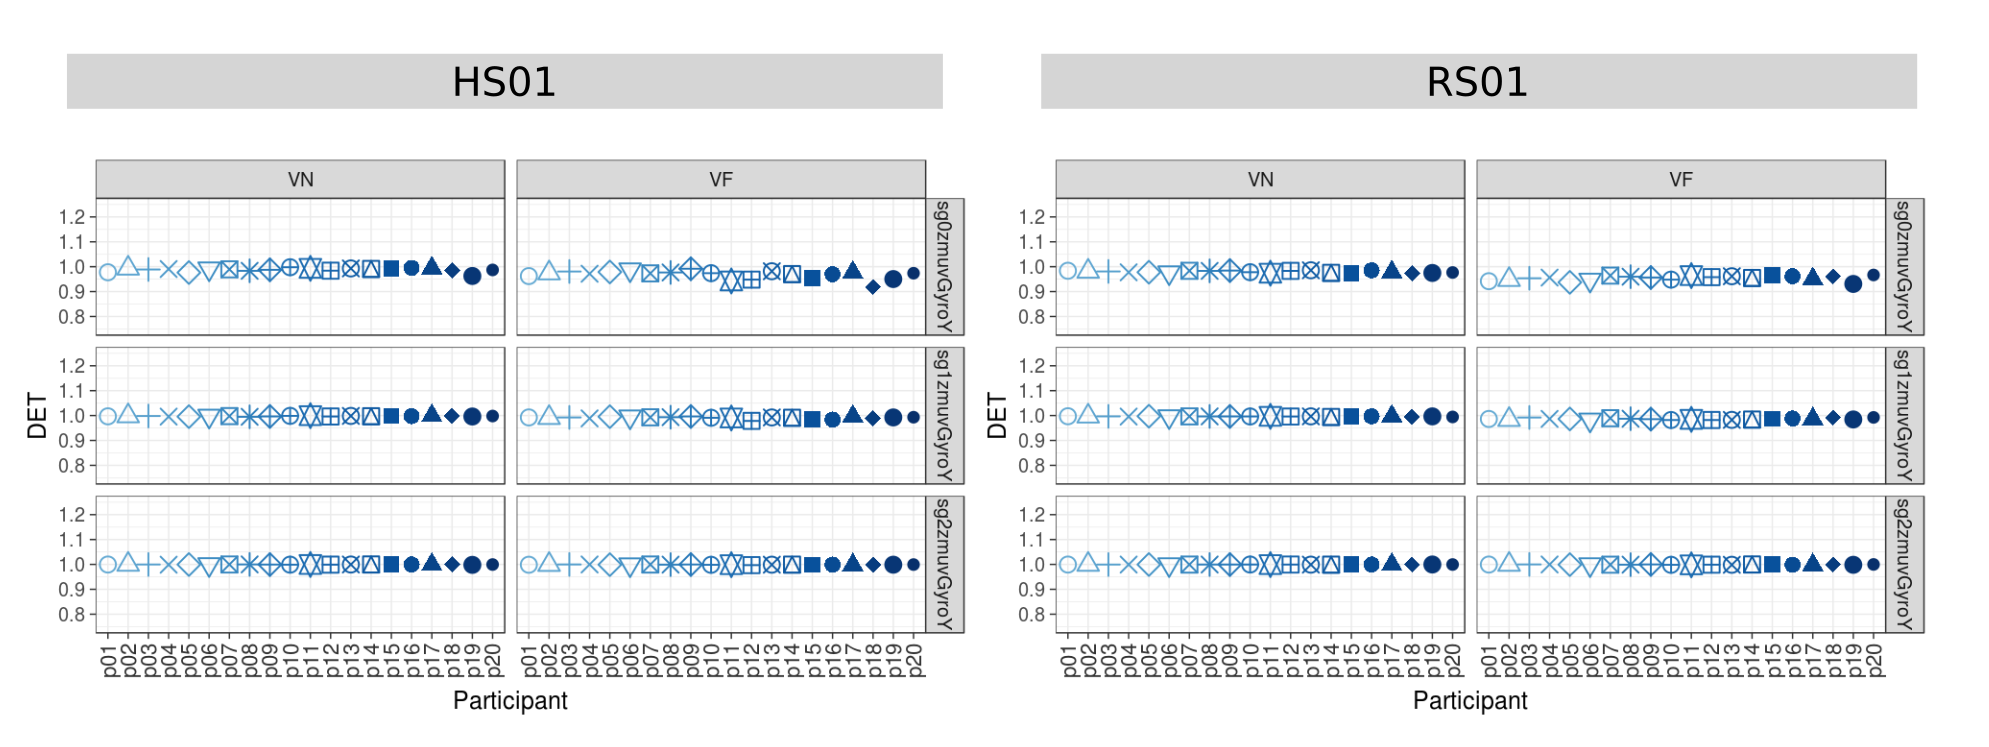
\includegraphics[width=1.0\textwidth]{det_aV}
    \caption
	[DET values for vertical arm movements]{
	{\bf DET values for vertical arm movements.}	
    	DET values (representing predictability and organisation of the RPs) 
	for 20 participants performing VN and VF movements
	with sensors HS01, RS01 and three smoothed-normalised axis 
	of GyroY (sg0zmuvGyroY, sg1zmuvGyroY and sg2zmuvGyroY).
	DET values were computed with 
	embedding parameters $m=6$, $\tau=8$ and $\epsilon=1$.
	R code to reproduce the figure is available from \cite{xochicale2018}.
        }
    \label{fig:det_aV}
\end{figure}
%%---------------------------------(FIGURE)------------------------------------



\newpage
\subsection{RATIO values}
RATIO values, representing dynamic transitions, 
are shown in Figs. \ref{fig:ratio_aH} and \ref{fig:ratio_aV}.


%%---------------------------------(FIGURE)-------------------------------------
\begin{figure}
\centering
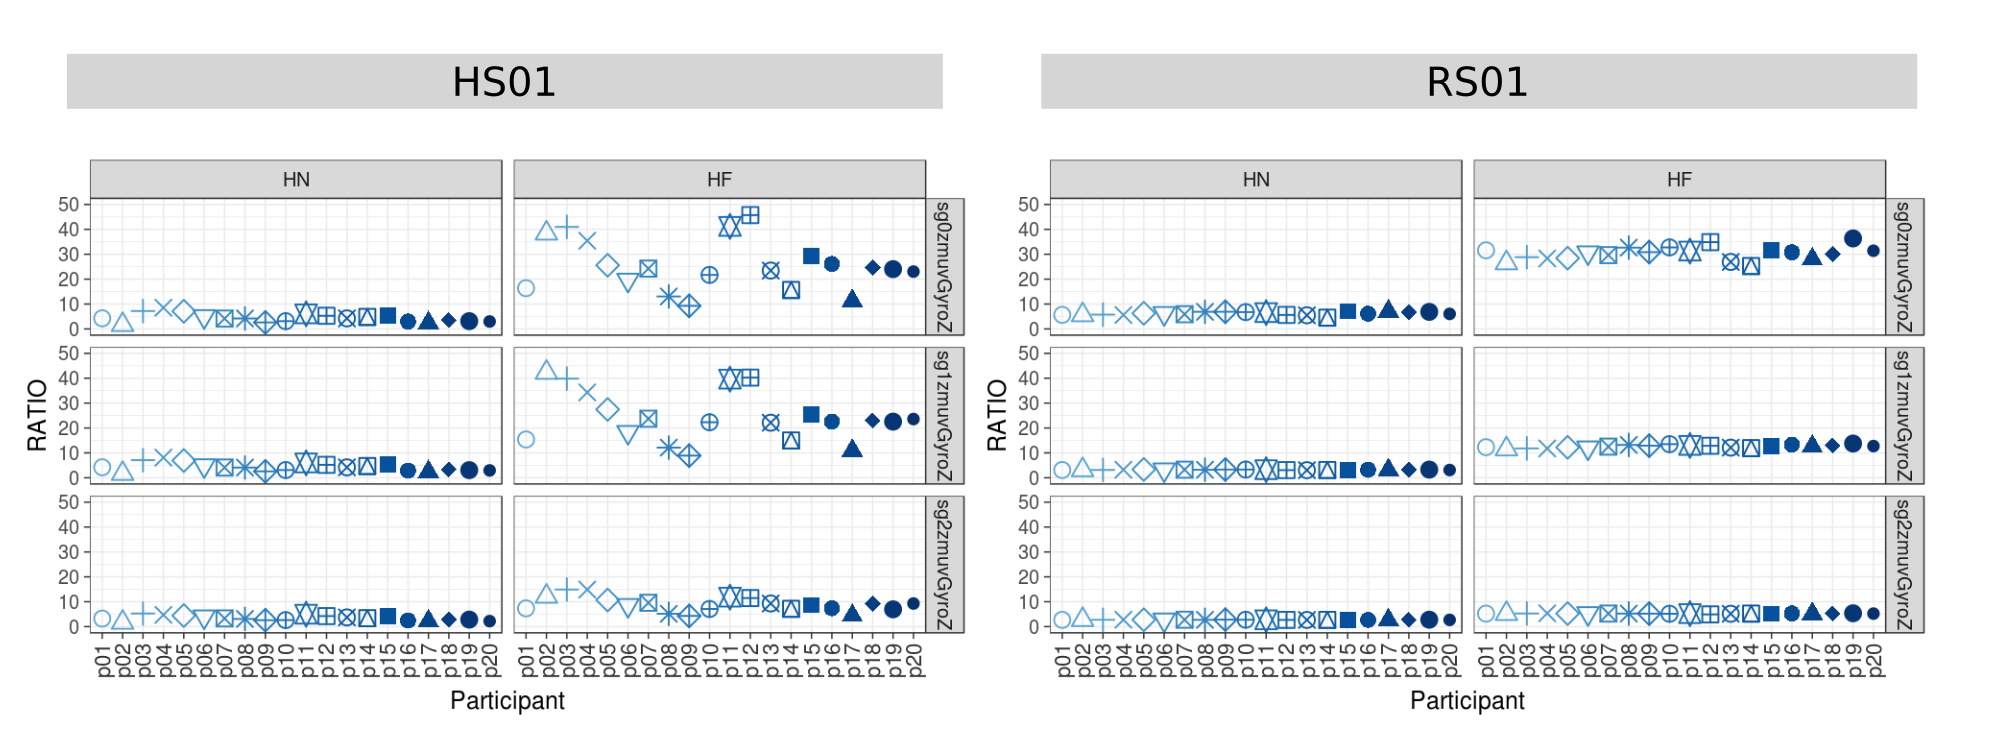
\includegraphics[width=1.0\textwidth]{ratio_aH}
    \caption
	[RATIO values for horizontal arm movements]{
	{\bf RATIO values for horizontal arm movements.}
	RATIO (representing dynamic transitions) for 
	20 participants performing HN and HF movements
	with sensors HS01, RS01 and three smoothed-normalised axis 
	of GyroZ (sg0zmuvGyroZ, sg1zmuvGyroZ and sg2zmuvGyroZ).
	RATIO values were computed with 
	embedding parameters $m=6$, $\tau=8$ and $\epsilon=1$.
	R code to reproduce the figure is available from \cite{xochicale2018}.
        }
    \label{fig:ratio_aH}
\end{figure}
%%---------------------------------(FIGURE)------------------------------------
%%---------------------------------(FIGURE)-------------------------------------
\begin{figure}
\centering
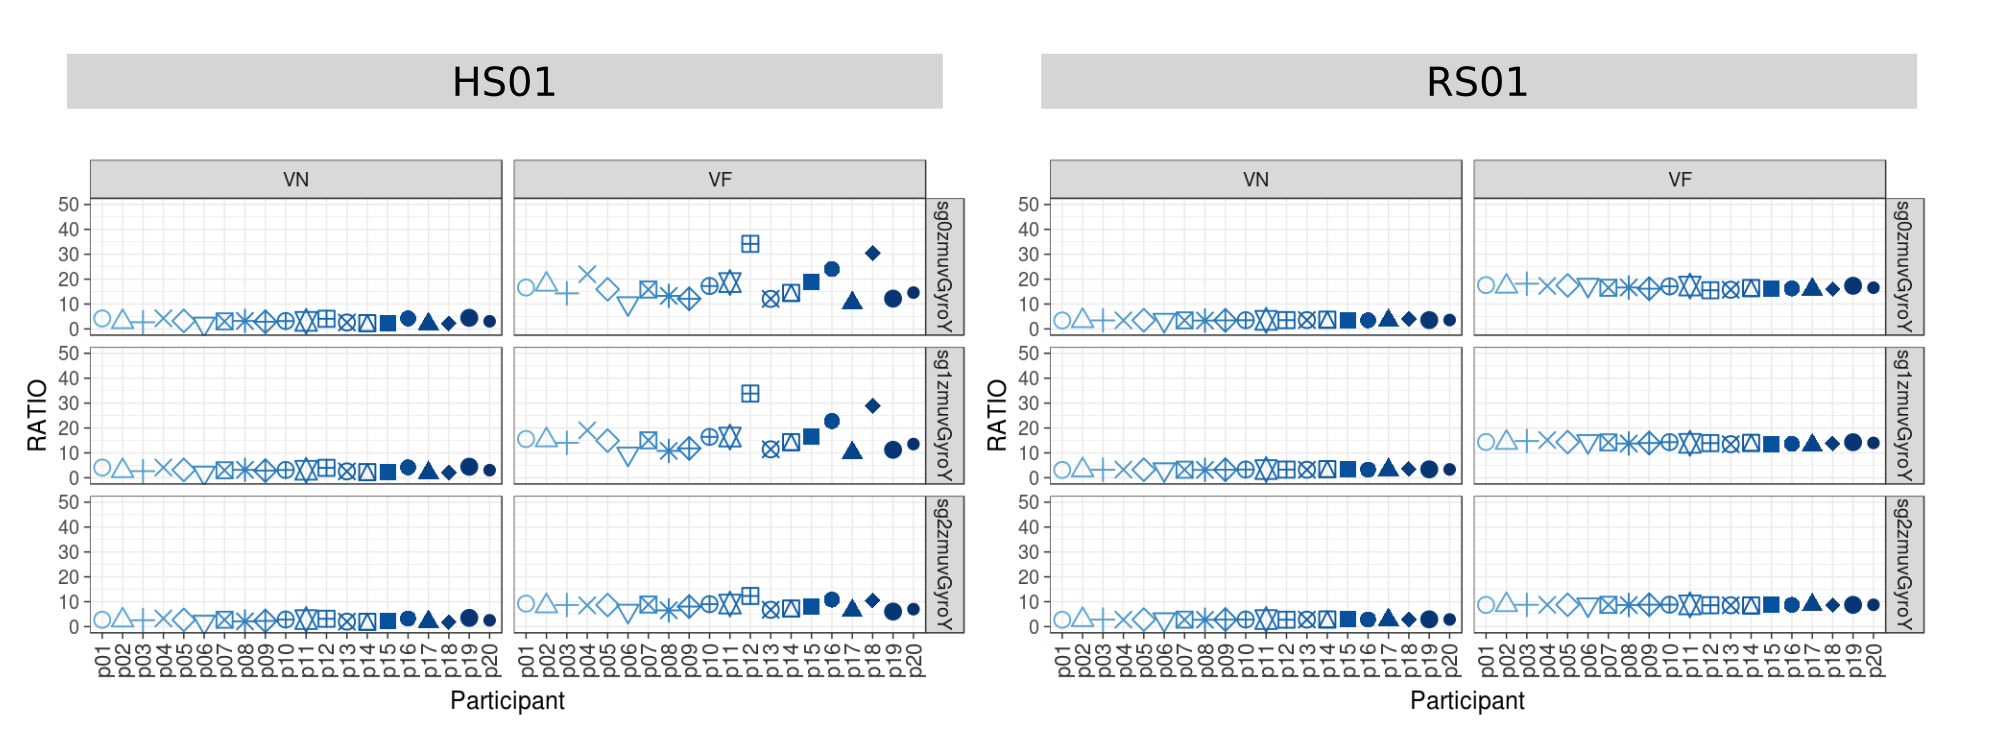
\includegraphics[width=1.0\textwidth]{ratio_aV}
    \caption
	[RATIO values for vertical arm movement]{
	{\bf RATIO values for vertical arm movements.}
	RATIO (representing dynamic transitions) for 
	20 participants performing VN and VF movements
	with sensors HS01, RS01 and three smoothed-normalised axis 
	of GyroY (sg0zmuvGyroY, sg1zmuvGyroY and sg2zmuvGyroY).
	RATIO values were computed with
	embedding parameters $m=6$, $\tau=8$ and $\epsilon=1$.
	R code to reproduce the figure is available from \cite{xochicale2018}.
        }
    \label{fig:ratio_aV}
\end{figure}
%%---------------------------------(FIGURE)------------------------------------



\newpage
\subsection{ENTR values}
ENTR values, representing the complexity of the ructure in time series,
are shown in Figs. \ref{fig:entr_aH} and \ref{fig:entr_aV}.

%%---------------------------------(FIGURE)-------------------------------------
\begin{figure}
\centering
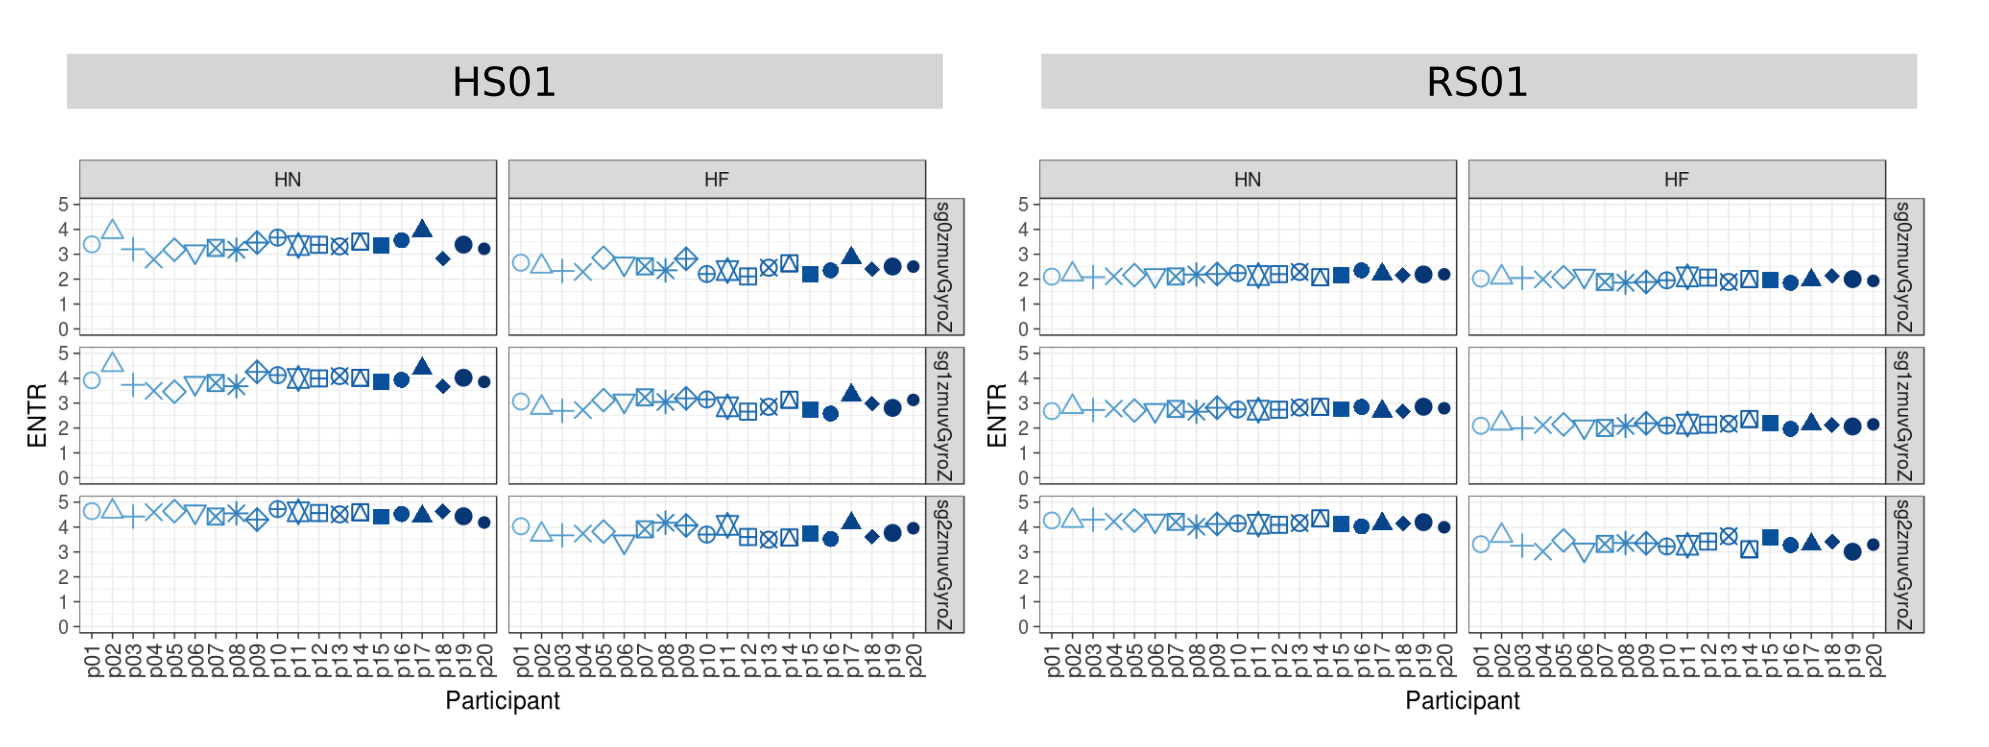
\includegraphics[width=1.0\textwidth]{entr_aH}
    \caption
	[ENTR values for horizontal arm movements]{
	{\bf ENTR values for horizontal arm movements.}
    	ENTR values (representing the complexity of the deterministic 
	structure in time series) for 
	20 participants performing HN and HF movements
	with sensors HS01, RS01 and three smoothed-normalised axis 
	of GyroZ (sg0zmuvGyroZ, sg1zmuvGyroZ and sg2zmuvGyroZ).
	ENTR values were computed with 
	embedding parameters $m=6$, $\tau=8$ and $\epsilon=1$.
	R code to reproduce the figure is available from \cite{xochicale2018}.
        }
    \label{fig:entr_aH}
\end{figure}
%%---------------------------------(FIGURE)------------------------------------
%%---------------------------------(FIGURE)-------------------------------------
\begin{figure}
\centering
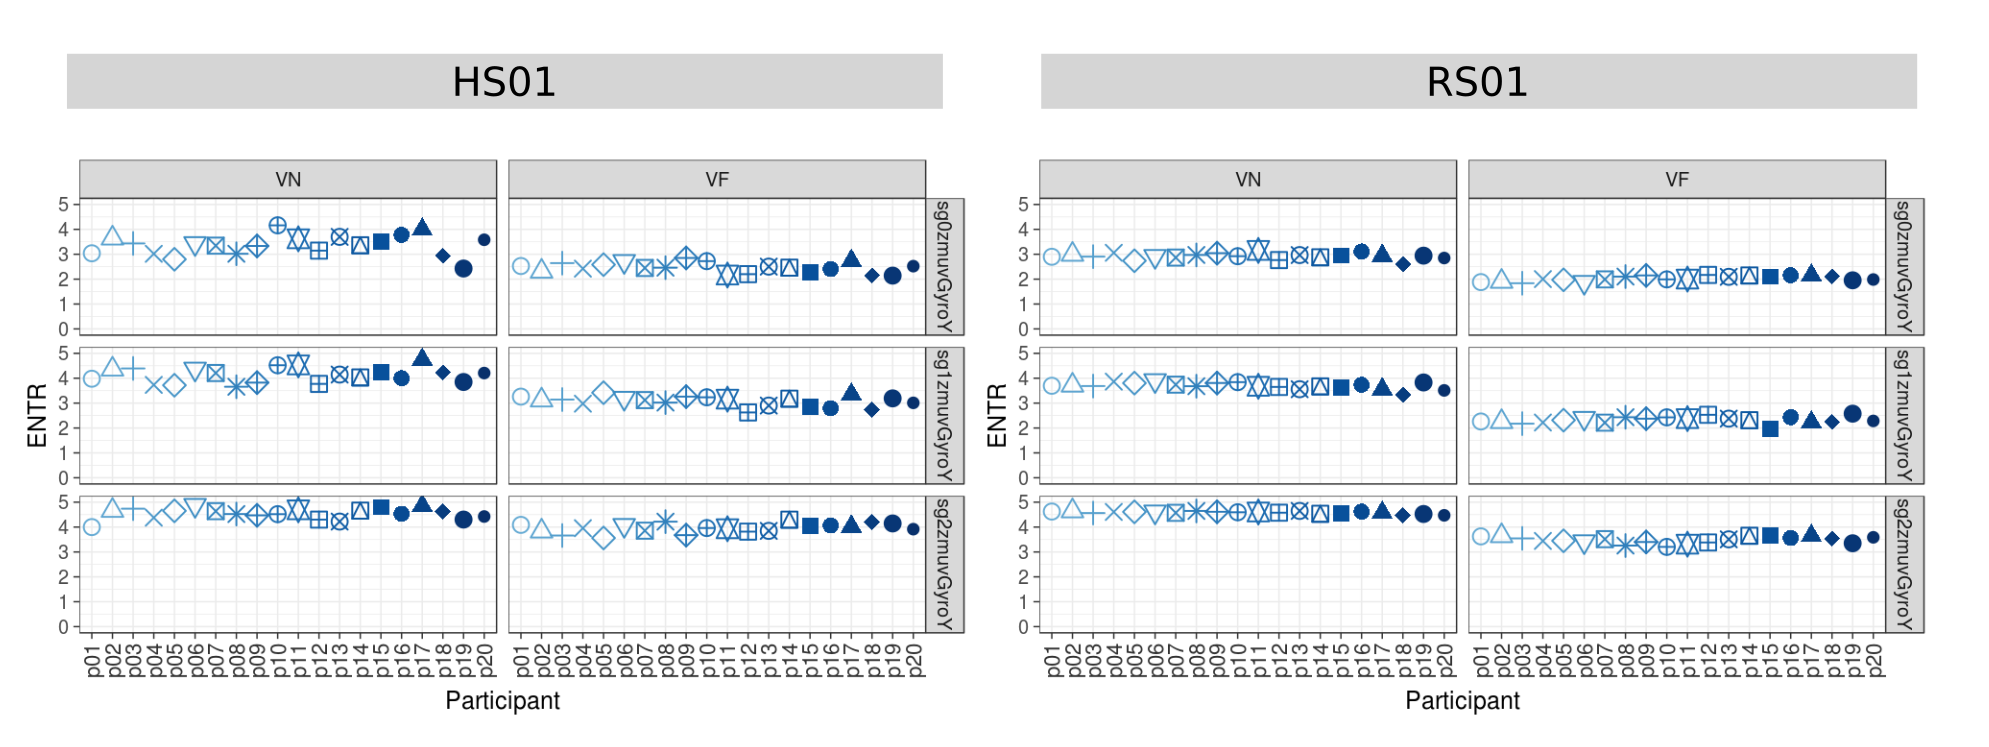
\includegraphics[width=1.0\textwidth]{entr_aV}
    \caption
	[ENTR values for vertical arm movements]{
	{\bf ENTR values for vertical arm movements.}
    	ENTR values (representing the complexity of the deterministic 
	structure in time series) for 
	20 participants performing VN and VF movements
	with sensors HS01, RS01 and three smoothed-normalised axis 
	of GyroY (sg0zmuvGyroY, sg1zmuvGyroY and sg2zmuvGyroY).
	ENTR values were computed with 
	embedding parameters $m=6$, $\tau=8$ and $\epsilon=1$.
	R code to reproduce the figure is available from \cite{xochicale2018}.
        }
    \label{fig:entr_aV}
\end{figure}
%%---------------------------------(FIGURE)------------------------------------





